\documentclass[11pt, a4paper]{article} % , draft
\usepackage[utf8]{inputenc}

\usepackage{enumitem} % customiçe item dots etc
\usepackage{textgreek} % obv
\usepackage{physics} % for easy derivative notation
\usepackage{amsmath}
\usepackage{amsthm} %theorems
\usepackage{amssymb}
\usepackage{mathtools} % for matrices with blocks inside
\usepackage[scr=boondoxo]{mathalfa}
\usepackage{pst-node}%
\usepackage{mathrsfs}
\DeclareMathAlphabet{\mathpzc}{OT1}{pzc}{m}{it}

\newcommand{\mc}{\multicolumn{1}{c}}
\newcommand{\R}{\mathbb{R}} % command for real R
\newcommand{\Holo}{\mathcal{H}}
\newcommand{\M}{\mathcal{M}}
\newcommand{\C}{\mathbb{C}}
\newcommand{\N}{\mathbb{N}}
\newcommand{\z}{\mathpzc{s}}
\newcommand{\p}{\mathpzc{r}}
\newcommand{\s}{\mathbb{S}}
\newcommand{\W}{\mathbb{W}}
\newcommand{\U}{\mathscr{U}}
\usepackage{csquotes}
\MakeOuterQuote{"}
\setlength{\parskip}{0.3 cm}


%\usepackage{nath} % authomatic parenthesis stuff
%\delimgrowth=1
\usepackage[left=2cm, right=2cm, top=2.1cm, bottom=2.1cm]{geometry} % set custom margins
\usepackage{graphicx} % to insert figures
\usepackage{grffile}
\graphicspath{{Figures/}} % define the figure folder path
\usepackage{subcaption} % for multiple figures at once each with a caption
\usepackage{multirow} %multirow in tables

\usepackage{caption}
\captionsetup[figure]{font=footnotesize} %adjust caption size
\captionsetup[table]{font=footnotesize} %adjust caption size

\usepackage{booktabs} % for pretty tabs in tables
\usepackage{siunitx} % Required for alignment
\captionsetup{labelfont=bf} % bold face captations

\usepackage{hyperref} % makes every reference a hyperlink
\hypersetup{
    colorlinks=true,
    linkcolor=violet,
    filecolor=[rgb]{0.69, 0.19, 0.38},      
    urlcolor=[rgb]{0.0, 0.81, 0.82},
    citecolor=[rgb]{0.69, 0.19, 0.38}
}

\usepackage{epigraph} % for quotations in teh begginig
\setlength\epigraphwidth{8cm}
\setlength\epigraphrule{0pt}
\usepackage{etoolbox}
\makeatletter
\patchcmd{\epigraph}{\@epitext{#1}}{\itshape\@epitext{#1}}{}{}
\renewcommand{\qedsymbol}{o.\textepsilon.\textdelta}

\newtheorem{prop}{Proposition} %so I can use propositions
\newtheorem{cor}{Corollary} %so I can use corollaries
\newtheorem{defi}{Definition} %so I can use corollaries

\makeatother % all this is for the epigraph
\usepackage{imakeidx} % make index
\makeindex[columns=3, title=Alphabetical Index, intoc]

\title{\vspace{-2.0cm} {\bf Towards an Improvement of the \\ Hermitian Approximation:\\ \vspace{+0.3cm}{\small Evolving Conditional Wave-Functions\\ without the Full Wave-Function} \vspace{-0.5cm}} \vspace{0.2cm} \\ }
\date{\vspace{-11ex}}
\let\clipbox\relax
\usepackage{adjustbox}
\newcolumntype{?}{!{\vrule width 1.5pt}}
\usepackage{abstract}
\setlength{\absleftindent}{0mm}
\setlength{\absrightindent}{0mm}

\usepackage{listings}
\usepackage{xcolor}
\lstset{language=C++,
                basicstyle=\ttfamily,
                keywordstyle=\color{blue}\ttfamily,
                stringstyle=\color{red}\ttfamily,
                commentstyle=\color{green}\ttfamily,
                morecomment=[l][\color{magenta}]{\#}
    backgroundcolor=\color{black!5}, % set backgroundcolor
    basicstyle=\footnotesize,% basic font setting
}

\begin{document}
\maketitle
\tableofcontents
\pagenumbering{gobble}
\clearpage
\pagenumbering{arabic}
\setcounter{page}{1}
\vspace{-0.3 cm}
\section{The Exact Schrödinger-like Equation for Conditional Wave-Functions}

Given a closed quantum system with $N$ degrees of freedom described by the spatial variables $\vec{x}=(x_1,...,x_N)\in \R^n$, the sate of which is given by the normalized full $N$ dimensional wavefunction $\Psi(\vec{x},t)$, its dynamics are governed by the time dependent Schrödinger Equation (TDSE):
\begin{equation}\label{TDSE}\tag{TDSE}
i\hbar \pdv{\Psi(\vec{x}, t)}{t} = - \sum_{k=1}^{N} \frac{\hbar^2}{2m_k}\pdv[2]{\Psi(\vec{x},t)}{x_k} + U(\vec{x},t)\Psi(\vec{x},t)
\end{equation}
where $U(\vec{x},t)$ is the time dependant potential energy field that bends the wavefunction, $\{m_k\}_{k=0}^N$ are the masses of each degree of freedom, $\hbar$ is the experimentally fixed Planck constant and $i=\sqrt{-1}$. The unitary time evolution of the TDSE will allow $\forall t$: $ \int_{-\infty}^\infty \Psi(\vec{x},t)^\dagger \Psi(\vec{x},t) d\vec{x}=1 $, if it is so for $t=t_0$.

We can evolve a trajectory for the quantum system, given an initial point $\vec{x}(t_0)\in \R^N$, by interpreting the spatial variation of the phase of the full wavefunction as its velocity field (following Bohmian Mechanics). That is, defining the velocity field for the $k$-th dimension as:
$$
v_k(\vec{x},t) = \frac{\hbar}{m_k}\pdv{ Phase(\Psi(\vec{x},t))}{x_k}=\frac{\hbar}{m_k}\mathbb{I}m\qty(\Psi^{-1}(\vec{x},t)\pdv{}{x_k}\Psi(\vec{x},t))
$$
Then, given the point $\vec{x}(t_0)\in \R^N$, the trajectory $\vec{x}(t)$ crossing it at $t_0$ will be uniquely defined by:
$$
\dv{}{t}x^\beta_k(t)=v_k(\vec{x}(t),t) \quad \forall k\in \{1,...,N\}\vspace{-0.05 cm}
$$
Given a particular Bohmian Trajectory for the system, that we will label with $\beta$, $\vec{x}^\beta(t)$, we will define for each $x_a\in\{x_k\}_{k=1}^N$ the degrees of freedom of the rest of the system as $\vec{x_b}=(x_1,...,x_{a-1},x_{a+1},...,x_N)$. Now, let us define the Conditional Wavefunction (CWF) for $x_a$, given the $\beta$-th Bohmian trajectory for the rest of degrees of freedom $\vec{x}_b^\beta(t)$, as:
\begin{equation}\label{CWF}\tag{CWF}
\psi_a^\beta(x_a,t) := \Psi(x_a, \vec{x}_b^\beta(t), t)\vspace{-0.05 cm}
\end{equation}
Note that the ordinary differential equations ruling the trajectory can be solved even if we only knew the CWF-s! This is because each $a$-th velocity field is obtained by a derivative of the same spatial variable. As such, they only depend on the CWF-s:
$$
\dv{}{t}x^\beta_a(t)=v_a(x_a^\beta (t), \vec{x}^\beta_b(t),t)=\frac{\hbar}{m_k}\mathbb{I}m\qty(\psi_a^\beta(x_a, t)^{-1}\pdv{}{x_k}\psi_a^\beta(x_a, t),t) \quad \forall a\in \{1,...,N\}
$$
In what follows we will show three different ways to exactly arrive to a set of Schrödinger like equations for the conditional wave-functions. We will call them in general "the exact Schrödinger like Equations for Conditional Wave-Functions" and shorten them by \label{CWF.SE}\hyperlink{CWF.SE}{(CWF.SE)}. \vspace{-0.3 cm}

\subsection{Shape I for \hyperref[CWF.SE]{CWF.SE}: The Kinetic and Advective Correlation Potentials}

Given the Bohmian Trajectory for the system labelled by $\beta$, $\vec{x}^\beta(t)$, for each $x_a\in\{x_k\}_{k=1}^N$ we can condition the full wavefunction in the TDSE to the trajectory for $\vec{x}_b=(x_1,...,x_{a-1},x_{a+1},...,x_N)$:
$$
i\hbar \pdv{\Psi(\vec{x}, t)}{t}\Big\rvert_{\vec{x}_b=\vec{x}(t)_b^\beta} = - \sum_{k=1}^{N} \frac{\hbar^2}{2m_k}\pdv[2]{\Psi(\vec{x},t)}{x_k}\Big\rvert_{\vec{x}_b=\vec{x}_b^\beta(t)} + U(\vec{x},t)\Big\rvert_{\vec{x}_b=\vec{x}(t)_b^\beta}\Psi(\vec{x},t)\Big\rvert_{\vec{x}_b=\vec{x}(t)_b^\beta}
$$
Noting that by the chain rule:
$$
\dv{\Psi(x_a, \vec{x}_b^\beta(t), t)}{t} = \pdv{\Psi(\vec{x}, t)}{t}\Big\rvert_{\vec{x}_b=\vec{x}(t)_b^\beta} + \sum_{\substack{k=1; \\ k\neq a}}^{N} \pdv{\Psi(\vec{x}, t)}{x_k}\Big\rvert_{\vec{x}_b=\vec{x}(t)_b^\beta} \dot{x}_k^\beta(t)
$$
We get:\vspace{-0.3cm}
$$
i\hbar \dv{\Psi(x_a, \vec{x}_b^\beta(t), t)}{t} = - \frac{\hbar^2}{2m_a}\pdv[2]{\Psi(x_a, \vec{x}_b^\beta(t), t)}{x_a} + U(x_a, \vec{x}_b^\beta(t), t)\Psi(x_a, \vec{x}_b^\beta(t), t) 
$$
$$
- \sum_{\substack{k=1; \\ k\neq a}}^{N} \frac{\hbar^2}{2m_k}\pdv[2]{\Psi(\vec{x},t)}{x_k}\Big\rvert_{\vec{x}_b=\vec{x}_b^\beta(t)} + i \hbar  \sum_{\substack{k=1; \\ k\neq a}}^{N} \pdv{\Psi(\vec{x}, t)}{x_k}\Big\rvert_{\vec{x}_b=\vec{x}(t)_b^\beta} \dot{x}_k^\beta(t)\vspace{-0.2cm}
$$

Where we see that all the terms introducing an explicit dependence from the rest of the system ($\vec{x}_b$) on $x_a$, are gathered in the last two terms. Let us define them as the Kinetic Correlation Potential (\ref{K}) and the Advective Correlation Potential (\ref{A}):\vspace{-0.2cm}
\begin{equation}\label{K}\tag{K}
K(x_a, \vec{x}_b^\beta(t), t) = - \ \sum_{\substack{k=1; \\ k\neq a}}^{N} \frac{\hbar^2}{2m_k}\pdv[2]{\Psi(\vec{x},t)}{x_k}\Big\rvert_{\vec{x}_b=\vec{x}_b^\beta(t)}
\end{equation}
\begin{equation}\label{A}\tag{A}
A(x_a, \vec{x}_b^\beta(t), t) =  i \hbar  \sum_{\substack{k=1; \\ k\neq a}}^{N} \pdv{\Psi(\vec{x}, t)}{x_k}\Big\rvert_{\vec{x}_b=\vec{x}(t)_b^\beta} \dot{x}_k^\beta(t)
\end{equation}
They are both complex valued potentials that introduce the correlations (exchange and entanglement) with the rest of the degrees of freedom in the equation (even if $U(x_a, \vec{x}_b^\beta(t), t)$ also introduces some of them). In their terms, the full TDSE can be rewritten as:
\begin{equation*}\label{CWF.SE.I}\tag{CWF.SE.I}
i\hbar \pdv{\psi_a^\beta(x_a, t)}{t} = \qty[- \frac{\hbar^2}{2m_a}\pdv[2]{}{x_a} + U(x_a, \vec{x}_b^\beta(t), t)]\psi_a^\beta(x_a t) + K(x_a, \vec{x}_b^\beta(t), t) +A(x_a, \vec{x}_b^\beta(t), t) \quad
\end{equation*}

We will call this the shape I for the exact conditional wave-function Schrödinger like Equations (\ref{CWF.SE.I}). If we could solve this for each $x_a\in\{x_k\}_{k=1}^N$ given the potential energy $U$, an initial shape for the full wavefunction $\Psi(\vec{x}, t_0)$ and an initial position of the trajectory $\vec{x}^\beta(t_0)$, then we would be evolving the exact shape of the \ref{CWF}-s. For this it would be necessary to evolve the trajectory $\vec{x}^\beta(t)$ in a coupled fashion, which can be obtained from the CWF-s as stated in the introduction.\vspace{-0.2cm}

\subsection{Shape II for \hyperref[CWF.SE]{CWF.SE}:\\ Introducing the Born-Huang ansatz onto the \ref{K},\ref{A} potentials\vspace{-0.2cm}}

As the potential energy $U(\vec{x},t)$ is a known function, for each $x_a\in\{x_k\}_{k=1}^N$  we can define the Transversal Section Eigenstates \ref{TSEig} as the set of functions $\{\Phi_{x_a}^j(\vec{x}_b,t)\}_{j=0}^\infty$ such that:\vspace{-0.2cm}
\begin{equation}\label{TSEig}\tag{TSEig}
\qty(- \sum_{k=1; k\neq a}^{N} \frac{\hbar^2}{2m_k}\pdv[2]{}{x_k}+U(x_a,\vec{x}_b,t) )\Phi_{x_a}^j(\vec{x}_b,t) = E_{x_a}^j(t)\Phi_{x_a}^j(\vec{x}_b,t)
\end{equation}
for $j\in\{0,1,2,3,...\}$. We order the indices $j$ such that the eigenvalues known as energies of the transversal sections fulfill: $E_{x_a}^0(t)\leq E_{x_a}^1(t)\leq E_{x_a}^2(t)...$.

Note that each $\Phi_{x_a}^j(\vec{x}_b,t)$ is a different eigenstate as a function of $a$ (the variable left aside), of where in the domain of $x_a$ we look at and the time in which we look at ($U(x_a,\vec{x}_b,t)$ will vary in $x_a$ and $t$). Thus, we compute these eigenstates for each $a$, $x_a$ and $t$.

As the \ref{TSEig} are the eigenstates of a Hermitian Operator, they can be chosen to satisfy the orthonormality condition on each transversal section Hilbert space. That is:
$$
\int_{-\infty}^\infty \Phi_{x_a}^k(\vec{x}_b,t)^\dagger \Phi_{x_a}^j(\vec{x}_b,t) d\vec{x}_b=\delta_{kj} \equiv \begin{cases}1\ if\ k=j\\0\ if\ k\neq j \end{cases}\quad \forall t\geq t_0
$$
\vspace{-0.2cm}
If the potential $U$ is known, there are plenty of numerical algorithms capable of computing them.

Now, for each $x_a\in\{x_k\}_{k=1}^N$, as the set of (\ref{TSEig}) $\{\Phi_{x_a}^j(\vec{x}_b,t)\}_{j=0}^\infty$ are the eigenstaes of a Hermitian operator, they will be a complete basis for the transversal section Hilbert spaces, meaning we can expand the full wavefunction in their terms as:
\begin{equation}\label{BH}\tag{BH}
\Psi(\vec{x},t)=\sum_{j=0}^\infty \chi_a^j(x_a,t) \Phi_{x_a}^j(\vec{x}_b,t)
\end{equation}
where:
\begin{equation}\label{chi}\tag{chi}
\chi_a^j(x_a,t):= \int_{-\infty}^\infty \Phi_{x_a}^j(\vec{x}_b,t)^\dagger \Psi(\vec{x},t) d\vec{x}_b
\end{equation}
This is the so called Born-Huang expansion (\ref{BH}) of the full wave-function, while the coefficients of the expansion $\{\chi_a^j(x_a,t)\}_{j=0}^\infty$ are called the Adiabatic Coefficients (\ref{chi}).

In particular, if we condition the (\ref{BH}) ansatz to the trajectory $\vec{x}_b^\beta(t)$, we can get an expansion of the \ref{CWF}:
$$
\psi_a^\beta(x_a,t) = \Psi(x_a, \vec{x}_b^\beta(t), t) = \sum_{j=0}^\infty \chi_a^j(x_a,t) \Phi_{x_a}^j(\vec{x}_b^\beta(t),t)
$$

We could now re-write the Kinetic and Advective Correlation potentials (\ref{K}, \ref{A}) in terms of this ansatz:
\begin{equation}\label{K.BH}\tag{K.BH}
K(x_a, \vec{x}_b^\beta(t), t) = -  \sum_{\substack{k=1; \\ k\neq a}}^{N} \sum_{j=0}^\infty \chi_a^j(x_a,t) \frac{\hbar^2}{2m_k} \pdv[2]{ \Phi_{x_a}^j(\vec{x}_b^\beta(t),t)}{x_k}\Big\rvert_{\vec{x}_b=\vec{x}_b^\beta(t)}
\end{equation}
\begin{equation}\label{A.BH}\tag{A.BH}
A(x_a, \vec{x}_b^\beta(t), t) =  i \hbar \sum_{\substack{k=1; \\ k\neq a}}^{N} \sum_{j=0}^\infty \chi_a^j(x_a,t) \pdv{ \Phi_{x_a}^j(\vec{x}_b^\beta(t),t))}{x_k}\Big\rvert_{\vec{x}_b=\vec{x}(t)_b^\beta} \dot{x}_k^\beta(t)
\end{equation}
where we note that unlike the full wave function $\Psi(x_a, \vec{x}_b,t)$, the (\ref{TSEig}) $\Phi_{x_a}^j(\vec{x}_b,t)$ are known, which means their numerical or analytic derivatives will also be known. Thus, we have effectively isolated the unknown out of any derivative in the shape of the coefficients $\chi^j_a(x_a,t)$. The point is that these coefficients still depend on the full wave-function, so we will still be unable to obtain simple expressions for the \ref{CWF}-s. Still, the exact Schrödinger like Equation for the CWF-s (\ref{CWF.SE.I}) can be rewritten in an alternative shape in terms of this Born-Huang ansatz by using (\ref{A.BH}) and (\ref{K.BH}):
\begin{equation}\label{CWF.SE.II}\tag{CWF.SE.II}
i\hbar \pdv{\psi_a^\beta(x_a, t)}{t} = \qty[- \frac{\hbar^2}{2m_a}\pdv[2]{}{x_a} + U(x_a, \vec{x}_b^\beta(t), t)]\psi_a^\beta(x_a t) + K_{BH}(x_a, \vec{x}_b^\beta(t), t) +A_{BH}(x_a, \vec{x}_b^\beta(t), t) 
\end{equation}
where by $ K_{BH}$ and $ A_{BH}$ we mean \ref{K} and \ref{A} but in their Born-Huang ansatz dependence shape given in (\ref{K.BH}) and (\ref{A.BH}).

The fact that the \ref{TSEig} are an orthonormal set makes the norm of the expanded wavefunction to be equal to:
$$
\sum_{j=0}^\infty \int_{-\infty}^\infty \chi_a^j(x_a,t)^\dagger \chi_a^j(x_a,t) dx_a = \int_{-\infty}^\infty \Psi(\vec{x},t)^\dagger \Psi(\vec{x},t)d\vec{x}
$$
the proof is immediate by definition. It could also be seen as a consequence of $\sum_{j=0}^\infty|\chi^j_a(x_a,t)|^2$ being equal to the marginalized probability density $\int_{-\infty}^\infty |\Psi(\vec{x},t)|d\vec{x}_b$, meaning $|\chi^j_a(x_a,t)|^2$ may be interpreted as the density of particles in the transversal section $x_a$ that are in the $k$-th eigenenergy state at time $t$ . Thus, the quantity defined by $\lambda:=\sum_{j=0}^\infty \int_{-\infty}^\infty \qty|\chi_a^j(x_a,t)|^2 dx_a$ can be used as an indicator of which $j$ is big enough as for having captured the biggest part of the sum. That is, if we truncate the sum at $j=J$ such that $\lambda\simeq 1$, then the approximation to the full expansion will be good enough. We call each integral $P_j(t):=\int_{-\infty}^\infty \qty|\chi_a^j(x_a,t)|^2 dx_a$ the Population of the $j-th$ adiabatic level.
\newpage
\subsection{Shape III for \hyperref[CWF.SE]{CWF.SE}: \\ Rewriting \ref{K} and \ref{A} in terms of the CWF - The Real Potentials \ref{G} and \ref{J}}
% Hemen G eta J definidu biher dire
Following the development in Chp.1 V 6 of \cite{JordiXO}: We can try to find a {\bf linear} Schrödinger like equation for the CWF-s employing the following "trick". An arbitrary non-zero single valued complex function $f(x, t):\R^2 \rightarrow \C$ can be imposed to be the solution of a 1D Schrödinger equation:\vspace{-0.3cm}
$$
i \hbar \pdv{f(x,t)}{t} = -\frac{\hbar^2}{2 m}\pdv[2]{f(x,t)}{x} + W(x,t) f(x,t)
$$
if the potential term $W(x, t)$ is defined as:\vspace{-0.3cm}
$$
W(x, t) := \qty(i \hbar \pdv{f(x,t)}{t} +\frac{\hbar^2}{2 m}\pdv[2]{f(x,t)}{x} ) \frac{1}{f(x,t)}\vspace{-0.3cm}
$$
The proof is immediate. An observation that we must note is that for an arbitrary $f(x,t)$, the potential $W(x,t)$ can be complex as well! Which is not the case in the usual Schrödinger Equation. But we already assumed that \ref{K} and \ref{A} could be complex too, so that's okay. \vspace{-0.3cm}\\

Then, using this for the CWF-s $\psi_a^\beta(x_a,t)$, we will obtain a third alternative shape for (for \hyperref[CWF.SE]{CWF.SE}).

We must first evaluate the CWF in polar form $\psi^\beta_a(x_a,t)=\p(x_a,t) e^{i\z(x_a,t) / \hbar}$ in the expression for $W(x_a,t)$:
$$
W(x_a, t) = \qty(i \hbar \pdv{\psi_a^\beta(x_a,t)}{t} +\frac{\hbar^2}{2 m_a}\pdv[2]{\psi_a^\beta(x_a,t)}{x_a} ) \frac{1}{\psi_a^\beta(x_a,t)} = \qty(i \hbar \pdv{\qty(\p e^{i\z/\hbar})}{t} +\frac{\hbar^2}{2 m_a}\pdv[2]{\qty(\p e^{i\z/\hbar})}{x_a} ) \frac{1}{\p e^{i\z/\hbar}}
$$
using the Leibniz derivation rule several times and an inverse chain rule, rearranging we arrive at:
$$
W(x_a, t)=-\frac{1}{2m_a} \qty( \qty(\pdv{\z_a}{x_a})^2 -\frac{\hbar^2}{\p_a}\pdv[2]{\p_a}{x_a})\ -\pdv{\z_a}{t}+ \ i \ \frac{\hbar}{\p_a^2} \qty(\pdv{\p_a^2}{t}+\pdv{}{x_a}\qty(\frac{\p_a^2}{m_a}\pdv{\z_a}{x_a}))
$$
%Separating the real and imaginary parts:
%$$
%\begin{cases}
%\mathbb{R}e\{W(x_a,t)\}=-\pdv{\z_a(x_a,t)}{t}-\frac{1}{2m_a} \qty( \qty(\pdv{\z_a(x_a,t)}{x_a})^2 -\frac{\hbar^2}{\p_a(x_a,t)}\pdv[2]{\p_a(x_a,t)}{x_a})\vspace{-0.3cm} \\ \\
%\mathbb{I}m\{W(x_a, t)\} = \frac{\hbar}{\p_a(x_a,t)^2} \qty(\pdv{\p_a^2}{t}+\pdv{}{x_a}\qty(\frac{\p_a^2}{m_a}\pdv{\z_a}{x_a}))\vspace{-0.1cm}
%\end{cases}
%$$
%Where we can recognize the \ref{QHJE} for a single particle in 1D. As such, the real part of W is simply the scalar real potential, then the Hamiltonian, followed by the kinetic energy and the quantum potential of a 1D particle.
%Which is clearly a modified particle conservation equation \ref{CE}. Note how if  $Im\{W(x_a, t)\} =0$ then we get the common continuity equation, which would mean that probability is conserved, and the solution $\Phi(x_a,t)$ would preserve its norm at all times (the conditional $r_a^2$ would integrate a same norm at all times in its spatial dimension $x_a$). Nonetheless, if $Im\{W(x_a, t)\} \neq 0$, then particles/probability are NOT conserved, and their source or sink will be quantified by $\frac{2 \_a^2}{\hbar} Im\{W(x_a, t)\}$. Therefore, the norm of $\psi_a^\beta(x_a,t)$ will not need to be preserved in the time evolution. \vspace{-0.3cm}\\

If $W$ has that shape, $\psi_a^\beta(x_a,t)$ will be the solution of the differential equation:\vspace{-0.2cm}
$$
i \hbar \pdv{\psi_a^\beta(x_a,t)}{t} = -\frac{\hbar^2}{2 m}\pdv[2]{\psi_a^\beta(x_a,t)}{x_a} + W(x_a,t) \psi_a^\beta(x_a,t)\vspace{-0.2cm}
$$
which if $\mathbb{I}m\{W\} =0$ would look like an actual single particle \ref{TDSE}. However, $W$ depends on parts of the CWF itself, so the differential equation is indeed non-linear even in that case.\\

We can further develop the expression of $W$ using the conditional definition of $\psi_a^\beta$. Note that $\psi_a^\beta ( x_a, t) = \Psi(x_a,t; \ \vec{x}_b^\beta(t))$ and thus $\z(x_a,t)=S(x_a, \vec{x}_b^\beta(t),t)$ and $\p (x_a,t)=R(x_a, \vec{x}_a^\beta (t),t)$, where we have that the full wavefunction in polar form is $\Psi(\vec{x},t)=R(\vec{x},t)e^{iS(\vec{x},t)/\hbar}$. Carefully evaluating them in $W$ and applying the chain rule, the real part of $W(x_a,t)=\W(x_a,t;\ \vec{x}_b^\beta(t))$ yields:
$$
\R e\{W(x_a,t)\}=\R e\{\W(x_a,t; \vec{x}_b^\beta(t))\}=\vspace{-0.12cm}
$$
$$
-\frac{1}{2m_a} \qty(\pdv{S(x_a,t;\vec{x}_b^\beta(t))}{x_a})^2 +\frac{\hbar^2}{2m_aR(x_a,t;\ \vec{x}_b^\beta(t))}\pdv[2]{R(x_a, t; \ \vec{x}_b^\beta(t))}{x_a}-\dv{S(x_a,t,\vec{x}_b^\beta(t))}{t}=\vspace{-0.1cm}
$$
$$
-\frac{1}{2m_a} \qty(\pdv{\z_a(x_a,t)}{x_a})^2 +\frac{\hbar^2}{2m_a\p_a(x_a,t)}\pdv[2]{\p_a(x_a, t)}{x_a}- \ \qty(\pdv{S(x_a,t,\vec{x}_b)}{t}\Big\rvert_{\vec{x}_b^\beta(t)}+\sum_{k=1;\ k\neq a}^n \pdv{S(x_a,t,\vec{x}_b)}{x_k}\Big\rvert_{x_k^\beta(t)} \dv{x_k^\beta(t)}{t})\vspace{-0.12cm}
$$

Note how the only terms introducing some coupling with the rest of particles are the last two. They are the source of the {\bf entanglement}, {\bf exchange} and {\bf correlations} with the rest of the dimensions. Now, knowing that the full wave-function follows the \ref{TDSE} and thus the Quantum Hamilton-Jacobi Equation \cite{nireTFGie}, we can evaluate it for $\pdv{S(x_a,t,\vec{x}_b)}{x_k}$ in the equation above:\vspace{-0.3cm}
$$
\R e\{W(x_a,t)\}=\ Re\{\W(x_a,t; \vec{x}_b^\beta(t))\}=\vspace{-0.14cm}
$$
\begin{equation*}
\begin{split}
-\frac{1}{2m_a} \qty(\pdv{\z_a(x_a,t)}{x_a})^2 +\frac{\hbar^2}{2m_a\p_a(x_a,t)}\pdv[2]{\p_a(x_a, t)}{x_a}- \ \sum_{k=1;\ k\neq a}^n \qty( \pdv{S(x_a,t,\vec{x}_b)}{x_k}\Big\rvert_{x_k^\beta(t)} \dv{x_k^\beta(t)}{t})\ + \\ \ +\sum_{k=1}^n \qty[\frac{1}{2m_k} \qty(\pdv{S}{x_k}\Big\rvert_{\vec{x}_b^\beta(t)})^2 -\frac{\hbar^2}{2m_kR}\pdv[2]{R}{x_k}\Big\rvert_{\vec{x}_b^\beta(t)} ] - U(x_a,t; \vec{x}_b^\beta(t))
\end{split}
\end{equation*}
Observe that in the last sum, the $k=a$ term is equal to the two initial terms, which cancel each other out and we are left with the final expression:\vspace{-0.3cm}\label{ReW}
\begin{equation*}
\R e\{\W(x_a,t; \vec{x}_b^\beta(t))\}=\sum_{k=1;\ k \neq a}^n \qty[\frac{1}{2m_k} \qty(\pdv{S}{x_k}\Big\rvert_{\vec{x}_b^\beta(t)})^2 -\frac{\hbar^2}{2m_kR}\pdv[2]{R}{x_k}\Big\rvert_{\vec{x}_b^\beta(t)} -\pdv{S}{x_k}\Big\rvert_{x_k^\beta(t)} \dv{x_k^\beta(t)}{t} ] + V(x_a,t; \vec{x}_b^\beta(t))
\end{equation*}
We now have defined $\R e(W)$ without using $\psi_a^\beta$ in the same definition (necessary if we want to use the Schrödinger like equation computationally), at the cost of introducing the full wave-function to it. We see that this real part of $W$ is composed by the classical conditional potential energy $U$ introducing geometric constrictions between the coordinates and an additional part that stands for the quantum correlation with the rest of the system. We will call this the potential $G_a$:
\begin{equation}\label{G}\tag{G}
G_a(x_a,t;\ \vec{x}_b^\beta(t)):=  \sum_{k=1;\ k \neq a}^n \qty[\frac{1}{2m_k} \qty(\pdv{S}{x_k}\Big\rvert_{\vec{x}_b^\beta(t)})^2 -\frac{\hbar^2}{2m_kR}\pdv[2]{R}{x_k}\Big\rvert_{\vec{x}_b^\beta(t)} -\pdv{S}{x_k}\Big\rvert_{x_k^\beta(t)} \dv{x_k^\beta(t)}{t} ]
\end{equation}
Performing the same development for the imaginary part of $W$, that is, evaluating the definition of \ref{CWF} in $\mathbb{I}m\{W(x_a,t)\}$ and applying the chain rule:
$$
Im\{W(x_a,t)\}=Im\{\W(x_a,t; \vec{x}_b^\beta(t))\}=\vspace{-0.1cm}
$$
$$
\frac{\hbar}{2R^2}\Big\rvert_{\vec{x}_b^\beta(t)} \qty( \pdv{R(x_a,t;\vec{x}_b^\beta(t))^2}{t} + \pdv{}{x_a} \qty(\frac{R^2}{m_a} \pdv{S(x_a,t; \vec{x}_b^\beta(t))}{x_a} ))=\vspace{-0.1cm}
$$
$$
\frac{\hbar}{2R^2}\Big\rvert_{\vec{x}_b^\beta(t)} \qty( \pdv{R(x_a,t, \vec{x}_b)^2}{t}\Big\rvert_{\vec{x}_b^\beta(t)} + \sum_{k=1;\ k \neq a}^n \pdv{R^2}{x_k}\Big\rvert_{\vec{x}_b^\beta(t)} \dv{x_k^\beta(t)}{t} + \pdv{}{x_a} \qty(\frac{R^2}{m_a} \pdv{S(x_a,t; \vec{x}_b^\beta(t))}{x_a} ) )
$$
As the whole wave-function follows the \ref{TDSE}, a N-particle continuity equation must be followed \cite{nireTFGie}, which can be evaluated at $\pdv{R(x_a,t, \vec{x}_b)^2}{t}$. Noting there is a cancellation of the $k=a$ term (as happened with the real case), we arrive at an expression independent of $\psi_a^\beta$ for the imaginary part. We will define the potential energy term $J_a(x_a,t; \vec{x}_b^\beta(t)):=\mathbb{I}m\{\W(x_a,t; \vec{x}_b^\beta(t))\}$.
\begin{equation}\label{J}\tag{J}
J_a(x_a,t; \vec{x}_b^\beta(t)):= \frac{\hbar}{2R^2}\Big\rvert_{\vec{x}_b^\beta(t)} \sum_{k=1;\ k \neq a}^n \qty[ \pdv{R^2}{x_k}\Big\rvert_{\vec{x}_b^\beta(t)} \dv{x_k^\beta(t)}{t} - \frac{1}{m_k} \pdv{}{x_k} \qty(R^2 \pdv{S}{x_k} )\Big\rvert_{\vec{x}_b^\beta(t)} ]
\end{equation}

With all, we have that the complex potential is decomposed in the following potential terms:
$$
W(x_a,t)=\W(x_a,t; \vec{x}_b^\beta(t))= U(x_a,t; \vec{x}_b^\beta(t)) + G_a(x_a,t; \vec{x}_b^\beta(t))+i\ J_a(x_a,t; \vec{x}_b^\beta(t))
$$
In a nutshell, we have decomposed the N dimensional \ref{TDSE} into an exact system of N coupled Schrödinger-like Equations for the CWF-s. For each $a \in \qty{1..n}$:
\begin{equation}\label{CWF.SE.III}\tag{CWF.SE.III}
i \hbar \pdv{\psi_a^\beta(x_a,t)}{t} = \qty[\frac{\hbar^2}{2m_a} \pdv[2]{}{x_a} +  U(x_a,t; \vec{x}_b^\beta(t)) + G_a(x_a,t; \vec{x}_b^\beta(t))+i\ J_a(x_a,t; \vec{x}_b^\beta(t))] \psi_a^\beta(x_a,t)
\end{equation}
\begin{equation*}
\begin{split}
\dv{x_a(t)}{t}=v_a(x_a,t)=\frac{1}{m_a}\pdv{\z_a(x_a, t)}{x_a}
\end{split}
\end{equation*}

\newpage
\section{The Approximation 1.0: A Spatially Separable Product}

Until here everything was theoretically correct, no approximations were assumed at any point. However, we have seen that the exact Schrödinger like equations for the CWF-s (in their three shapes) are not useful to surpass the many-body problem because in all three cases, there were terms that depended on the full wavefunction $\Psi(\vec{x},t)$ instead of only the CWF-s for a given trajectory $\beta$:\vspace{-0.3cm}
\begin{itemize}
\item In the case of (\ref{CWF.SE.I}), \ref{K} and \ref{A} depended on derivatives of $\Psi(\vec{x},t)$ on $\vec{x}_b$.

\item In the case of (\ref{CWF.SE.II}) the computation of the $\chi^j_a$ coefficients depended on an overlap integral between $\Psi(\vec{x},t)$ and the transversal section eigenstates.

\item In the case of (\ref{CWF.SE.III}) both \ref{G} and \ref{J} depended on derivatives of the magnitude and phase of $\Psi(\vec{x},t)$ on $\vec{x}_b$. 
\end{itemize} 
\vspace{-0.3cm}
Therefore, it seems clear that if we want to introduce approximations at the theoretical level that can help us educatedly surpass the many body problem, it is the shape of $\Psi(\vec{x},t)$ used to compute \ref{K} and \ref{A}, the $\chi_a^j$ or \ref{G} and \ref{J}, that should be educatedly guessed (for each shape of (\hyperref[CWF.SE]{CWF.SE}), respectively).

In particular, if we look back to (\ref{CWF.SE.I}) and .II we will notice that if we achieve to write $\Psi(\vec{x},t)$ as proportional to the CWF $\psi_a^\beta(x_a,t)$, then the differential equations would take a linear look, which would allow us to use very convenient numerical resolution techniques like the Crank Nicolson one.

The approximation we will use here is to assume the full wave-function has the shape of a normalized product of functions that depend on a single spatial variable each:
$$
\Psi(\vec{x},t)\simeq \frac{f_1(x_1,t)\cdots f_N(x_N,t)}{\sqrt{n_1(t)\cdots n_N(t)}}
$$
with $n_k(t):=\int_{\infty}^\infty f_k(x_k,t)^\dagger f_k(x_k,t)dx_k$. If we apply the definition of CWF:
$$
\Psi(x_a, \vec{x}_b^\beta(t),t)=\psi_a^\beta(x_a,t)\simeq  \frac{f_1(x_1^\beta(t),t)\cdots f_{a-1}(x_{a-1}^\beta(t),t)f_{a}(x_a,t)f_{a+1}(x_{a+1}^\beta(t),t)f_N(x_N^\beta(t),t)}{\sqrt{n_1(t)\cdots n_N(t)}}
$$
$$
\Longrightarrow f_a(x_a,t)=\frac{\psi_a^\beta(x_a,t) \sqrt{n_1(t)\cdots n_N(t)}}{\prod_{\substack{k=1; \\ k\neq a}}^{N} f_k(x_k^\beta(t))}
$$

Evaluating it for every $a\in \{1,...,N\}$, we can see that the approximation is actually the same as:
$$
\Psi(\vec{x}, t)\simeq \frac{ \qty(\sqrt{n_1(t)\cdots n_N(t)})^N\prod_{a=1}^N \psi_a^\beta(x_a,t)}{\sqrt{n_1(t)\cdots n_N(t)}\ \qty(\prod_{\substack{k=1}}^{N} f_k(x_k^\beta(t)))^{N-1}} = \prod_{a=1}^N \psi_a^\beta(x_a,t) \cdot \qty(\frac{\sqrt{n_1(t)\cdots n_N(t)}}{f_1(x_1^\beta(t),t)\cdots f_N(x_N^\beta(t),t)})^{N-1}
$$
Where we can identify "one over the approximation evaluated in the trajectory" and thus get a simple re-expression for the approximation we are doing, now in terms of the CWF-s:
\begin{equation}\label{CWF.Prod}\tag{CWF.Prod}
\Psi(\vec{x},t)= \frac{\psi_1^\beta(x_1,t)\cdots \psi_N^\beta(x_N,t)}{\qty(\Psi(\vec{x}^\beta(t),t))^{N-1}}
\end{equation}
As such, the approximation we are doing is to assume that the full wavefunction is roughly equal to the product of the CWF-s divided by the full wave-function $\Psi(\vec{x},t)$ evaluated in each time in the position of the full trajectory (that is, a complex time varying dividing factor). 

One could argue that the value of the full wavefunction on the trajectory is unknown unless we know the whole wavefunction. However, we actually have $N$ different approximations for it, as in theory $\Psi(\vec{x}^\beta(t),t)=\psi^\beta_1(x_1^\beta(t),t)=\cdots=\psi^\beta_N(x_N^\beta(t),t)$, if we recall the definition (\ref{CWF}). Therefore, we could use the average of the $N$ estimations (one per approximate CWF) as its best approximation.

\subsection{Algorithm 1.0 - The Hermitian Approximation}
\subsubsection{Using \ref{CWF.SE.I}: the Raw \ref{K} and \ref{A}}

If we now introduce (\ref{CWF.Prod}) in the expressions for (\ref{K}) and (\ref{A}), we will get an approximation for them, that we will call $W^{(a)}_K\psi_a^\beta(x_a,t)$ and $W^{(a)}_A\psi_a^\beta(x_a,t)$:
$$
K(x_a, \vec{x}_b^\beta(t), t) \simeq - \qty(\ \sum_{\substack{k=1; \\ k\neq a}}^{N} \frac{\hbar^2}{2m_k}\pdv[2]{\psi_k^\beta(x_k,t)}{x_k}\Big\rvert_{x_k^\beta(t)}\cdot\frac{\prod_{\substack{s=1\\s\neq a,k}}^{N} \psi_s^\beta(x_s^\beta(t),t) }{\qty(\Psi(\vec{x}^\beta(t),t))^{N-1}} )\psi_a^\beta(x_a,t) =: W^{(a)}_K(\vec{x}_b^\beta (t),t)\psi_a^\beta(x_a,t)
$$
$$
A(x_a, \vec{x}_b^\beta(t), t) \simeq i\hbar \qty(\ \sum_{\substack{k=1; \\ k\neq a}}^{N} \pdv{\psi_k^\beta(x_k,t)}{x_k}\Big\rvert_{x_k^\beta(t)}\cdot \dot{x}_k^\beta(t) \cdot\frac{\prod_{\substack{s=1\\s\neq a,k}}^{N} \psi_s^\beta(x_s^\beta(t),t) }{\qty(\Psi(\vec{x}^\beta(t),t))^{N-1}} )\psi_a^\beta(x_a,t) =: W^{(a)}_A(\vec{x}_b^\beta (t),t)\psi_a^\beta(x_a,t)
$$

Where we can rewrite them using the approximation definition (\ref{CWF.Prod}) as:
$$
W^{(a)}_K(\vec{x}_b^\beta (t),t)=- \ \sum_{\substack{k=1; \\ k\neq a}}^{N} \frac{\hbar^2}{2m_k}\pdv[2]{\psi_k^\beta(x_k,t)}{x_k}\Big\rvert_{x_k^\beta(t)}\cdot\frac{\Psi(\vec{x}^\beta(t),t))}{\psi^\beta_a(x_a^\beta(t),t) \psi^\beta_k(x_k^\beta(t),t)} 
$$
$$
W^{(a)}_A(\vec{x}_b^\beta (t),t)=\ i\hbar \sum_{\substack{k=1; \\ k\neq a}}^{N} \pdv{\psi_k^\beta(x_k,t)}{x_k}\Big\rvert_{x_k^\beta(t)}\cdot \dot{x}_k^\beta(t) \cdot\frac{\Psi(\vec{x}^\beta(t),t))}{\psi^\beta_a(x_a^\beta(t),t) \psi^\beta_k(x_k^\beta(t),t)}
$$
With them, the (\ref{CWF.SE.I}) would be left with a linear differential equation shape, such that we could now evolve the following $N$ coupled linear equations in order to obtain the set of CWF-s $\{\psi_a^\beta(x_a t) \}_{a=1}^N$ and the trajectory $\vec{x}^\beta(t)$ (given their initial conditions):
$$
i\hbar \pdv{\psi_a^\beta(x_a, t)}{t} = \qty[- \frac{\hbar^2}{2m_a}\pdv[2]{}{x_a} + U(x_a, \vec{x}_b^\beta(t), t)+ W^{(a)}_K(\vec{x}_b^\beta (t),t) +W^{(a)}_A(\vec{x}_b^\beta (t),t) ]\psi_a^\beta(x_a t)
$$

However, it turns out that the approximation (which is only correct if the full wave-function is really factorizable), leads to a shape for the complex correlation potentials that are purely time dependant. It is well known that this only introduces a time dependant global phase to the solution CWF-s relative to solving the same set of equations with $K\equiv 0$ and $A \equiv 0$. Then, noting that the quantities we are interested on are not changed by a global phase shift: the trajectories are evolved using the spatial derivative of the phase, while the probability distribution is given by the magnitude squared of the wavefunction, then, we can neglect this global pahse. As such, only preserving the correlations introduced by the classical potential $U$ and doing $K\equiv 0$ and $A \equiv 0$ will leave us with the same approximate solution. The resulting approximate \hyperref[CWF.SE]{CWF.SE} is called the {\bf Hermitian Approximation}. $\forall x_a \in \{ x_k\}_{k=1}^N$:
\begin{equation}\label{Herm}\tag{Herm}
i\hbar \pdv{\psi_a^\beta(x_a, t)}{t} = \qty[- \frac{\hbar^2}{2m_a}\pdv[2]{}{x_a} + U(x_a, \vec{x}_b^\beta(t), t)]\psi_a^\beta(x_a t)
\end{equation}

\subsubsection{Using \ref{CWF.SE.II}: the Born-Huang \ref{K.BH} and \ref{A.BH}}
If we introduce this approximate shape for $\Psi(\vec{x},t)$ onto the computation of the coefficients $\chi_a^j(x_a,t)$ for the Born-Huang expansion of the approximate shape of the full wave-function:
$$
\chi_a^j(x_a,t)= \int_{-\infty}^\infty \Phi_{x_a}^j(\vec{x}_b,t)^\dagger \Psi(\vec{x},t) d\vec{x}_b \simeq \qty[\frac{1}{ \qty(\Psi(\vec{x}^\beta(t),t))^{N-1}} \int_{-\infty}^\infty \Phi_{x_a}^j(\vec{x}_b,t)^\dagger \prod_{\substack{k=1; \\ k\neq a}}^{N} \psi^\beta_k(x_k,t) dx_k ] \psi_a^\beta(x_a t)
$$

Where if we define the factors:
\begin{equation}\label{Uj}\tag{Uj}
\U^j_a(x_a,t):=\frac{1}{ \qty(\Psi(\vec{x}^\beta(t),t))^{N-1}} \int_{-\infty}^\infty \Phi_{x_a}^j(\vec{x}_b,t)^\dagger \prod_{\substack{k=1; \\ k\neq a}}^{N}\psi^\beta_k(x_k,t) dx_k \vspace{-0.3cm}
\end{equation}
Then, we are left with the $\chi^j_a$ adiabatic coefficients of the expansion for the (\ref{CWF.Prod}) as:
$$
\chi_a^j(x_a,t)= \U^j_a(x_a,t)\psi_a^\beta(x_a t)
$$
One could see these $\chi^j_a$ coefficients as an approximation of the $\chi_a^j$ coefficients that the true full wavefunction $\Psi(\vec{x},t)$ would yield. However, even if this is indeed true, it would be an error to forget that they are actually the exact coefficients of the expansion for (\ref{CWF.Prod})! If in a second step, this (\ref{CWF.Prod}) is then a good approximation for the exact full wavefunction or not, then that is another thing. This means that we should never forget that these $\chi_a^j$ mean:
$$
\sum_{j=0}^\infty \chi^j_a(x_a,t) \Phi_{x_a}^j(\vec{x}_b,t) = \sum_{j=0}^\infty \Phi_{x_a}^j(\vec{x}_b,t) \qty[\frac{1}{ \qty(\Psi(\vec{x}^\beta(t),t))^{N-1}}\int_{-\infty}^\infty \Phi_{x_a}^j(\vec{x}_b,t)^\dagger \prod_{\substack{k=1; \\ k\neq a}}^{N} \psi^\beta_k(x_k,t) dx_k ] \psi_a^\beta(x_a t)=
$$
$$
=\sum_{j=0}^\infty \Phi_{x_a}^j(\vec{x}_b,t)\int_{-\infty}^\infty \Phi_{x_a}^j(\vec{x}_b,t)^\dagger \qty[ \frac{\psi^\beta_1(x_1,t)\cdots \psi^\beta_N(x_N,t) }{\qty(\Psi(\vec{x}^\beta(t),t))^{N-1}} ]d\vec{x}=\frac{\psi^\beta_1(x_1,t)\cdots \psi^\beta_N(x_N,t) }{\qty(\Psi(\vec{x}^\beta(t),t))^{N-1}}
$$
where we have used that we are adding up all the infinite projections of the factorized product on each orthonormal eigenstate times the same eigenstate. By definition of orthonormal basis, this must add up to the original function: the factorized product (its the so called {\bf completeness relation}).

This means that, if we introduce these $\chi^j_a$ into the computation of (\ref{K.BH}) and (\ref{A.BH}) for the (\ref{CWF.SE.II}), we get the following approximations for them:
$$
K(x_a, \vec{x}_b^\beta(t), t) \simeq - \sum_{\substack{k=1; \\ k\neq a}}^{N} \sum_{j=0}^\infty \U^j_a(x_a,t)\psi_a^\beta(x_a t) \frac{\hbar^2}{2m_k} \pdv[2]{ \Phi_{x_a}^j(\vec{x}_b,t)}{x_k}\Big\rvert_{\vec{x}_b=\vec{x}_b^\beta(t)}=:W_K^{(a)}(x_a, \vec{x}_b^\beta (t),t)\psi_a^\beta(x_a t)
$$
$$
A(x_a, \vec{x}_b^\beta(t), t) \simeq i \hbar \sum_{\substack{k=1; \\ k\neq a}}^{N} \sum_{j=0}^\infty \U^j_a(x_a,t)\psi_a^\beta(x_a t) \pdv{ \Phi_{x_a}^j(\vec{x}_b,t))}{x_k}\Big\rvert_{\vec{x}_b=\vec{x}(t)_b^\beta} \dot{x}_k^\beta(t)=:W_K^{(a)}(x_a, \vec{x}_b^\beta (t),t)\psi_a^\beta(x_a t)
$$
where we have defined the terms $W_K^{(a)}(x_a, \vec{x}_b^\beta (t),t)$ and $W_A^{(a)}(x_a, \vec{x}_b^\beta (t),t)$ by taking out the common factor CWF. We know the eigenstes and we know the terms $\U^j_a$ at each time, becasue we can evolve all the N CWF-s simultaneously. With this, (\ref{CWF.SE.II}) adopts a linear look:
$$
i\hbar \pdv{\psi_a^\beta(x_a, t)}{t} = \qty[- \frac{\hbar^2}{2m_a}\pdv[2]{}{x_a} + U(x_a, \vec{x}_b^\beta(t), t)+ W^{(a)}_K(x_a,\vec{x}_b^\beta (t),t) +W^{(a)}_A(x_a,\vec{x}_b^\beta (t),t) ]\psi_a^\beta(x_a t)
$$

Unlike in the previous case, it now looks like the approximation is giving us something additional to the Hermitian Approximation, because now $W^{(a)}_K$ and $W^{(a)}_A$ depend on $x_a$ per each $j-th$ term in the sum. Therefore, it looks like we should be able to obtain some correlation and entanglement we could not observe with the bare Hermitian Approximation.

However, this is {\bf not} true. If we really use the infinite $j$ terms in the Born-Huang expansion, we have just seen above that we recover the approximation of the product of CWF-s. Thus, if in the expressions for $W^{(a)}_K$ and $W^{(a)}_A$ we revert the operations, we will get to see that they are exactly the same as the $W^{(a)}_K$ and $W^{(a)}_A$ we got in the previous section, that were purely time dependant. For example:\vspace{+0.1cm}
$$
W_K^{(a)}(x_a, \vec{x}_b^\beta (t),t)\psi_a^\beta(x_a t)=
$$
$$
\hspace{-1.1cm}- \sum_{\substack{k=1; \\ k\neq a}}^{N} \sum_{j=0}^\infty \U^j_a(x_a,t) \frac{\hbar^2}{2m_k} \pdv[2]{ \Phi_{x_a}^j(\vec{x}_b,t)}{x_k}\Big\rvert_{\vec{x}_b=\vec{x}_b^\beta(t)} \psi_a^\beta(x_a t)=- \sum_{\substack{k=1; \\ k\neq a}}^{N}  \frac{\hbar^2}{2m_k} \pdv[2]{}{x_k}\qty[\sum_{j=0}^\infty  \U^j_a(x_a,t)\psi_a^\beta(x_a t) \Phi_{x_a}^j(\vec{x}_b,t)]\Big\rvert_{\vec{x}_b=\vec{x}_b^\beta(t)}
$$
$$
=- \sum_{\substack{k=1; \\ k\neq a}}^{N}  \frac{\hbar^2}{2m_k} \pdv[2]{}{x_k} \frac{\psi^\beta_1(x_1,t)\cdots \psi^\beta_N(x_N,t)}{\qty(\Psi(\vec{x}^\beta(t),t))^{N-1}} \Big\rvert_{\vec{x}_b^\beta(t)}=- \qty(\ \sum_{\substack{k=1; \\ k\neq a}}^{N} \frac{\hbar^2}{2m_k}\pdv[2]{\psi_k^\beta(x_k,t)}{x_k}\Big\rvert_{x_k^\beta(t)}\frac{\prod_{\substack{s=1\\s\neq a,k}}^{N} \psi_s^\beta(x_s^\beta(t),t) }{\qty(\Psi(\vec{x}^\beta(t),t))^{N-1}} )\psi_a^\beta(x_a,t) 
$$
$$
=W_K^{(a)}(\vec{x}_b^\beta (t),t)\psi_a^\beta(x_a t)
$$

Therefore, we end up in the same  conclusion: purely time dependant complex potentials lead to the Hermitian approximation. So, it looked like we had gained new insight, but we have not. Or have we? Let us emphasize that the recovering of the Hermitian approximation is only true when we use all the necessary $j$ to complete the expansion. However, if we truncate the expansion in a small enough $j$, then we will indeed have that $W^{(a)}_K$ and $W^{(a)}_A$ are dependant on $x_a$ through the parametrization of the eigenstates $\Phi_{x_a}^j(\vec{x}_b^\beta(t),t))$! Paradoxically, using a less precise expansion can lead to something that could capture some entanglement! This will be precisely the approximation we will work with in Section 3.

Before continuing let us note an alternative shape for the approximated (\ref{CWF.SE.II}) we have obtained in this section, which might be insightful for the algorithm in Section 3. It turns out that the definition we made of the full wave-fucntion (\ref{CWF.Prod}) and thus the shapes of the resulting  $\chi^j_a$ let us do the following "magic trick":
$$
\psi^\beta_a(x_a,t)=\Psi(x_a,\vec{x}_b^\beta(t),t)=\sum_{j=0}^\infty \chi^j_a(x_a,t)\Phi^j_{x_a}(\vec{x}_b^\beta(t),t)=\qty[ \sum_{j=0}^\infty\U^j(x_a,t)\Phi^j_{x_a}(\vec{x}_b^\beta(t),t)]\psi^\beta_a(x_a,t)
$$
meaning we can write the CWF-s in terms of the same CWF times adiabatic states and $\U$. This of course can only be correct if $\sum_{j=0}^\infty\U^j(x_a,t)\Phi^j_{x_a}(\vec{x}_b^\beta(t),t)=1$, and it turns out it is:
$$
\sum_{j=0}^\infty\U^j(x_a,t)\Phi^j_{x_a}(\vec{x}_b^\beta(t),t) = \frac{1}{ \qty(\Psi(\vec{x}^\beta(t),t))^{N-1}} \sum_{j=0}^\infty \Phi^j_{x_a}(\vec{x}_b,t)\Big\rvert_{\vec{x}_b^\beta(t)}\int_{-\infty}^\infty \Phi_{x_a}^j(\vec{x}_b,t)^\dagger \prod_{\substack{k=1; \\ k\neq a}}^{N}\psi^\beta_k(x_k,t) dx_k 
$$
where using the completeness relation $\sum_{j=0}^\infty \Phi^j_{x_a}(\vec{x}_b,t)\int_{-\infty}^\infty \Phi_{x_a}^j(\vec{x}_b,t)^\dagger f(\vec{x}_b,t)d\vec{x}_b = f(\vec{x}_b,t)$ and noting that $\psi^\beta(x_a^\beta(t),t)=\Psi(\vec{x}^\beta(t),t)$, the prove is completed as:
$$
\sum_{j=0}^\infty\U^j(x_a,t)\Phi^j_{x_a}(\vec{x}_b^\beta(t),t)=\frac{ \prod_{\substack{k=1; \\ k\neq a}}^{N}\psi^\beta_k(x_k^\beta(t),t)}{ \qty(\Psi(\vec{x}^\beta(t),t))^{N-1}}=1
$$

Then, if we introduce $\psi^\beta_a(x_a,t)=\qty[ \sum_{j=0}^\infty\U^j(x_a,t)\Phi^j_{x_a}(\vec{x}_b^\beta(t),t)]\psi^\beta_a(x_a,t)$ in the CWF next to the potential $U(x_a,\vec{x}_b^\beta(t),t)$ we discussed in this section and add it with $W^{(a)}_K$:
$$
i\hbar \pdv{\psi_a^\beta(x_a, t)}{t} = \Big[- \frac{\hbar^2}{2m_a}\pdv[2]{}{x_a} +\sum_{j=0}^\infty \U^j_a(x_a,t)\Big\{ U(x_a, \vec{x}_b^\beta(t), t)\Phi_{x_a}^j(\vec{x}_b,t)\Big\rvert_{\vec{x}_b=\vec{x}_b^\beta(t)}- \sum_{\substack{k=1; \\ k\neq a}}^{N} \frac{\hbar^2}{2m_k} \pdv[2]{ \Phi_{x_a}^j(\vec{x}_b,t)}{x_k}\Big\rvert_{\vec{x}_b=\vec{x}_b^\beta(t)}
$$
$$  +i\hbar \sum_{\substack{k=1; \\ k\neq a}}^{N}  \pdv{ \Phi_{x_a}^j(\vec{x}_b,t))}{x_k}\Big\rvert_{\vec{x}_b=\vec{x}(t)_b^\beta} \dot{x}_k^\beta(t) \Big\}\Big]\psi_a^\beta(x_a t)
$$
Notice we can simplify terms using the definition of (\ref{TSEig}), leaving the approximated (\ref{CWF.SE.II}) as:
$$
\hspace{-0.2cm} i\hbar \pdv{\psi_a^\beta(x_a, t)}{t} = \Bigg[- \frac{\hbar^2}{2m_a}\pdv[2]{}{x_a} +\sum_{j=0}^\infty \U^j_a(x_a,t)\Bigg\{ E^j(x_a,t) \Phi_{x_a}^j(\vec{x}_b^\beta(t),t))+i\hbar \sum_{\substack{k=1; \\ k\neq a}}^{N}  \pdv{ \Phi_{x_a}^j(\vec{x}_b,t))}{x_k}\Big\rvert_{\vec{x}_b=\vec{x}(t)_b^\beta} \dot{x}_k^\beta(t) \Bigg\}\Bigg]\psi_a^\beta(x_a t)
$$
We can yet give it a more interpretable shape if we rewrite:
 %$$I^j(x_a,t):= \int_{-\infty}^\infty \Phi_{x_a}^j(\vec{x}_b,t)^\dagger \prod_{\substack{k=1; \\ k\neq a}}^{N}\psi^\beta_k(x_k,t) dx_k$$
%Thus, leaving for the approximation of $W_A$:
$$
\U^j_a(x_a,t)\sum_{\substack{k=1; \\ k\neq a}}^{N} \pdv{ \Phi_{x_a}^j(\vec{x}_b,t))}{x_k}\Big\rvert_{\vec{x}_b=\vec{x}(t)_b^\beta} \dot{x}_k^\beta(t)= \U^j(x_a,t)\Phi^j_{x_a}(\vec{x}_b^\beta(t),t)\dv{}{t}log\qty(\Phi^j_{x_a}(\vec{x}_b(t),t))
$$
Leaving an approximation for (\ref{CWF.SE.II}):
$$
i\hbar \pdv{\psi_a^\beta(x_a, t)}{t} = \Bigg[- \frac{\hbar^2}{2m_a}\pdv[2]{}{x_a} +\sum_{j=0}^\infty \U^j_a(x_a,t)\Phi_{x_a}^j(\vec{x}_b^\beta(t),t))\Bigg\{ E^j(x_a,t) +i\hbar \dv{}{t}log\qty(\Phi^j_{x_a}(\vec{x}_b(t),t)) \Bigg\}\Bigg]\psi_a^\beta(x_a t)
$$
This equation now seems more interpretable, but note that as we are using $j\rightarrow \infty$, the Hermitian approximation will be recovered. It will nonetheless regain appeal in the approximation of Section 3.
\subsubsection{Using \ref{CWF.SE.III}: the Raw \ref{G} and \ref{J}}
Looking at the exact equations (\ref{CWF.SE.I}) and (\ref{CWF.SE.III}), we notice that the relation between the Kinetic and Advective Correlation potentials \ref{K} and \ref{A} with the \ref{G},\ref{J} real potentials is that:
\begin{equation}\label{G(KA)}\tag{G(KA)}
G_a(x_a,\vec{x}_b^\beta(t), t) = \mathbb{R}e\qty{\frac{K(x_a, \vec{x}_b^\beta(t), t)+A(x_a, \vec{x}_b^\beta(t), t)}{\psi_a^\beta(x_a t)}}
\end{equation}
\begin{equation}\label{J(KA)}\tag{J(KA)}
J_a(x_a,\vec{x}_b^\beta(t), t) = \mathbb{I}m\qty{\frac{K(x_a, \vec{x}_b^\beta(t), t)+A(x_a, \vec{x}_b^\beta(t), t)}{\psi_a^\beta(x_a t)}}
\end{equation}

We therefore see that if the CWF product approximation (\ref{CWF.Prod}) made both \ref{K} and \ref{A} be a purely time dependant term times the CWF $\psi_a^\beta(x_a,t)$ (remember $K(x_a, \vec{x}_b^\beta(t), t) \simeq W^{(a)}_K(\vec{x}_b^\beta (t),t)\psi_a^\beta(x_a,t)$ and so for $A$), then this approximation will yield purely time dependent $G_a$ and $J_a$, which in fact will be:
$$\begin{cases}
G_a(x_a,\vec{x}_b^\beta(t), t)\simeq \R e\qty{W^{(a)}_K(\vec{x}_b^\beta (t),t) + W^{(a)}_A(\vec{x}_b^\beta (t),t)}\\ J_a(x_a,\vec{x}_b^\beta(t), t)\simeq \mathbb{I} m\qty{W^{(a)}_K(\vec{x}_b^\beta (t),t) + W^{(a)}_A(\vec{x}_b^\beta (t),t)} \end{cases}
$$

The conclusion is once again the same, looking back to (\ref{CWF.SE.III}), if $G_a$ and $J_a$ are purely time dependent, they will only introduce a global time dependant phase to the solution and thus we will obtain the same probability densities for the CWF-s and the same trajectories as simply using the Hermitian Approximation (\ref{Herm}).

This same result could have been obtained by making a Taylor expansion of $G_a$ and $J_a$ around the trajectory at each time and truncating them leaving only the zero-th order terms:
$$\begin{cases}
G(x_a, \vec{x}_b^\beta(t), t) = G(x_a^\beta(t), \vec{x}_b^\beta(t), t) + \pdv{G(x_a, \vec{x}_b^\beta(t), t)}{x_a}\Big\rvert_{x_a^\beta(t)} \qty(x_a-x_a^\beta(t))+ ... \\
J(x_a, \vec{x}_b^\beta(t), t) = J(x_a^\beta(t), \vec{x}_b^\beta(t), t) + \pdv{J(x_a, \vec{x}_b^\beta(t), t)}{x_a}\Big\rvert_{x_a^\beta(t)} \qty(x_a-x_a^\beta(t))+ ... 
\end{cases}
$$ 
\newpage
\section{The Approximation 2.0:\\ A Truncated Born-Huang Expansion of the Factorized Product}

We have seen that if we use all the $j$ terms (or at least enough of them) in the Born-Huang expansion of the (\ref{CWF.Prod}) approximation, we recover the (\ref{CWF.Prod}) approximation of the full wave-function, which leads to the Hermitian approximation and fails to capture entanglement between the dimensions. However, we also realized that interesting enough, even if all the terms added up $\sum_{j=0}^\infty \chi_a^j(x_a,t) \Phi_{x_a}^j(\vec{x}_b,t)$ result in the factorized product of CWF-s, each term in the Born-Huang expansion, each $\chi_a^j(x_a,t) \Phi_{x_a}^j(\vec{x}_b,t)$, in themselves are for a general potential not factorizable in separate spatial variables! Even if the $\chi_a^j(x_a,t)$ are computed with the (\ref{CWF.Prod}) shape. And precisely it was the fact that we were imposing the shape of the full wavefunction $\Psi(\vec{x},t)$ to be factorizable that resulted in the approximate Advective and Kinetic Correlation Potentials to be purely time dependant. Therefore, if paradoxically, we use less adiabatic terms than those necessary to complete the expansion of (\ref{CWF.Prod}), say $J$, then the effective approximation we will be using on the full-wavefunction will be non-factorizable:
\begin{equation}\label{Aprox.Trunc}\tag{Aprox.Trunc}
\Psi(\vec{x},t)=\sum_{j=0}^J \chi_a^j(x_a,t) \Phi_{x_a}^j(\vec{x}_b,t)
\end{equation}
Note that $J$ must be small enough as to avoid the sum being a good enough approximation of the infinite sum, which converges to (\ref{CWF.Prod}), the product of CWF-s, which we saw leads to the Hermitian algorithm. In order to quantify this similarity, we can use the norm $\lambda$ of the approximation defined in Section 1.2.. As such, we could dynamically choose $J$ to avoid $\lambda$ getting bigger than a certain tolerance.

The main weakness of this approximation is that one knows nothing about the degree to which the approximation is closer to the true solution CWF than the product of CWF-s leading to the Hermitian method. Only if the (\ref{Aprox.Trunc}) is close enough to the shape of the true full wavefunction, will work to introduce entanglement. Each potential will require to be reviewed in particular, in order to judge if this approximation for the regions where there is non-factorisability really makes sense or not. We will visit an example in Section 3.1.3 where it turns out to yield better results than the Hermitian method.\vspace{-0.3cm}

\subsection{Algorithm 2.0 - The Paradoxical Approximation }
\subsubsection{Using \ref{CWF.SE.II} or \ref{CWF.SE.I}}
%Ekuaziñoa manifiesto itxi. Perhaps nire bisiñoa ipini respecto a las energias y tal. Behintzet ipini para la una energia (aunke iugual en la generalizacion a N ya no es tan simple).
% Ipini G ta J zer izengo ziren!
Note that due to the fact that (\ref{Aprox.Trunc}) has the shape of a Born-Huang like expansion, the approximate shape for (\ref{CWF.SE.I}) will be the same as for (\ref{CWF.SE.II}).

Then, the only difference between using (\ref{Aprox.Trunc}) or (\ref{CWF.Prod}) when it comes to the approximate expression for (\ref{CWF.SE.II}) is that the sum over $j$ will not go until $j=\infty$, but until $j=J$ fixed according to the criterium stated above. For this, we would have the same definition for (\ref{Uj}):
$$
\U^j_a(x_a, t):=\frac{1}{ \qty(\Psi(\vec{x}^\beta(t),t))^{N-1}} \int_{-\infty}^\infty \Phi_{x_a}^j(\vec{x}_b,t)^\dagger \prod_{\substack{k=1; \\ k\neq a}}^{N} \psi^\beta_k(x_k,t) dx_k 
$$
Such that $\chi_a^j(x_a,t)= \U^j_a(t)\psi_a^\beta(x_a t)$ are the exact expansion coefficients for the factorized product (\ref{CWF.Prod}). Leaving:
$$
K(x_a, \vec{x}_b^\beta(t), t) \simeq - \sum_{\substack{k=1; \\ k\neq a}}^{N} \sum_{j=0}^J \U^j_a(x_a,t) \frac{\hbar^2}{2m_k} \pdv[2]{ \Phi_{x_a}^j(\vec{x}_b,t)}{x_k}\Big\rvert_{\vec{x}_b=\vec{x}_b^\beta(t)}\psi_a^\beta(x_a t)=:W_K^{(a)}(x_a, \vec{x}_b^\beta (t),t)\psi_a^\beta(x_a t)
$$
$$
A(x_a, \vec{x}_b^\beta(t), t) \simeq i \hbar \sum_{\substack{k=1; \\ k\neq a}}^{N} \sum_{j=0}^J \U^j_a(x_a,t) \pdv{ \Phi_{x_a}^j(\vec{x}_b,t))}{x_k}\Big\rvert_{\vec{x}_b=\vec{x}(t)_b^\beta} \dot{x}_k^\beta(t)\psi_a^\beta(x_a t)=:W_K^{(a)}(x_a, \vec{x}_b^\beta (t),t)\psi_a^\beta(x_a t)
$$
where again, note that now $j$ stops at $J$. 

With this, (\ref{CWF.SE.II}) adopts a linear look that will now {\bf not} be equivalent to the Hermitian approximation, as $W_K$ and $W_A$ will now be $x_a$ dependent. Remember that to prove they were purely time dependant in Section 2 we used the completeness relation, for which $J$ needs to be big enough. Therefore, we have an approximation for (\ref{CWF.SE.II}), yielding different results form the Hermitian one if $J$ is small enough:
$$
i\hbar \pdv{\psi_a^\beta(x_a, t)}{t} = \qty[- \frac{\hbar^2}{2m_a}\pdv[2]{}{x_a} + U(x_a, \vec{x}_b^\beta(t), t)+ W^{(a)}_K(x_a,\vec{x}_b^\beta (t),t) +W^{(a)}_A(x_a,\vec{x}_b^\beta (t),t) ]\psi_a^\beta(x_a t)
$$
Nonetheless, notice we do not have any theoretically reliable proof that the approximations we are defining for $W_K$ and $W_A$ here are better than simply not using them. If they deviate a lot from the true shape they should have, then we might be making a bigger error than simply neglecting them!

Additionally, we are now forbidden to re-express these differential equations as a function of the transversal section energies $E^j(x_a,t)$ like we did in Section 2, because for that it was key to use the completeness relation. Instead, we can do an alternative trick for $W^{(a)}_K$: add and subtract the necessary terms to make the eigenenergies emerge:
$$
\hspace{-0.5cm} W_K^{(a)}(x_a, \vec{x}_b^\beta (t),t)= \sum_{\substack{k=1; \\ k\neq a}}^{N} \sum_{j=0}^J \U^j_a(x_a,t) \Bigg( -\frac{\hbar^2}{2m_k} \pdv[2]{ \Phi_{x_a}^j(\vec{x}_b,t)}{x_k}\Big\rvert_{\vec{x}_b=\vec{x}_b^\beta(t)} +U(x_a, \vec{x}_b^\beta(t), t)\Phi_{x_a}^j(\vec{x}_b^\beta(t),t) -
$$
$$
- U(x_a, \vec{x}_b^\beta(t), t)\Phi_{x_a}^j(\vec{x}_b^\beta(t),t)\Bigg)=\sum_{j=0}^J \U^j_a(x_a,t)\qty( E^j(x_a,t)-U(x_a, \vec{x}_b^\beta(t), t)) \Phi^j_{x_a}(\vec{x}_b^\beta(t),t)
$$
Noting that for $W^{(a)}_A$:
$$
\hspace{-1.25cm}W_A^{(a)}(x_a, \vec{x}_b^\beta (t),t)=i\hbar\sum_{\substack{k=1; \\ k\neq a}}^{N} \sum_{j=0}^J \U^j_a(x_a,t) \pdv{ \Phi_{x_a}^j(\vec{x}_b,t))}{x_k}\Big\rvert_{\vec{x}_b=\vec{x}(t)_b^\beta} \dot{x}_k^\beta(t)=i\hbar\sum_{j=0}^J\U^j_a(x_a,t)\Phi_{x_a}^j(\vec{x}_b^\beta(t),t)\dv{}{t}log\qty(\Phi_{x_a}^j(\vec{x}_b^\beta(t),t))
$$
Then the equation that follows approximation (\ref{Aprox.Trunc}) for \ref{CWF.SE.II} can be re-expressed as:
$$
i\hbar \pdv{\psi_a^\beta(x_a, t)}{t} = \Bigg[- \frac{\hbar^2}{2m_a}\pdv[2]{}{x_a} + U(x_a, \vec{x}_b^\beta(t), t)+ 
$$
$$
\sum_{j=0}^J \U^j_a(x_a,t)\Phi^j_{x_a}(\vec{x}_b^\beta(t),t)\qty{ E^j(x_a,t)-U(x_a, \vec{x}_b^\beta(t), t) +i\hbar\dv{}{t}log\qty(\Phi_{x_a}^j(\vec{x}_b^\beta(t),t))}  \Bigg]\psi_a^\beta(x_a t)
$$
which noting that $\sum_{j=0}^\infty \U^j_a(x_a,t)\Phi^j_{x_a}(\vec{x}_b,t)=1$ as proved in the Section 2, is equivalent to:
$$
i\hbar \pdv{\psi_a^\beta(x_a, t)}{t} = \Bigg[- \frac{\hbar^2}{2m_a}\pdv[2]{}{x_a} + \sum_{j=J+1}^\infty \U^j_a(x_a,t)\Phi^j_{x_a}(\vec{x}_b^\beta(t),t)U(x_a, \vec{x}_b^\beta(t), t)+ 
$$
$$
\sum_{j=0}^J \U^j_a(x_a,t)\Phi^j_{x_a}(\vec{x}_b^\beta(t),t)\qty{ E^j(x_a,t)+i\hbar\dv{}{t}log\qty(\Phi_{x_a}^j(\vec{x}_b^\beta(t),t))}  \Bigg]\psi_a^\beta(x_a t)
$$
All these alternative shapes might give the method a broader interpretability and the ability to assert the correctness of the approximation {\em a priori}.
% Introducir aqui la notacion adiabatica y mi desarrollo aquel de energixetan. Ta jarri kasu partikualr modure j=1. Baia esan zelan benetan trampa eitzie izengo zan 1.5h
\newpage
\subsubsection{Using \ref{CWF.SE.III}}
When it comes to the \ref{G} and \ref{J} formalism, recalling the relation these real potentials had with the kinetic and advective correlation potentials that we manifested in equations (\ref{G(KA)}) and (\ref{J(KA)}), we can immediately see the approximations we are doing for them:
$$
G_a(x_a,\vec{x}_b^\beta(t),t)\simeq \R e \qty{ - \sum_{j=0}^J  \U^j_a(x_a,t) \sum_{\substack{k=1; \\ k\neq a}}^{N}  \frac{\hbar^2}{2m_k} \pdv[2]{ \Phi_{x_a}^j(\vec{x}_b,t)}{x_k}\Big\rvert_{\vec{x}_b=\vec{x}_b^\beta(t)} +  i \hbar \pdv{ \Phi_{x_a}^j(\vec{x}_b,t))}{x_k}\Big\rvert_{\vec{x}_b=\vec{x}(t)_b^\beta} \dot{x}_k^\beta(t)}
$$
$$
J_a(x_a,\vec{x}_b^\beta(t),t)\simeq \mathbb{I} m \qty{ - \sum_{j=0}^J  \U^j_a(x_a,t) \sum_{\substack{k=1; \\ k\neq a}}^{N}  \frac{\hbar^2}{2m_k} \pdv[2]{ \Phi_{x_a}^j(\vec{x}_b,t)}{x_k}\Big\rvert_{\vec{x}_b=\vec{x}_b^\beta(t)} +  i \hbar \pdv{ \Phi_{x_a}^j(\vec{x}_b,t))}{x_k}\Big\rvert_{\vec{x}_b=\vec{x}(t)_b^\beta} \dot{x}_k^\beta(t)}
$$

Perhaps one could study the goodness of the approximation by looking at how close these expressions are to what we would expect from first or second order terms in the Taylor expansions around the trajectory that we introduced at the end of Section 2.1.3.


\subsubsection{Example where the approach works: The Single Slit Transmission}
% Azaldu eta resultauek jarri.
The algorithm was implemented in a simple yet interesting 2D system ($N=2$) where the Hermitian approximation fails dramatically to capture the physics: the transmission of a wave-packet through a bottleneck channel with infinite potential energy walls at the sides. This situation could model a sudden narrowing of the electron channel of a 2D electronic device. We will call the two spatial dimensions $x\equiv x_1$ and $y\equiv x_2$, identifying the direction $x$ with the {\em transport longitudinal direction} of the electron and the direction $y$ with the {\em confinement transversal direction}.

% ipini 2Dko guztixen notaziñoa, azaldu 2Dko problemie ta intuiziñoa citetan euren paper hori. Ta orduen jarri grafikak energuianak kontra k0 eta transmisiñoak kasu bakoitzien j desberdinekaz junto asus errores y la comparacion con el Hermitian. Ta azaldu intuiziñoa de zeba abi fknetandeuen ikusitze j=1egaz ze forma hartuko bien K potenkialak. BEtie aputr bat less interpretable. 1h+2h

Let us define a zero potential energy in the range of width $L(x)$ in $y$ (where the the width depends on $x$) and an infinite potential elsewhere:
$$
U(x,y,t)=\begin{cases}
0\quad  y\in (-L(x)/2, L(x)/2)\\
-\infty\quad y\notin (-L(x)/2, L(x)/2)
\end{cases}
$$
In this set-up, it is trivial to obtain the (\ref{TSEig}) set in $y$, because on the one hand, the potential is stationary (the eigenstates will be time independent). On the other hand, each transversal section is nothing else but the "1D particle in an infinite potential box", confined in a box of length $L(x)$. As the infinite potential means there must not be probability density in those regions, it will be a boundary condition that the wave-function is zero at the edges of the box, which yields sinusoidal transversal eigenstates:
$$
\Phi^j_{x}(y)=\begin{cases} \sqrt{\frac{2}{L(x)}}sin\qty( \frac{j\pi (y+L(x)/2)}{L(x)} )\quad if\ y\in(-L(x)/2, L(x)/2)\\0\quad else\end{cases}
$$ 
with eigenenergies $E^j(x)=\frac{j^2\pi^2 \hbar^2}{2m_y L(x)^2}$ for $j \in\{0,1,2,3..,J\}$.

We could make a similar treatment for the other direction, $x$, however, for simplicity, in this first example we will consider that in $x$ the particle is "free", even if this is not true, and apply to the evolution of its complementary CWF $\psi^\beta_y(y,t)$ the Hermitian approximation. Only the CWF in $x$, that is $\psi^\beta_x(x,t)$, will be evolved using the approximation of Section 3.1.1.\footnote{Remember that the kinetic and advective correlation potentials depend on the knowledge of the complementary directions, that is why, knowing the (\ref{TSEig}) in $y$ allows their approximation for the CWF in $x$. Meanwhile, saying nothing about the (\ref{TSEig}) in $x$ leaves us with the Hermitian approximation for the CWF in $y$.}

The fun point about this problem is that if both CWF-s are evolved with the Hermitian algorithm, then the CWF in the transport direction $x$ will see no potential energy barrier anywhere while $y^\beta(t)\in(-L(x)/2,L(x)/2)$ because the only possible correlation that the Hermitian approximation can capture is through the conditioned potential energy, which in that case is null $U(x;y^\beta(t))=0$. Therefore, the CWF $\psi^\beta_x(x,t)$ will evolve as if it was in a free potential irrespective of the initial momentum and the width of the slit $L_{min}:=min_x(L(x))$.

Nonetheless, this same setting was studied in a recent work by Devashish P. {\em et al} \cite{Dev} using the full Schrödinger Equation \ref{TDSE} and the Born-Huang expansion and found that a "virtual" potential energy barrier emerged from the quantum geometrical correlation between the spatial degrees of freedom. Such that if the initial energy of the wave-packet, transported through the narrowing channel, was smaller than the energy eigenstates of the transversal sections (\ref{TSEig}), then the wavepacket was mostly reflected as if there was a physical potential barrier in the entrance to the slit. Then these eigenenergies played additonal roles in the dynamics of the transmission as a function of the projection of the wavepacket on them. 

Therefore, this simple setting seems a perfect benchmark to identify algorithms that perform better than the basic Hermitian approximation. In principle, any improvement approximating the (\hyperref[CWF.SE]{CWF.SE}) beyond the Hermitian approximation should prove to be capable of capturing this "virtual" energy barrier for which the Hermitian one is blind. As we will see soon, Algorithm 2.0 is precisely capable of doing this, which helps assert its validity.

Evaluating the particular (\ref{TSEig}) expressed above in the potentials $W_K^{(x)}$ and $W_K^{(x)}$ derived in Section 3.1.1, we get:
$$
\hspace{-1cm} W_K^{(x)}(x,y^\beta(t),t)= -\sum_{j=0}^J \U^j_x(x,t)\frac{\hbar^2}{2m_y}\pdv[2]{\Phi^j_x(y)}{y}\Big\rvert_{y^\beta(t)} = -\sum_{j=0}^J \U^j_x(x,t)\frac{\hbar^2}{2m_y}\qty(\frac{j\pi}{L(x)})^2\qty(- \sqrt{\frac{2}{L}} sin\qty( \frac{j\pi (y+L(x)/2)}{L(x)} ))
$$
$$
=\sum_{j=0}^J  \U^j_x(x,t)\frac{\hbar^2}{2m_y}\qty(\frac{j\pi}{L(x)})^2 \Phi^j_x(y^\beta(t))= \sum_{j=0}^J  \U^j_x(x,t)E^j(x) \Phi^j_x(y^\beta(t))
$$
$$
\hspace{-1cm} W_A^{(x)}(x,y^\beta(t),t)=i\hbar\sum_{j=0}^J \U^j_x(x,t)\dot{y}^\beta(t)\pdv{\Phi^j_x(y)}{y}\Big\rvert_{y^\beta(t)}= i\hbar\sum_{j=0}^J \U^j_x(x,t)\dot{y}^\beta(t) \frac{j\pi}{L(x)} \sqrt{\frac{2}{L(x)}}cos\qty(\frac{j\pi (y^\beta(t)+L(x)/2}{L(x)})
$$
$$
=i\hbar \sum_{j=0}^J\U^j_x(x,t) \dv{}{t}log\qty(\Phi^j_x(y^\beta(t))) \Phi^j_x(y^\beta(t))
$$% no puedes escribir en treminos de la integral de EPhi la del logaritmo?
Which leaves us with the dynamical equation for $\psi^\beta_x(x,t)$:
$$
i\hbar \pdv{\psi^\beta_x(x,t)}{t}=\qty[ \frac{-\hbar^2}{2m_x}\pdv[2]{}{x} + U(x;y^\beta(t))+\sum_{j=0}^J \U^j_x(x,t)\Phi^j_x(y^\beta(t))\qty{ E^j(x)+i\hbar\dv{}{t}log\qty(\Phi^j_x(y^\beta(t)))} ]\psi^\beta_x(x,t)
$$
This expression has a little difference with that predicted in general at the end of Section 3.1.1., in that there is no subtracting $U(x,y^\beta(t),t)$ to $E^j(x_a,t)$. This seems strange as for $y^\beta(t)\in [-max\{L(x)\},$ $max\{L(x)\}]$, yes, $U$ is zero at some places of the transport direction $x$. However, it gets to infinity abruptly at some other $x$, and this seems to have disappeared. This apparent problem is solved though, realizing the fact that when we obtained the transversal section eigenstates, we assumed that wherever the potential energy was infinite, the (\ref{TSEig}) would be zero. Therefore, in the places where we should have an inifnite potential subtracting the $E^j$, instead we will have that $\Phi^j_x(y)=0$.

If we now want to interpret this complex potential, we will see that the difference with the Hermitian approximation is in that appart from the classical potential $U$ evaluated in the trajectory $y^\beta(t)$, we here introduce a complex spatially varying potential that for a given $x$:
\begin{itemize}
\item Is proportional to the energies $E^j(x)$ of each transversal section, which in turn are proportional to the narrowness of the slit and inversely proportional to the mass of the particle in $y$.
\item Proportional to the value of the transversal eigenstates in the trajectory $\Phi^j_x(y^\beta(t))$ and the logarithm of its rate of change in time. Meaning that if the Bohmian trajectory in $y$ is displaced towards positions with lower eigenstate this second term will be negative and else positive.
\item Proportional to the projection of the other CWF-s to each eigenstate $\U^j_x(x,t)$ and inversely proportional to the value of the complex full wave-function on the trajectory $\Psi(\vec{x}^\beta(t),t)$.
\end{itemize}

These complex potential has two terms, one coming from the kinetic correlation potential, $\sum_{j=0}^J \U^j_x(x,t)\Phi^j_x(y^\beta(t)) E^j(x,t)$,  and one from the advective correlation (the rest). It is the kinetic part that is most interpretable and seemingly a potential source for the virtual barrier we are looking to reproduce, as is proportional to the transversal section eigenstates and inversely proportional to the width of the slit. The other part will in principle not provide as much theoretical insight into the dynamics. Therefore, in the present analysis we will only leave the kinetic terms in an attempt to study if the effect of this truncated potential is really helpful.

%Interpete zeba hemen kasuen bai al dozun erabili energixe U zero dalako d ala kasualidad Aunke kalro, ya diskutidu badoten zerba ezin dan egin tranpa barik interpretaziñoa while J sea finito ba igual ezta larrei esan biher bez.

To prove Algorithm 2.0 is capable of surpassing the benchmark, we parametrize the potential energy using for $L(x)$ the same shape employed in the "exact" analysis in Ref.\cite{Dev}:
$$
L(x)=(L_{max}-L_{min})\qty[\qty(1+exp\qty(\frac{x-a_1}{g}))^{-1}+\qty(1+exp\qty(\frac{-x+a_2}{g}))^{-1}]+L_{min}
$$
where $L_{min}, L_{max}$ are constants fixing the minimum and maximum width of the channel, $g$ fixes the abruptness or adiabaticity of the width change in the channel (the higher the more adiabatic or softer the change) and $a_2-a_1$ defines the length of the constriction. In particular we will study two settings: $[a_1,a_2,g,L_{max},L_{min}]=[5,40,3,40,5]$ and $[a_1,a_2,g,L_{max},L_{min}]=[5,40,3,40,8.5]$. The only difference relies on the narrowness of the slit. In Figure \ref{fig:pot} the potential energy profile and adiabatic states for the first case are shown as an example.

\begin{figure}[h!]
  \centering
    \begin{subfigure}[b]{0.62\linewidth}
    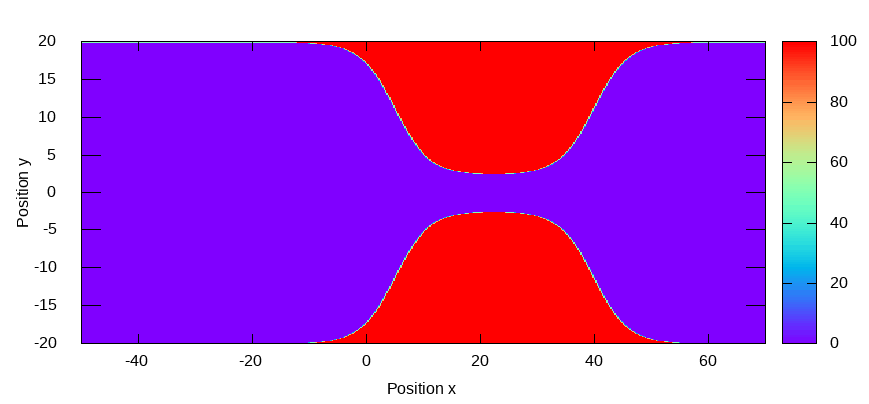
\includegraphics[width=\linewidth]{pot.png}
  \end{subfigure}
  \begin{subfigure}[b]{0.15\linewidth}
    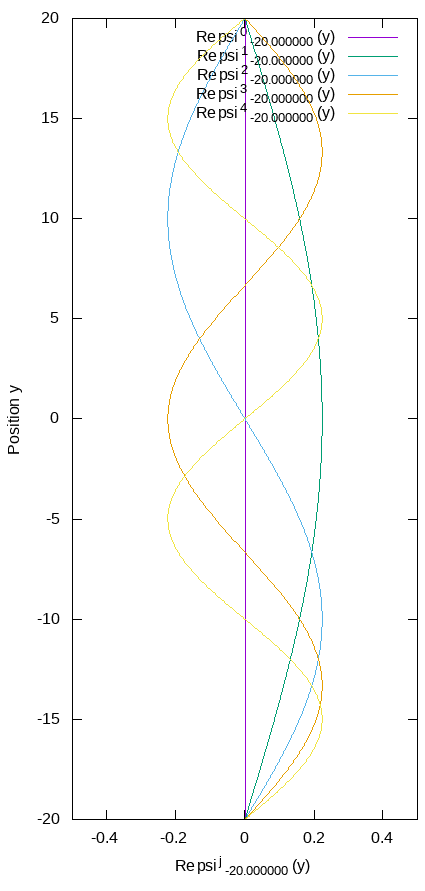
\includegraphics[width=\linewidth]{Eig1.png}
  \end{subfigure}
    \begin{subfigure}[b]{0.15\linewidth}
    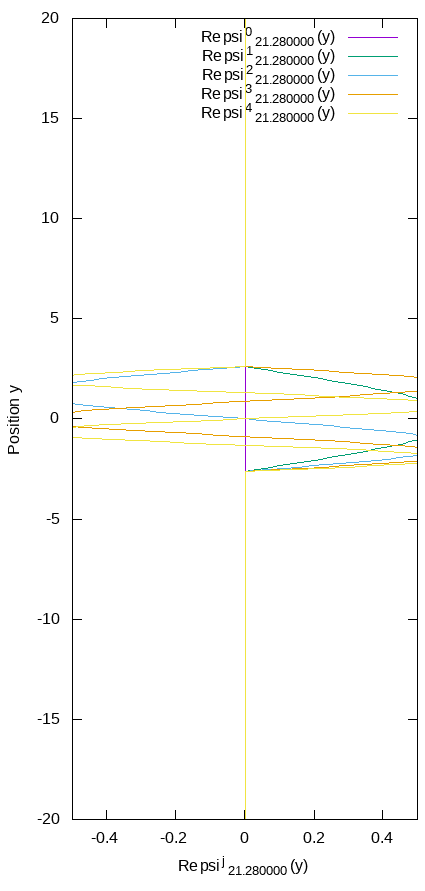
\includegraphics[width=\linewidth]{Eig2.png}
  \end{subfigure}
  \caption{Potential energy profile heatmap in the left and in the center and right respectively, the first non-zero transversal section eigenstates in the broadest and narrowest parts of the set-up.}
  \label{fig:pot}
\end{figure}

The two initial full-wavefunctions we will try are $\Psi(\vec{x},t_0)=GS:=Gauss(x;\mu_x, \sigma_x, k_x)\Phi^1_x(y)$ and $\Psi(\vec{x},t_0)=GG:=Gauss(x; \mu_x, \sigma_x, k_0)Gauss(y; \mu_y, \sigma_y, k_y)$ where $Gauss(x,\mu, \sigma, k_0)$ is a guassian function with standard deviation $\sigma$, expectation $\mu$ and initial momentum $k_0\hbar$:
$$
Gauss(x,\mu,\sigma,k_0)=\sqrt[4]{\frac{1}{2\pi \sigma_x^2}}\ exp\qty(ik_0x-\frac{(x-\mu)^2}{4\sigma^2})
$$
That is, we will analyse the behaviour of: the product of a Gaussian times the first non-zero transversal eigenstate (GS), and the tensor product of two Gaussians (GG), as done in Ref.\cite{Dev}. 

Before jumping to test the approximations, we perform a full wavefunction evolution using no theoretical approximation on the \ref{TDSE}, by employing a 2D Crank Nicolson (CN) method as suggested in Ref.\cite{nireTFGie}. In Figure \ref{fig:population} we can see a heatmap plot of the probability density of both initial conditions, together with the exact adiabatic coefficients for them. Packet (GS) has got exclusive projection on the first transversal eigenstate, which is expected from its definition, while the (GG) requires several odd eigenstates to be expanded (about 3 or 4). Note that by symmetry, the projections on even states are zero.\vspace{-0.3cm}

\begin{figure}[h!]
  \centering
  \begin{subfigure}[b]{0.7\linewidth}
    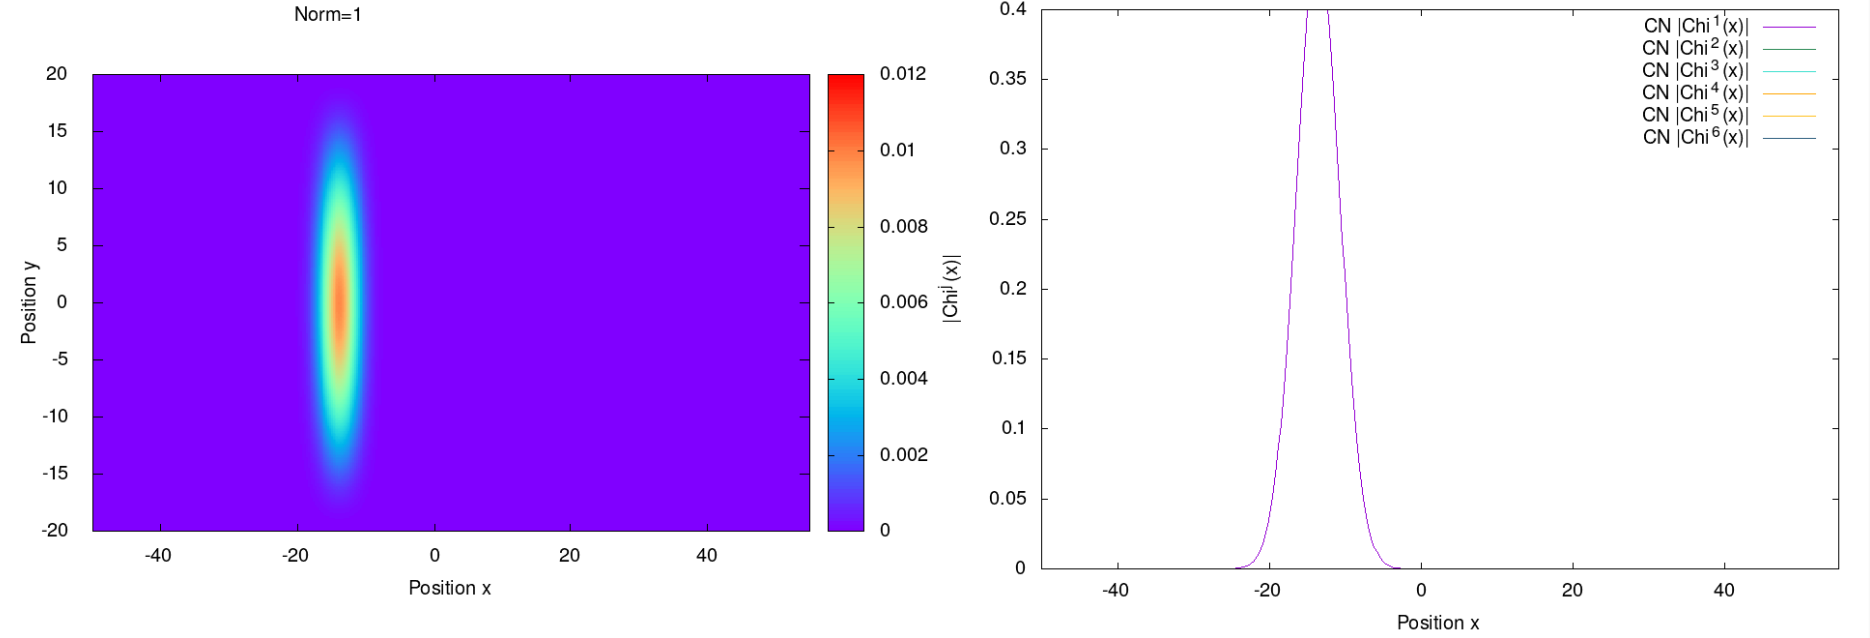
\includegraphics[width=\linewidth]{GS_inik.png}
    \caption{'GS'}
  \end{subfigure}
  \begin{subfigure}[b]{0.7\linewidth}
    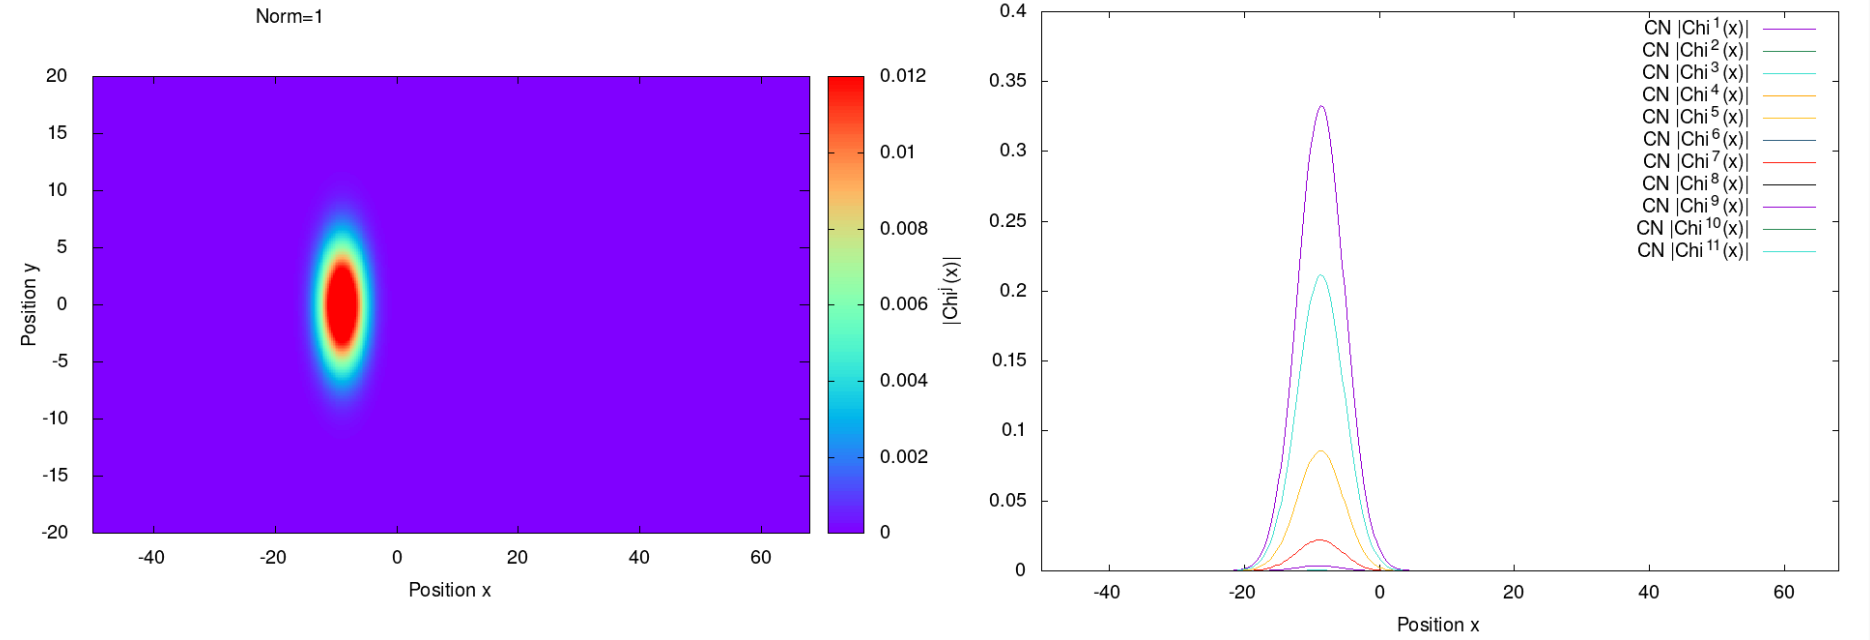
\includegraphics[width=\linewidth]{GG_inik.png}
    \caption{'GG'}
  \end{subfigure}

  \caption{ In the right, the adiabatic state profiles at the initial time and in the left the probability density profile for $GS:=Gauss(x;\mu_x=-14, \sigma_x=2, k_x)\Phi^1_x(y)$ in the left and  $GG:=Gauss(x;\mu_x=-9.5, \sigma_x=2, k_x)Gauss(x;\mu_y=0, \sigma_y=3, k_y)$ in the right. Computed using the full wavefunction evolver CN method.}
  \label{fig:population}
\end{figure}

In Figure \ref{fig:energies} we show the set of initial energies of these wavepackets as a function of their initial momentum, together with the energies of the transversal section eigenstates for $L_{min}=5$ and $L_{min}=8.5$. We see that the GG packet has always a higher initial energy (due to the bigger curvature causing a higher quantum potential). We see that we can choose a wide range of possibilities, from packets with less energy than the ground transversal state to higher than the second transversal eigenstate. 

\begin{figure}[h!]
  \centering
    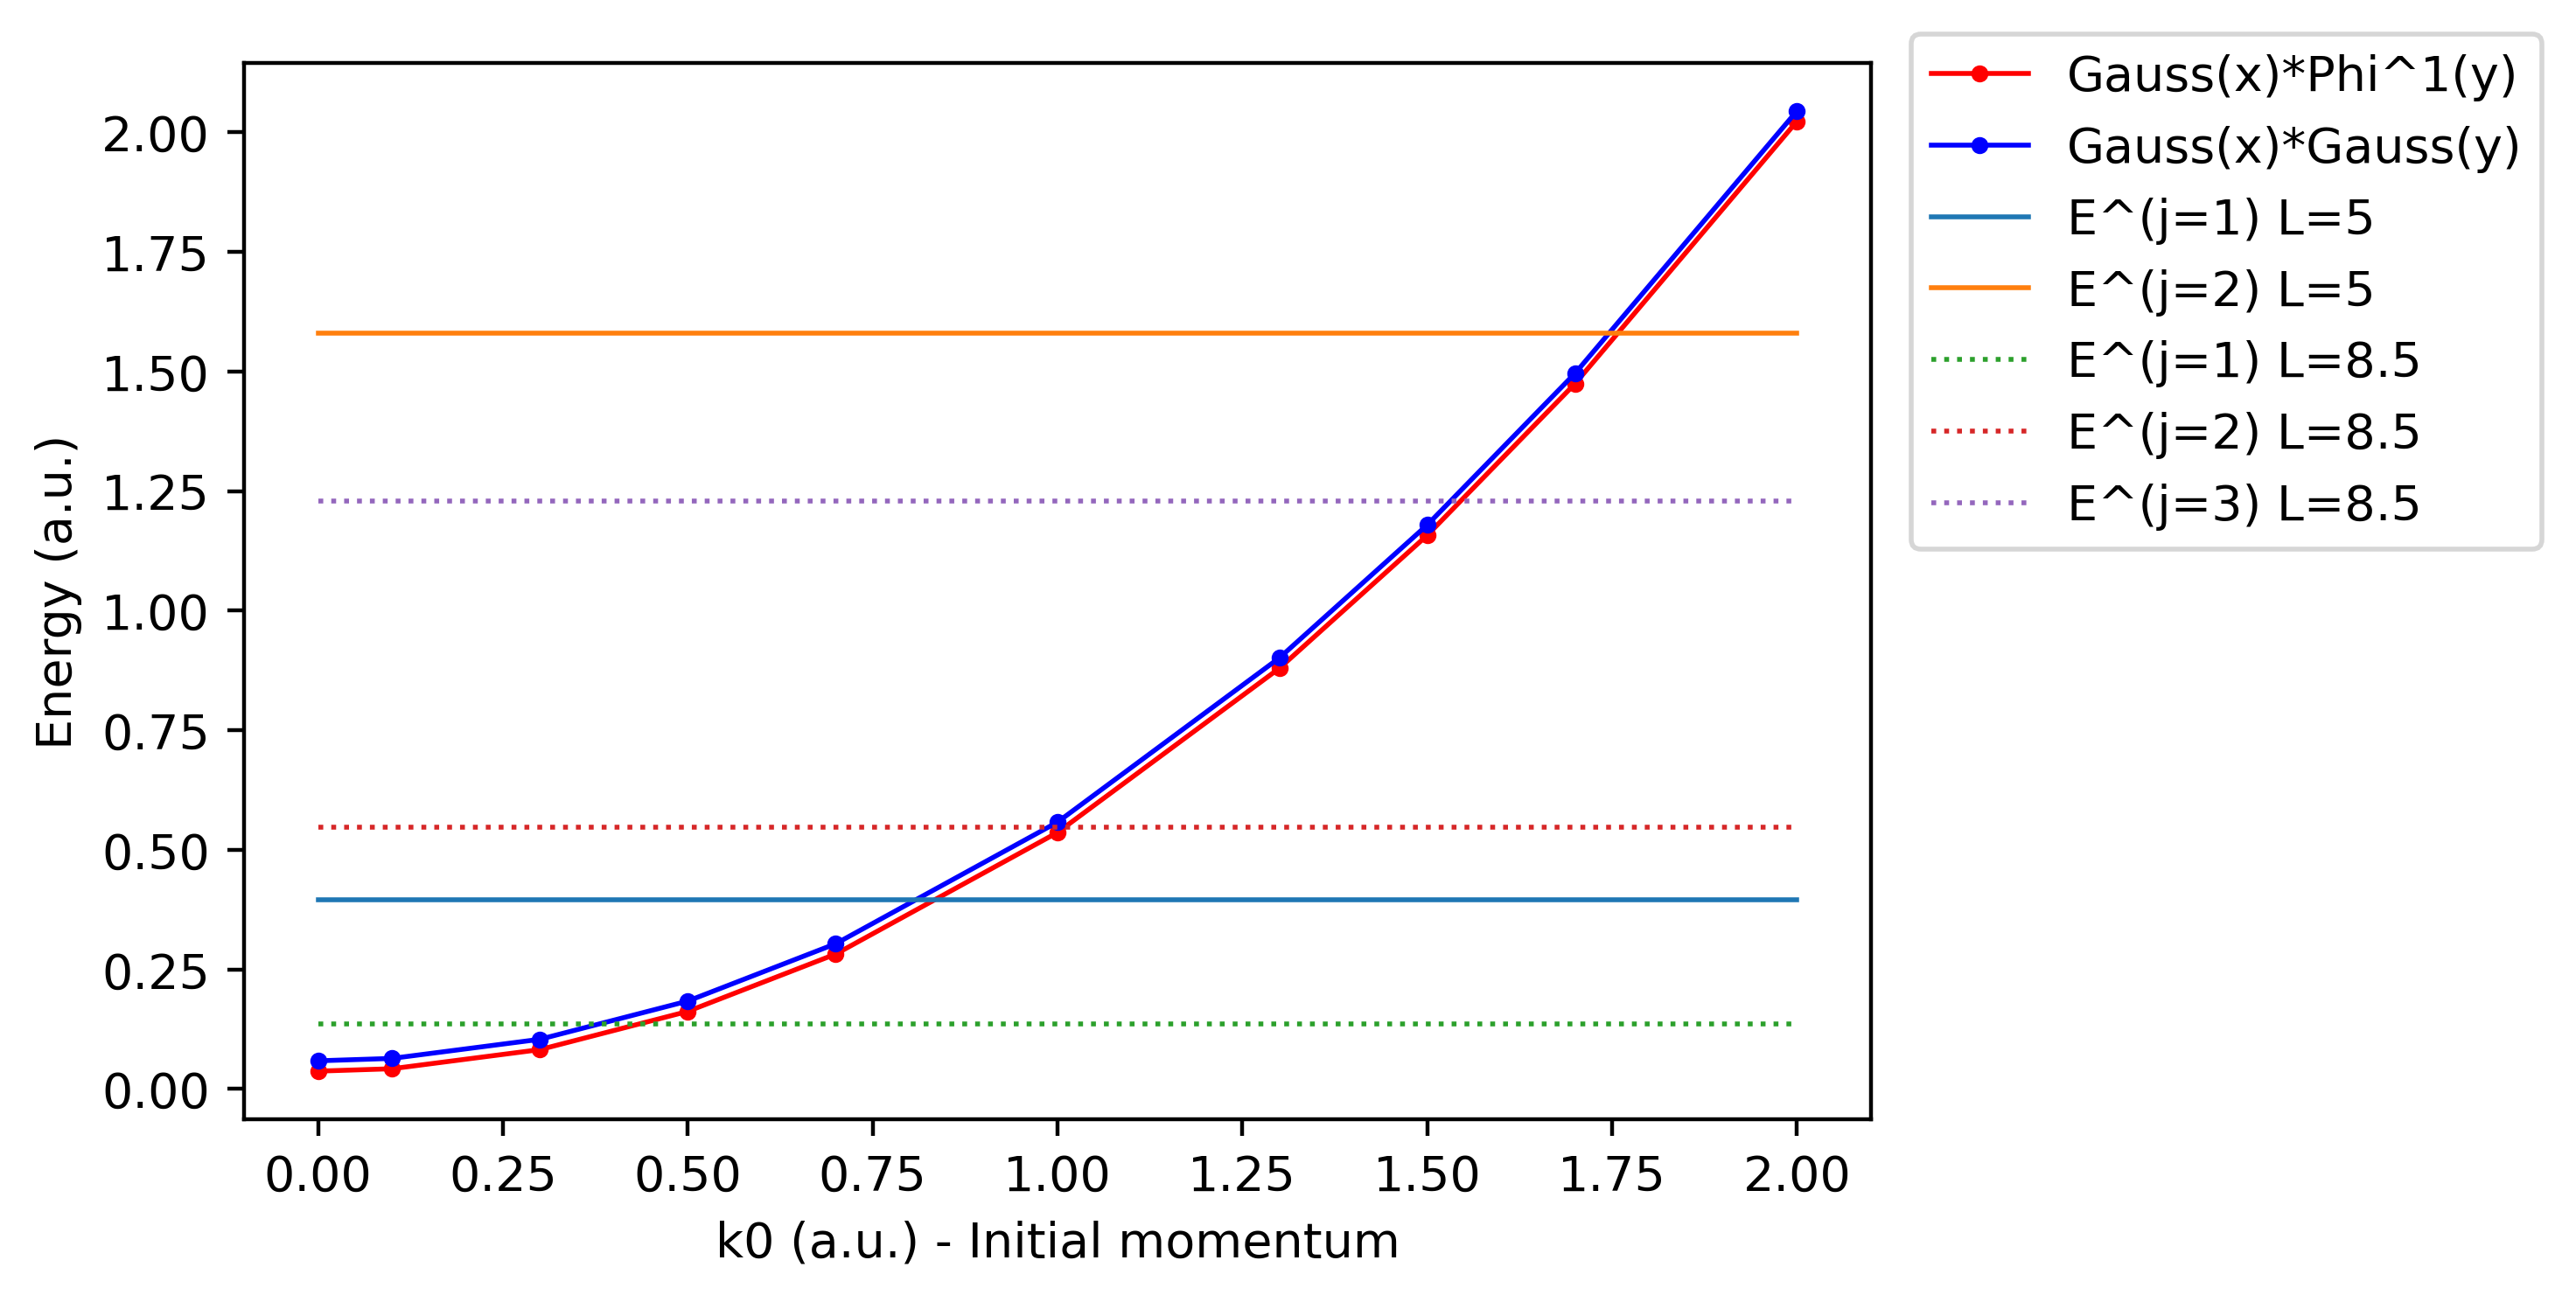
\includegraphics[width=0.7\linewidth]{Evsk_GS_GG_L8_5.png}
  \caption{Average energy in atomic units of $Gauss(x;\mu_x=-14, \sigma_x=2, k_x)\Phi^1_x(y)$ in red and $Gauss(x;\mu_x=-9.5, \sigma_x=2, k_x)Gauss(x;\mu_y=0, \sigma_y=3, k_y)$ in blue as a function of the initial wavepacket momentum for a particle with $m_x=1.0$ and $m_y=0.5$. We can also see in other colours, following the legend, the energy levels of the transversal eigenstates at the narrowest point of the channel, for $L=5$ and $L=8.5$.}
  \label{fig:energies}
\end{figure}


We then choose the range of initial momentums $ k_0 \in [ 0,1 ]$ for both wavepackets as representative enough for the analysis we want to perform. In Figure \ref{fig:popsInTime} we can find the time evolution of the total population of each transversal eigenstate as a function of the initial momentum $k_0$ and for the two different slit widths $L_{min}\in\{5, 8.5\}$. For these same settings, in Figure \ref{fig:CNTransm}, we can find the transmission of the probability density of the full wave-function through the slit in time as a function of the initial momentum $k_0$.\vspace{-0.3cm}

\begin{figure}[h!]
  \centering
  \begin{subfigure}[b]{0.25\linewidth}
    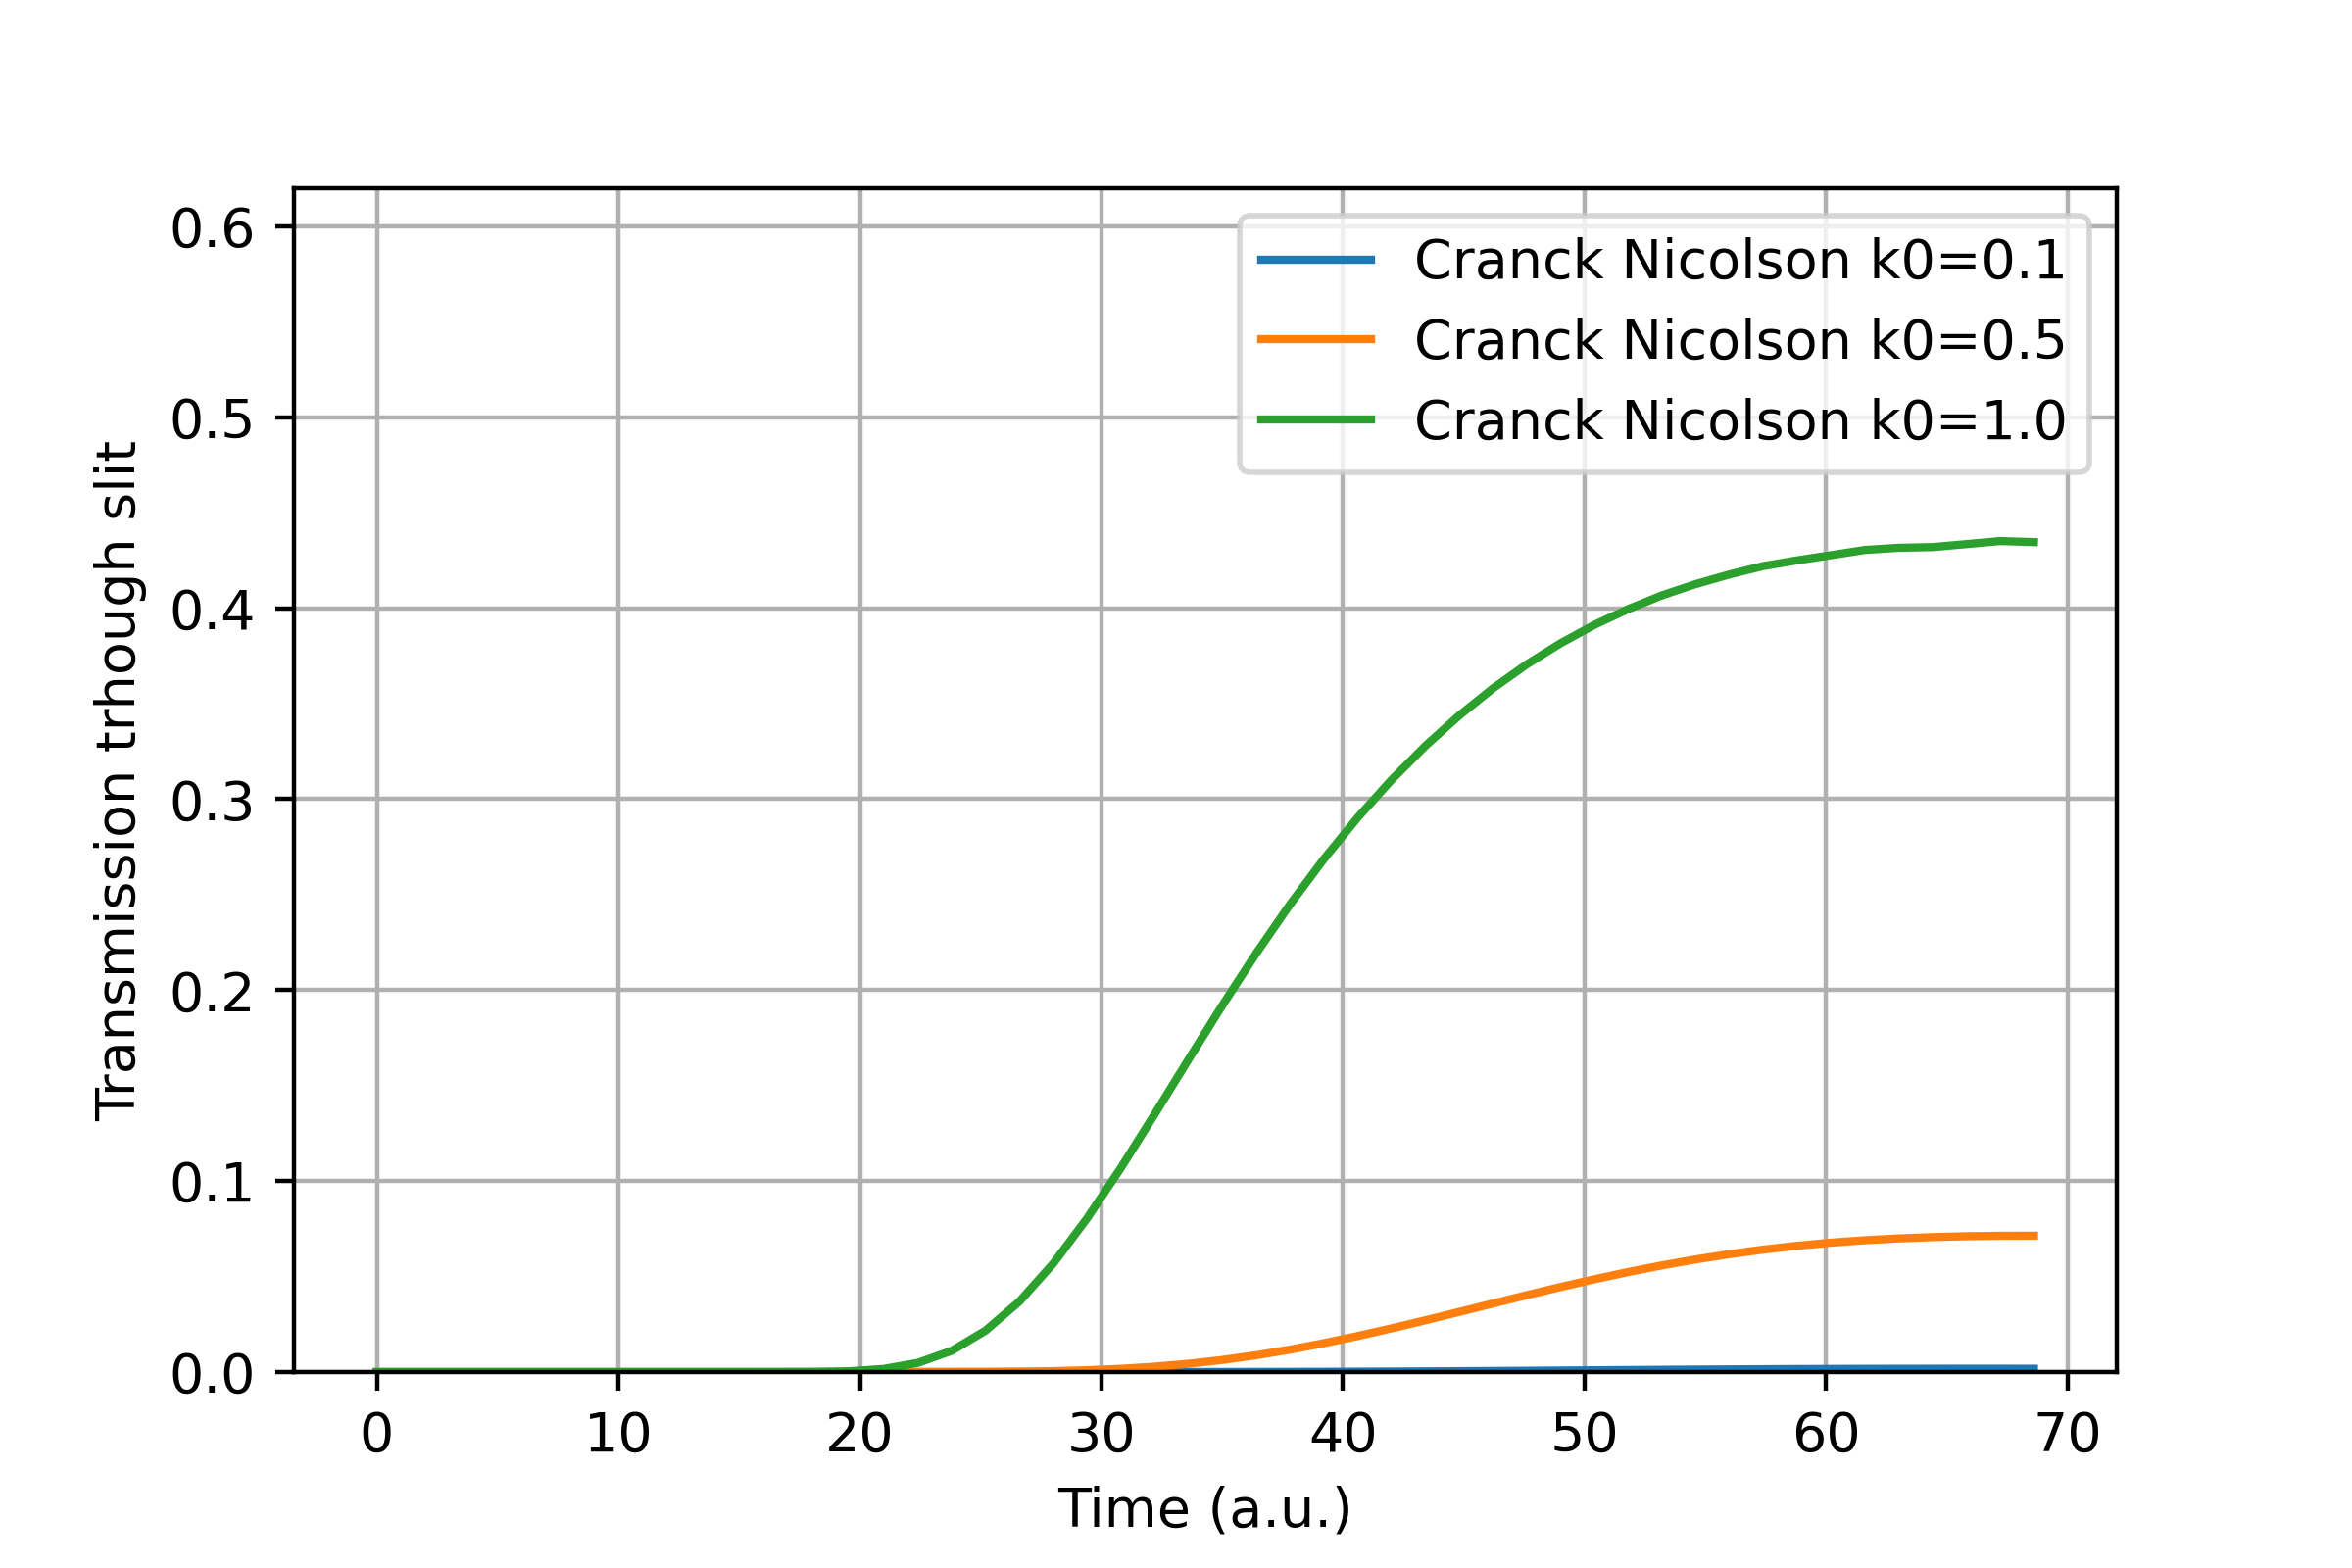
\includegraphics[width=\linewidth]{Transmission_GS_CN_L5.png}
    \caption{GS L=5}
  \end{subfigure}
  \begin{subfigure}[b]{0.24\linewidth}
    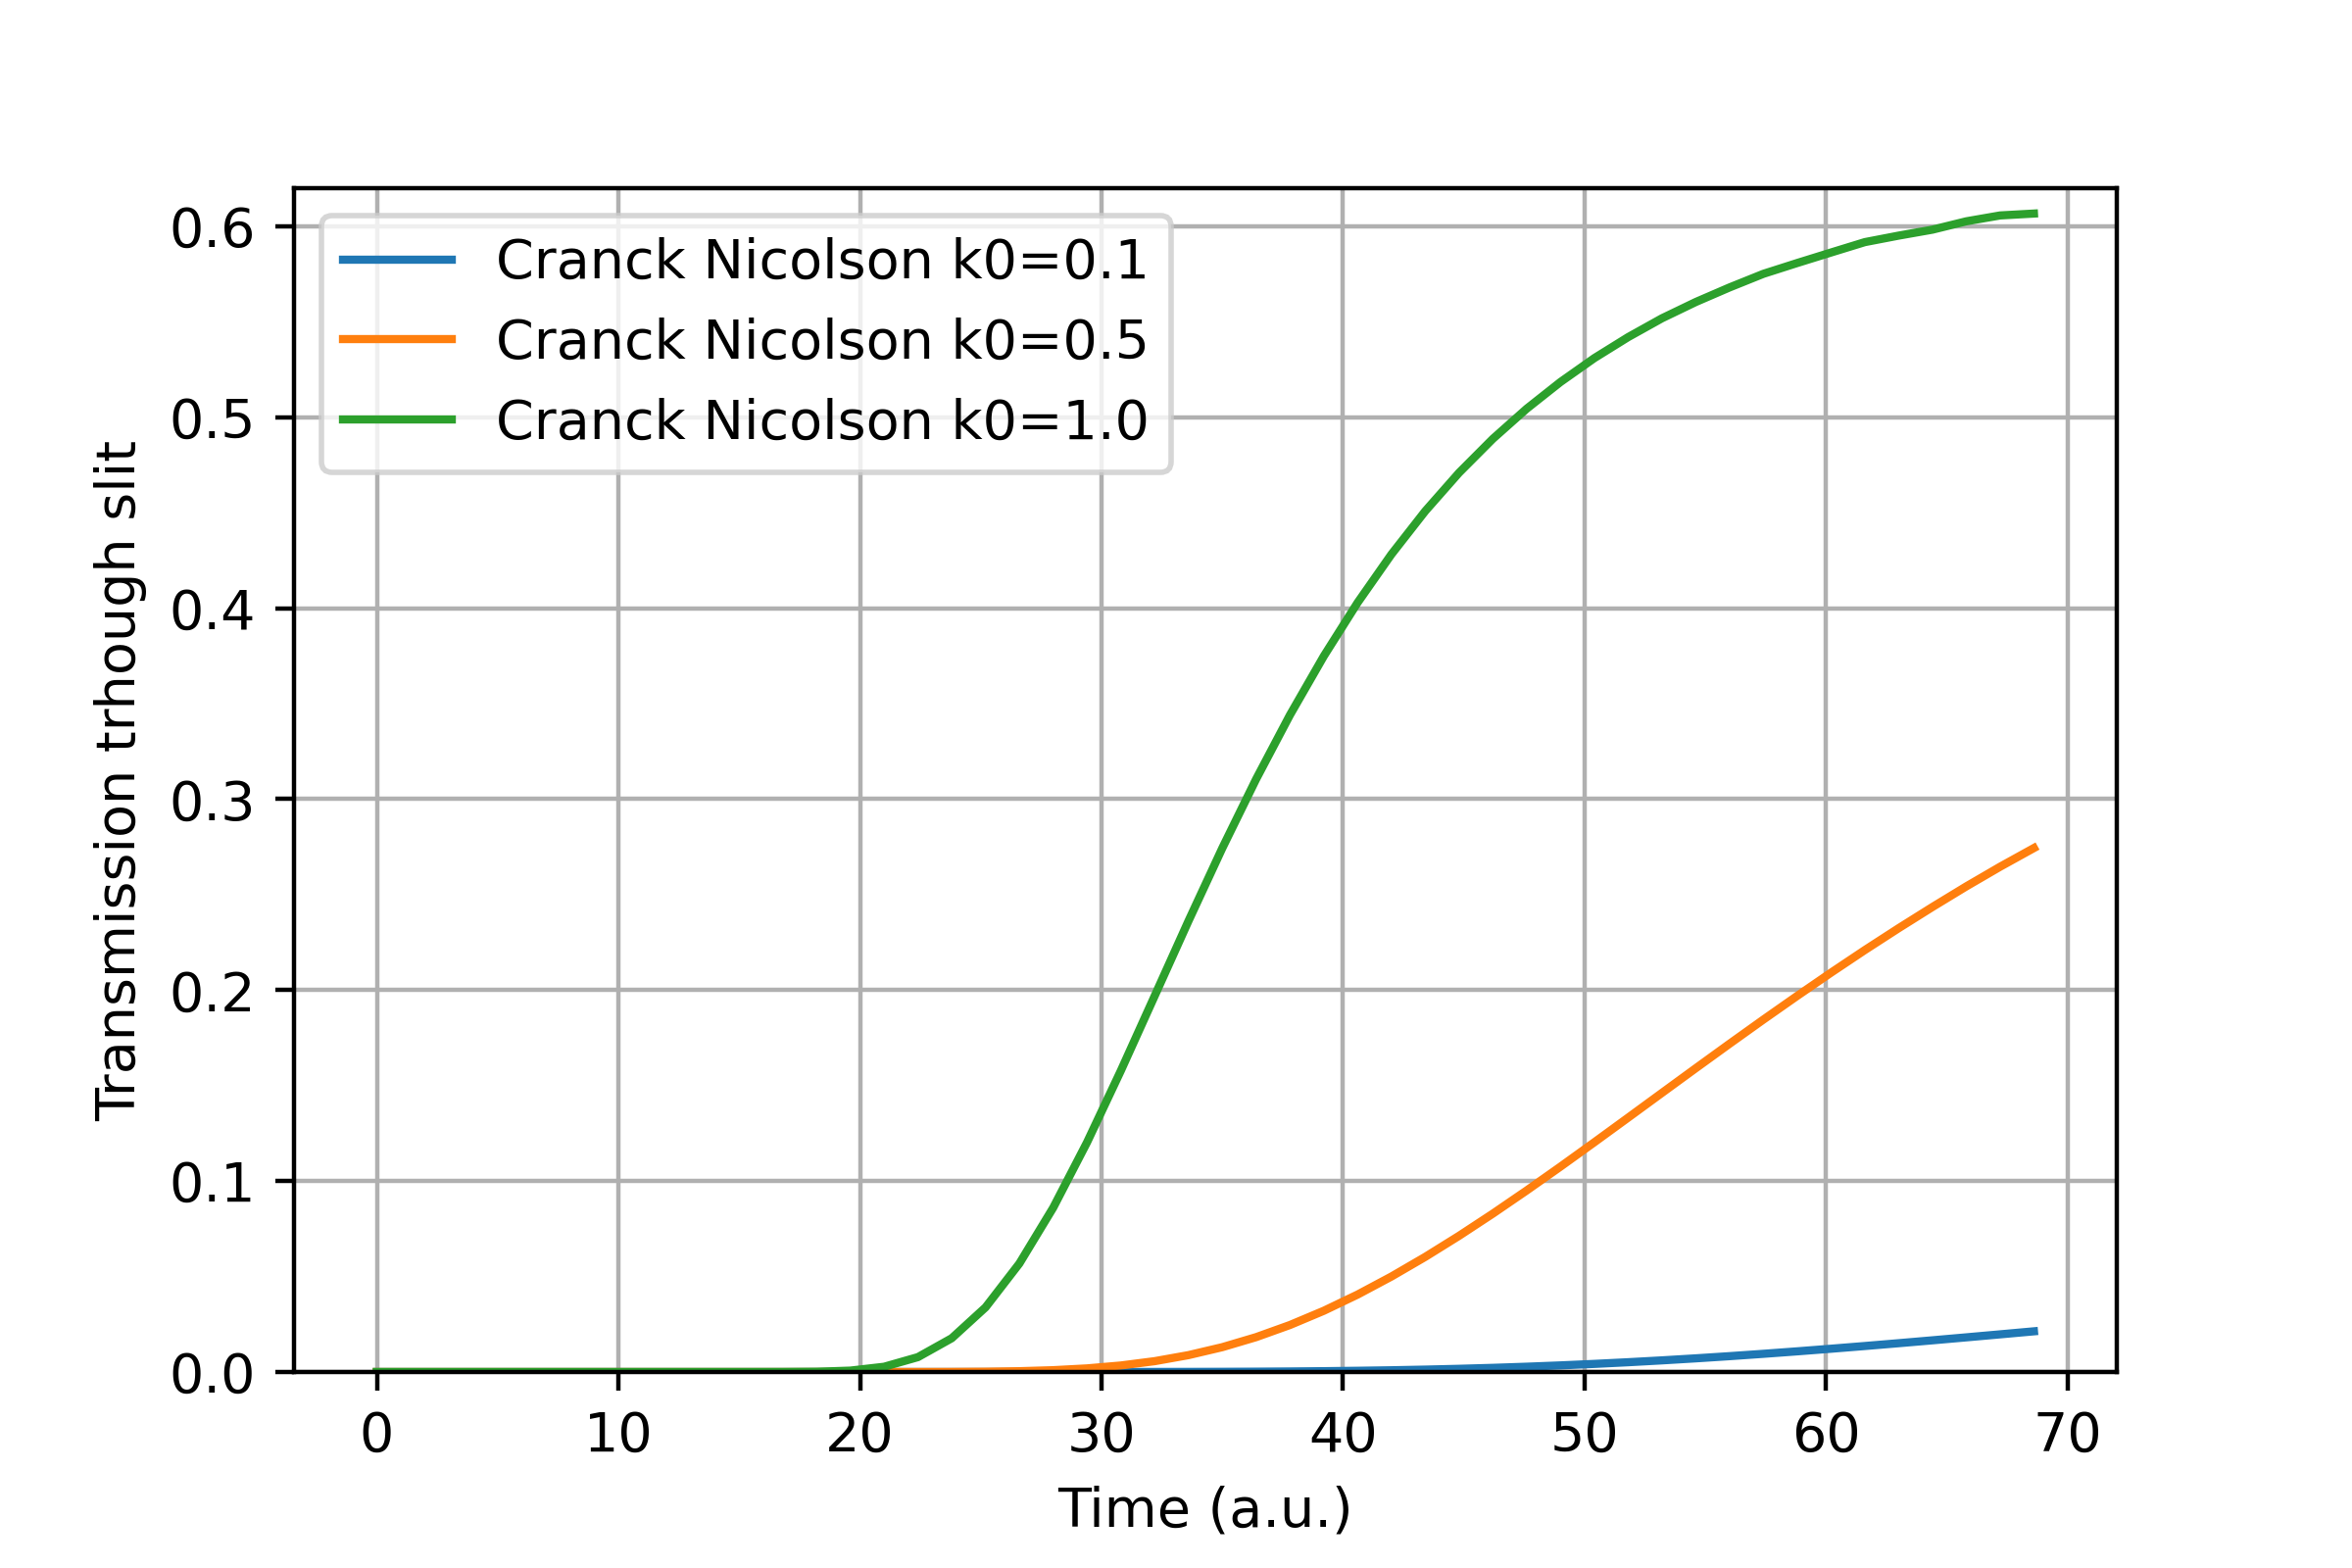
\includegraphics[width=\linewidth]{Transmission_GS_CN_L8.5.png}
    \caption{GS L=8.5}
  \end{subfigure}
    \begin{subfigure}[b]{0.25\linewidth}
    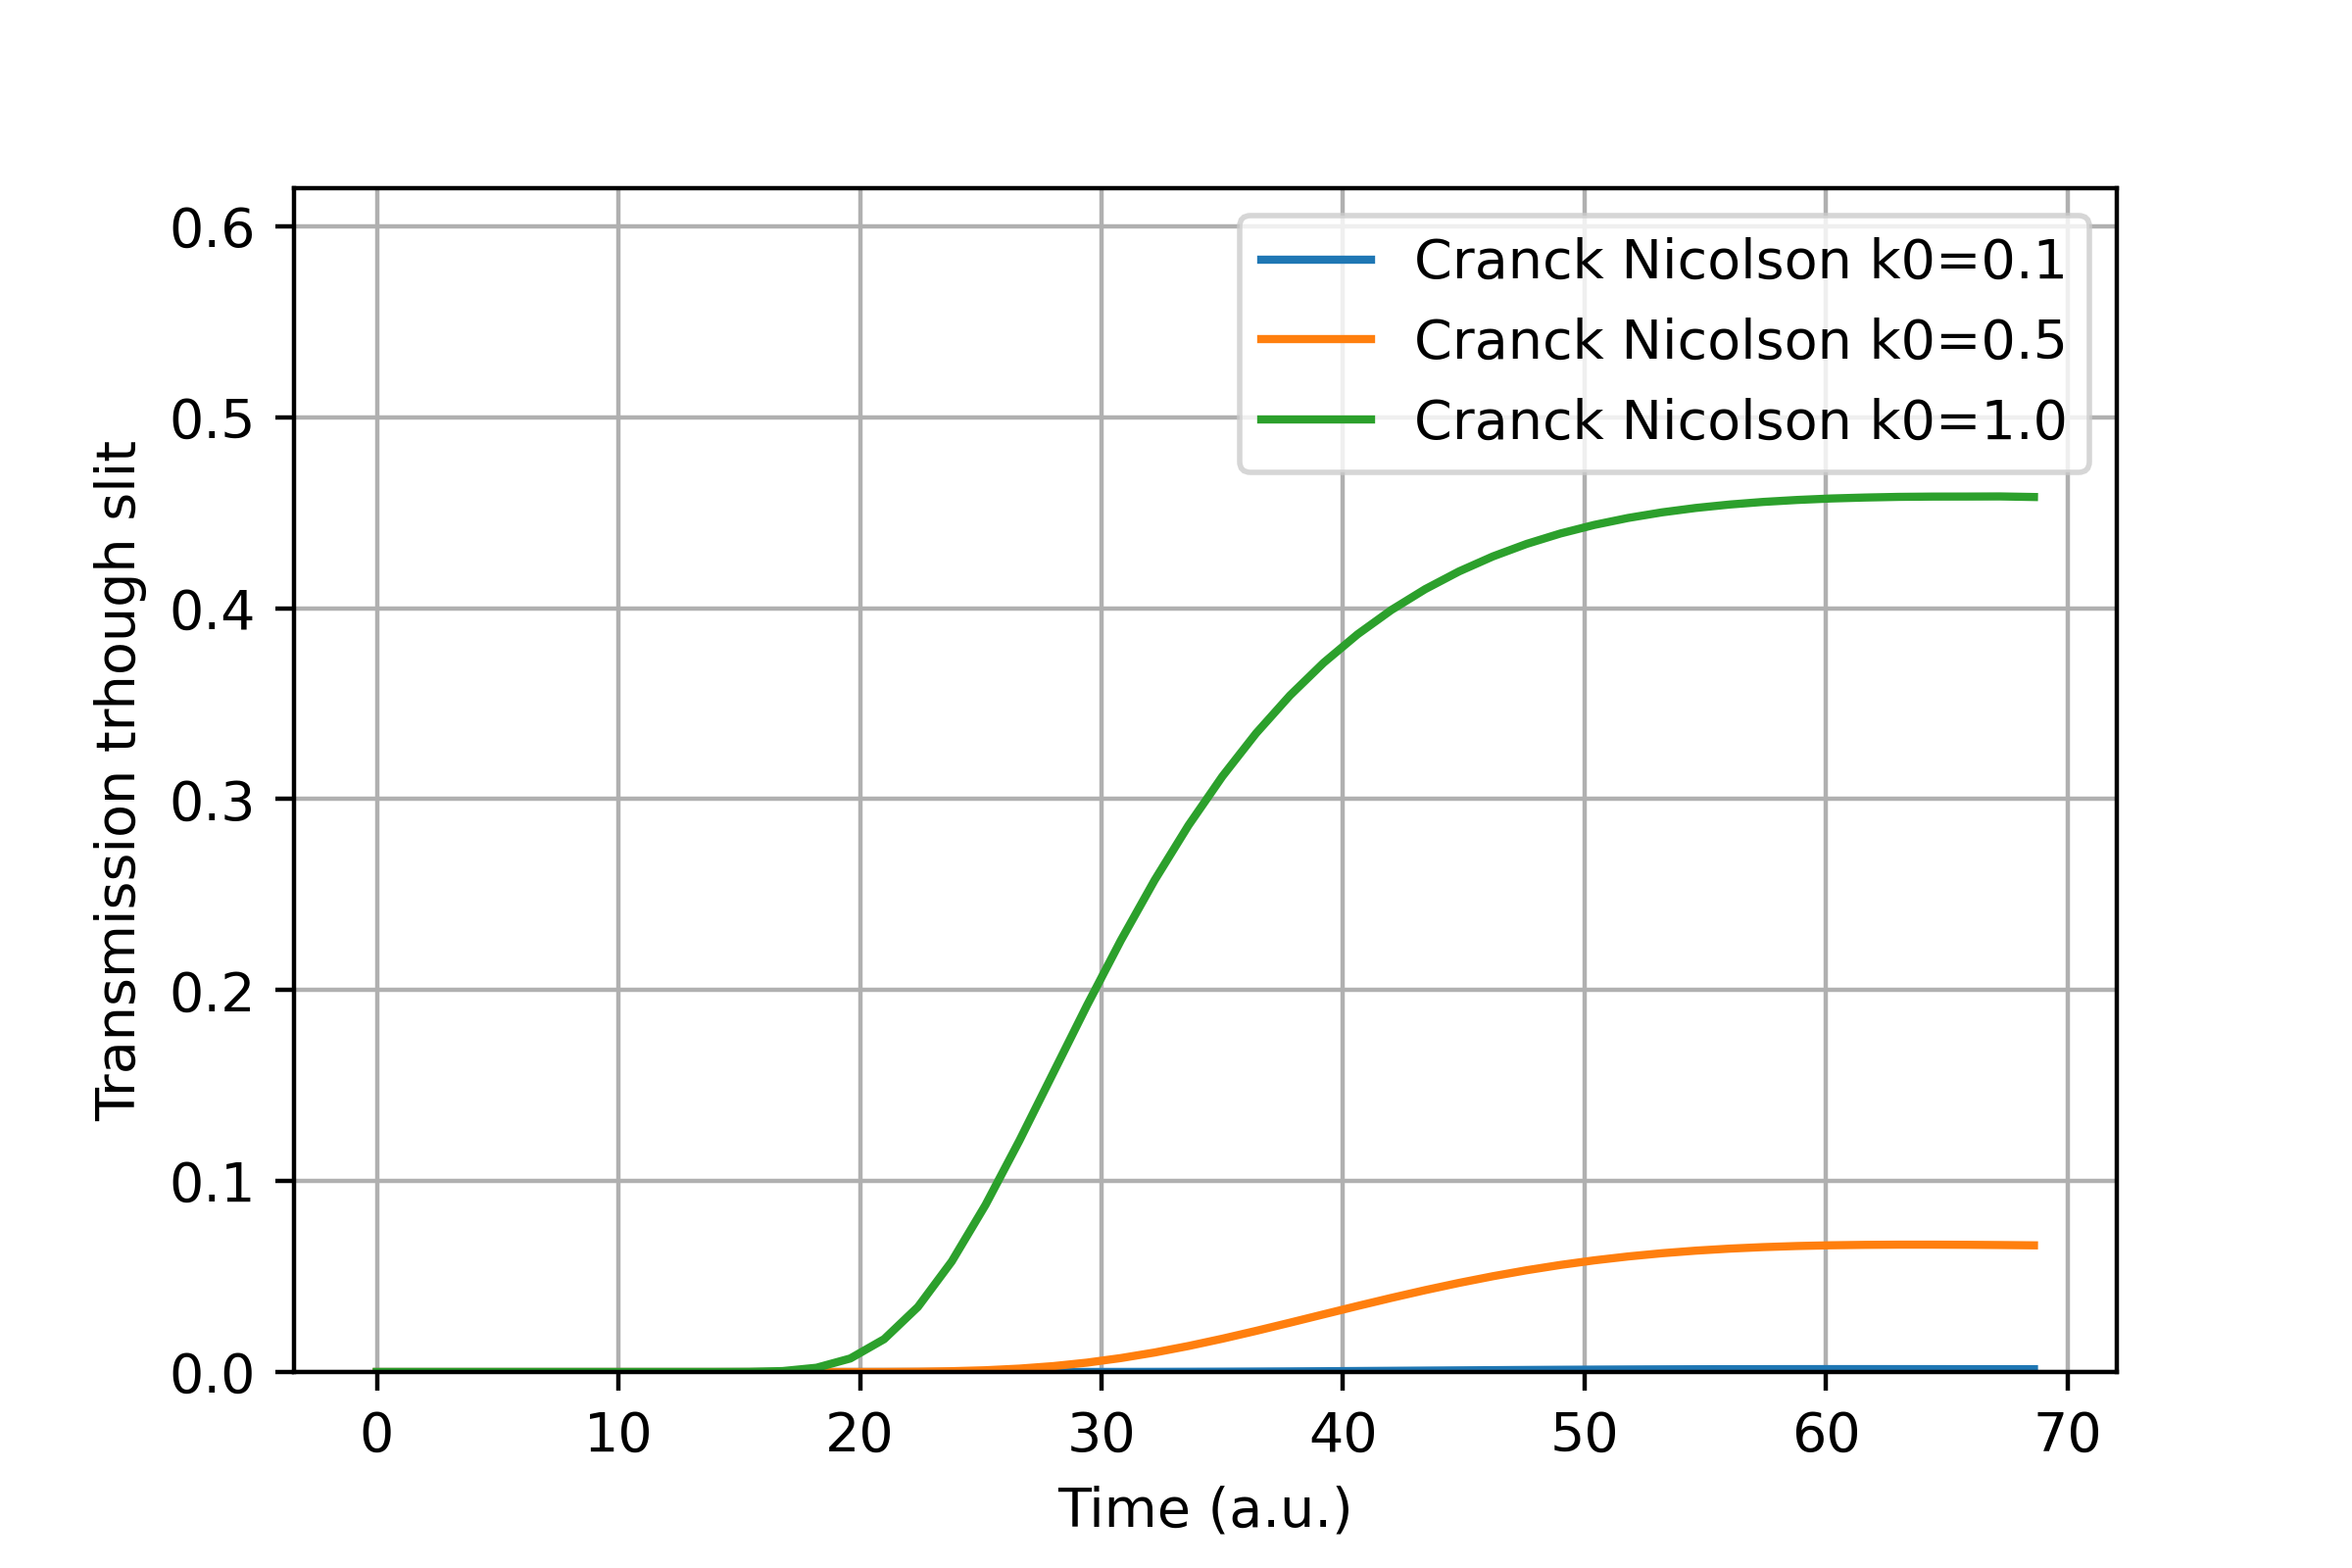
\includegraphics[width=\linewidth]{Transmission_GG_CN_L5.png}
    \caption{GG L=5}
  \end{subfigure}
    \begin{subfigure}[b]{0.24\linewidth}
    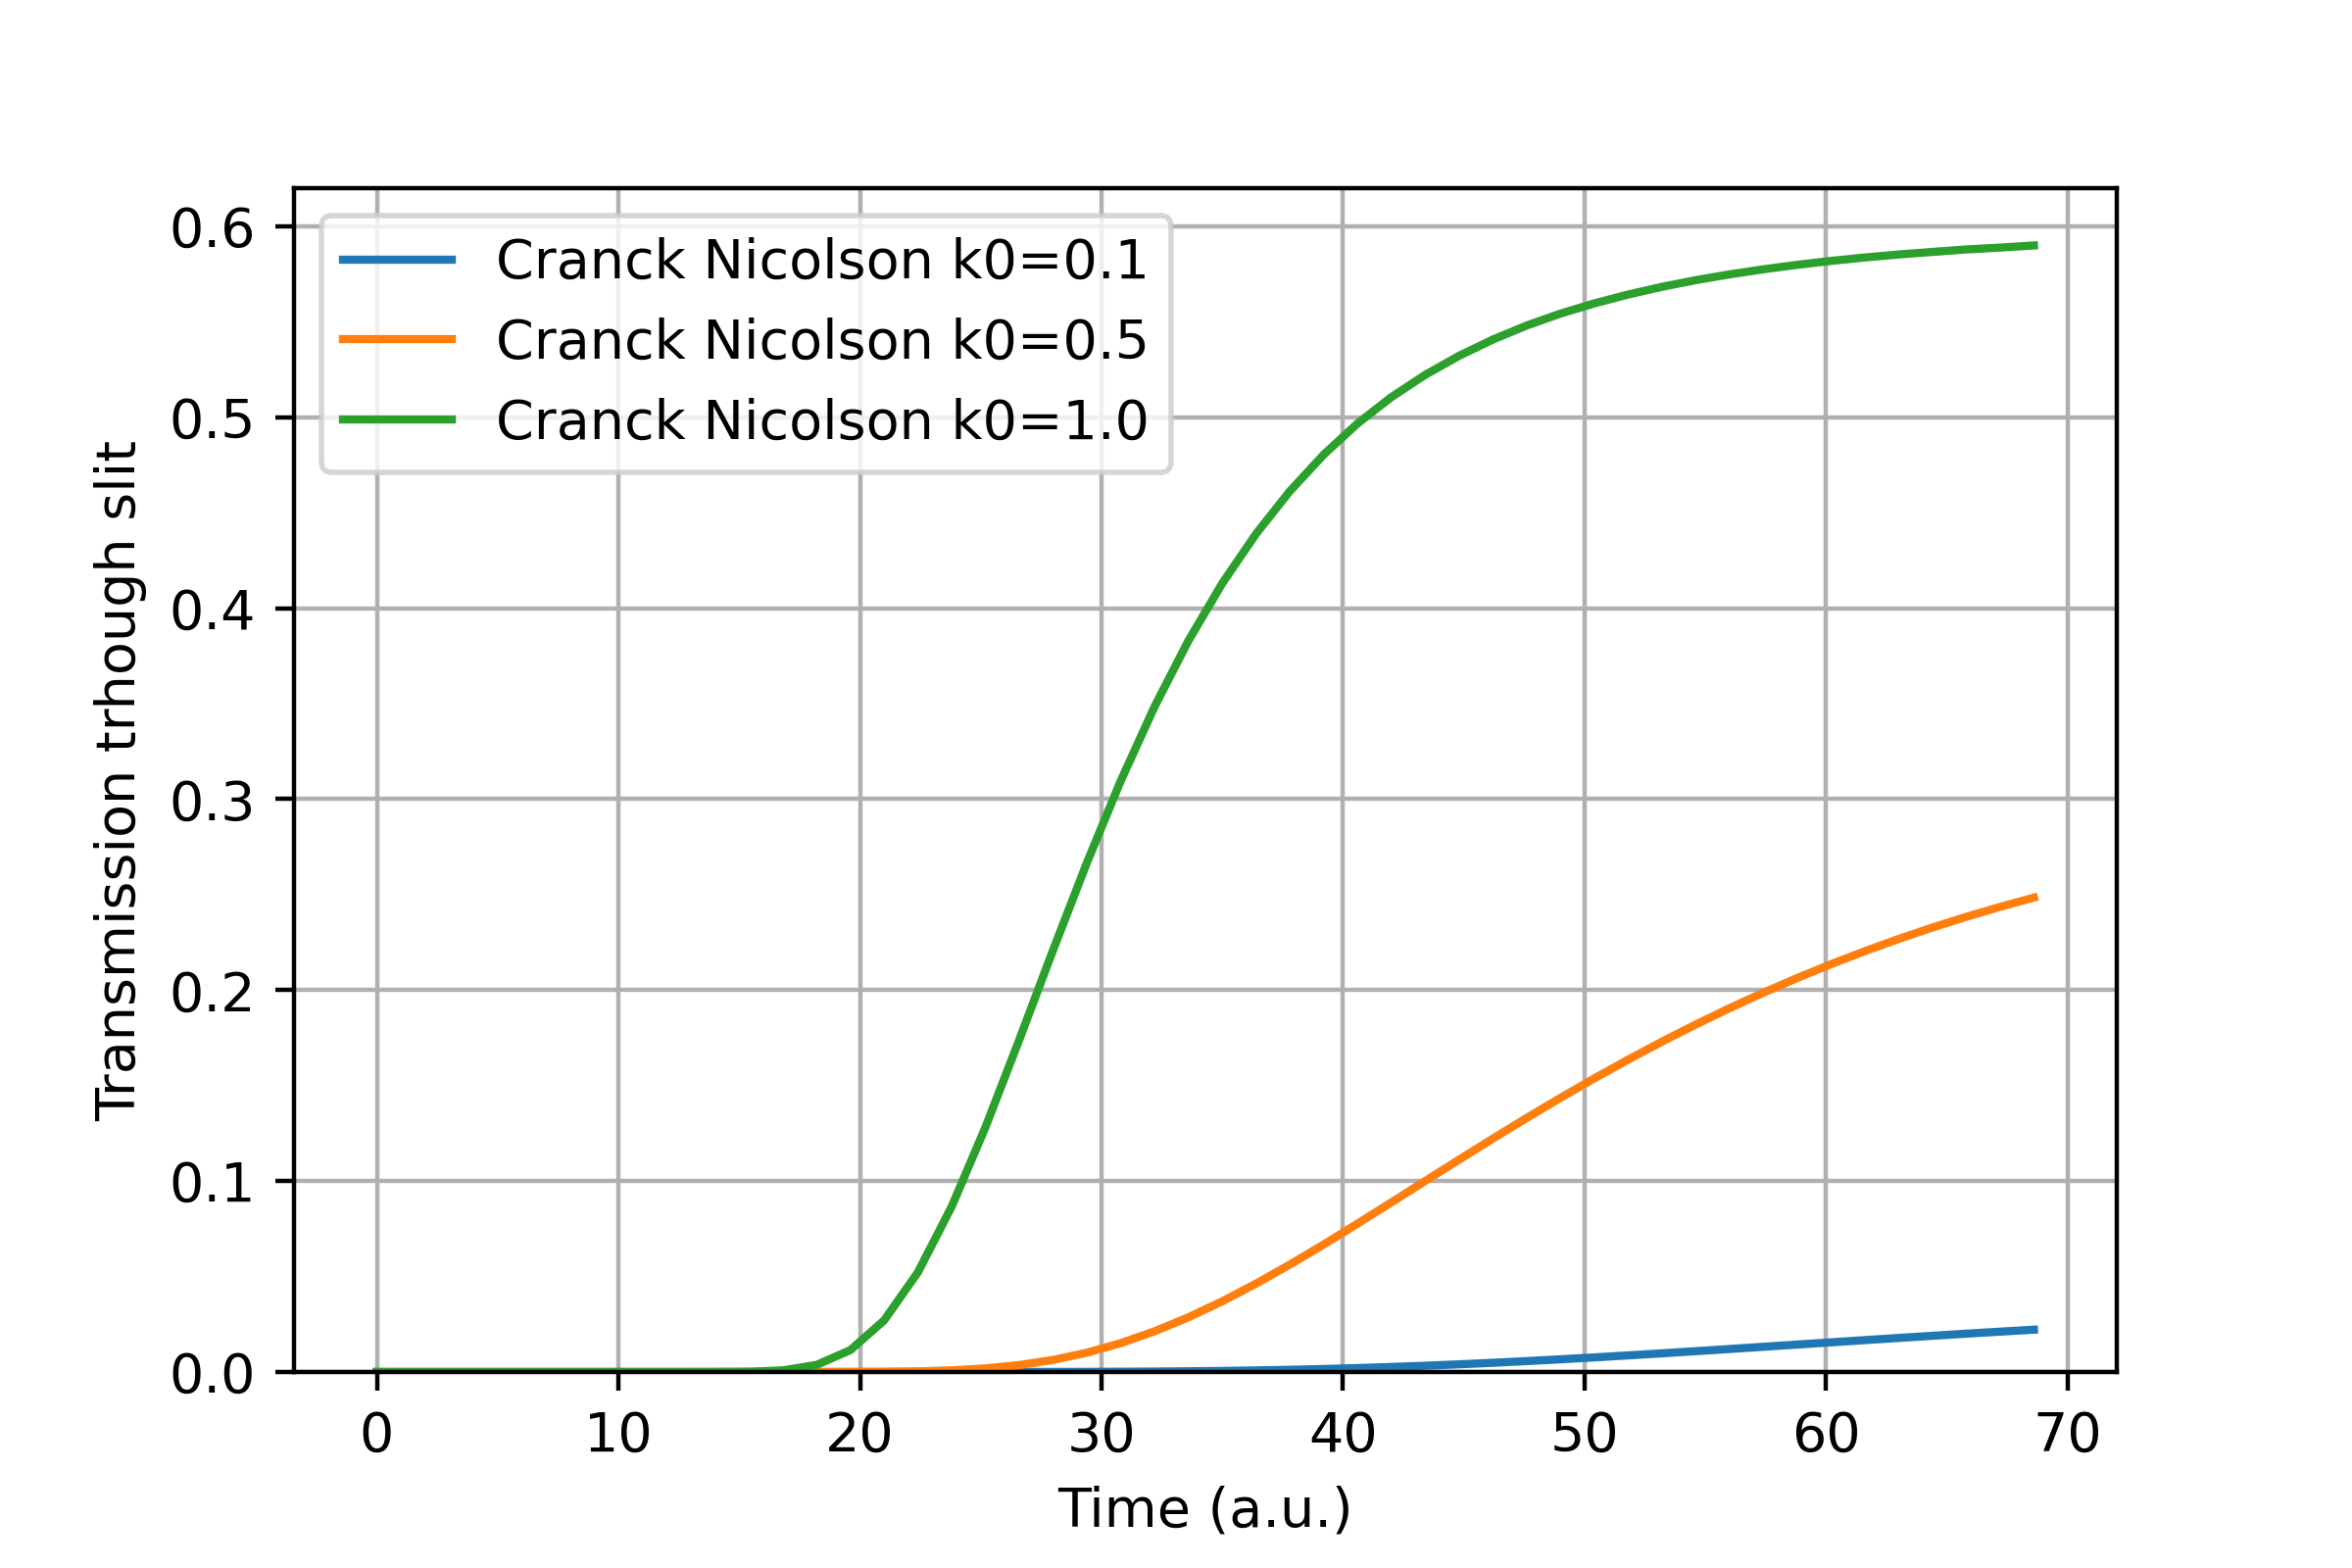
\includegraphics[width=\linewidth]{Transmission_GG_CN_L8.5.png}
    \caption{GG L=8.5}
  \end{subfigure}

  \caption{ Transmission of the full wavefunction probability density through the slit as a function of time. Computed using the CN method. $GS:=Gauss(x;\mu_x, \sigma_x, k_x)\Phi^1_x(y)$, while $GG:=Gauss(x;\mu_x, \sigma_x, k_x)Gauss(x;\mu_y, \sigma_y, k_y)$.\vspace{-0.25cm}}
  \label{fig:CNTransm}
\end{figure}

\begin{figure}[h!]
  \centering
  \begin{subfigure}[b]{0.36\linewidth}
    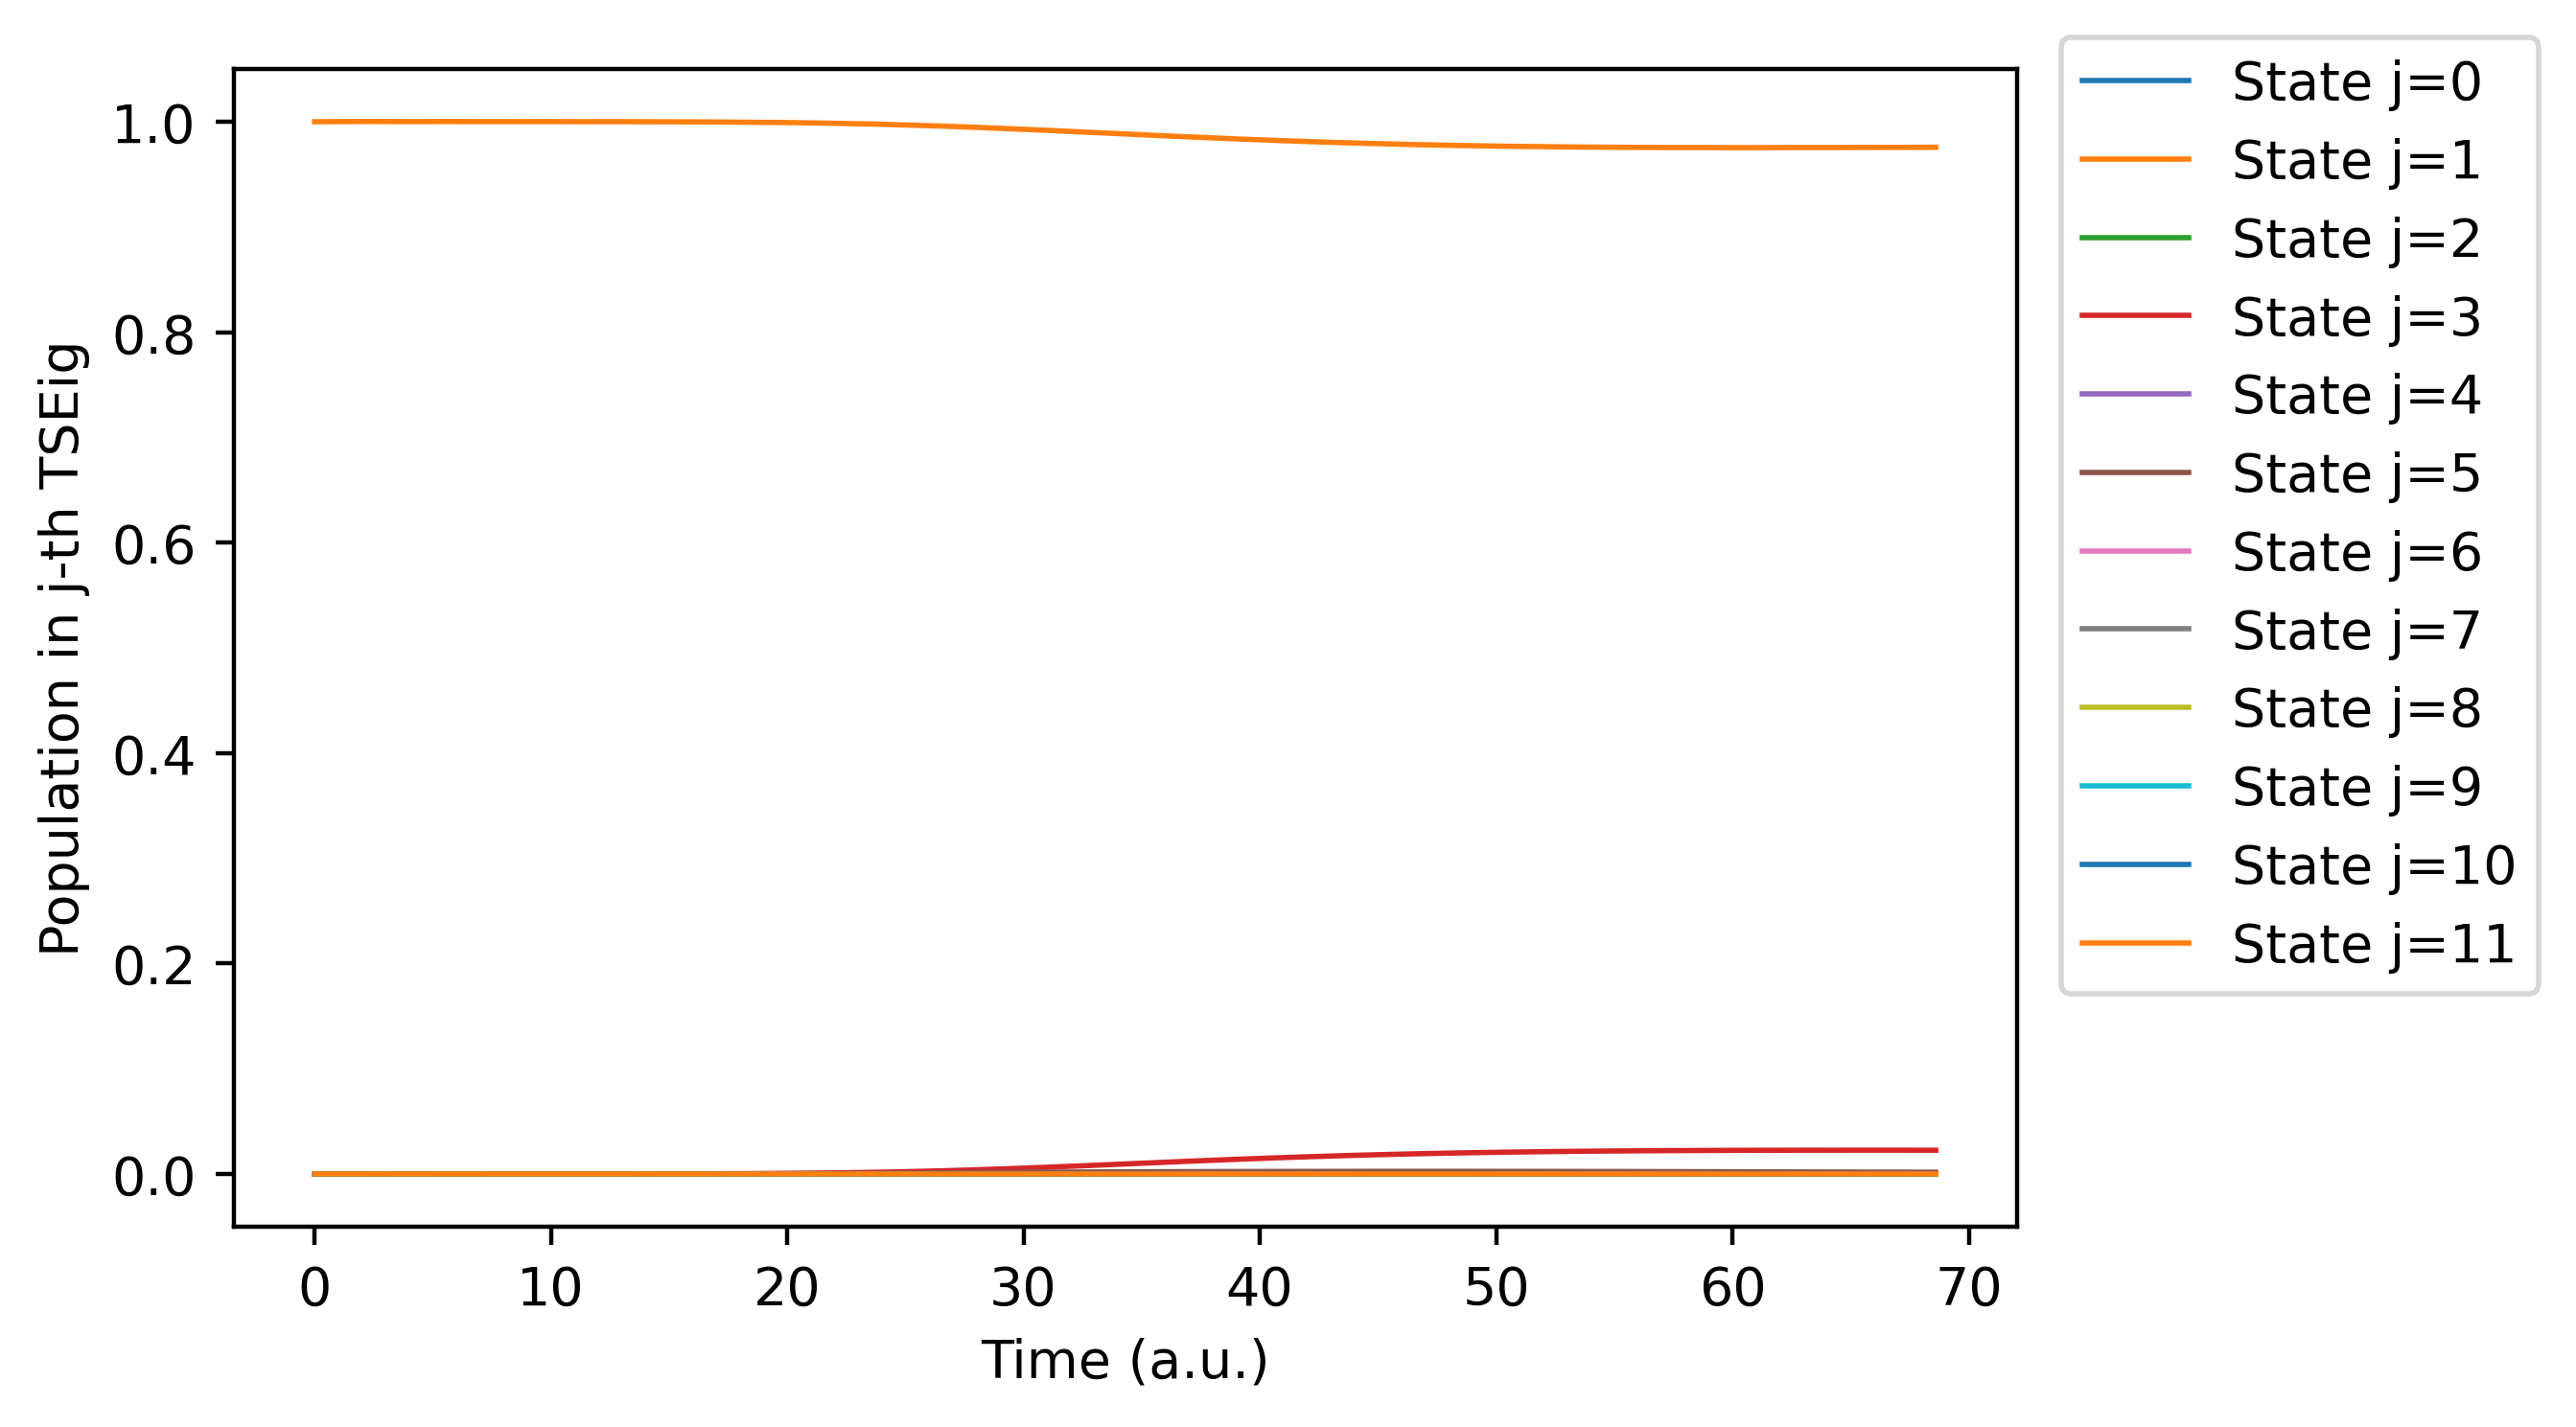
\includegraphics[width=\linewidth]{Population_GS_L5_k0_0.1.png}
    \caption{GS L=5 k=0.1}
  \end{subfigure}
    \begin{subfigure}[b]{0.30\linewidth}
    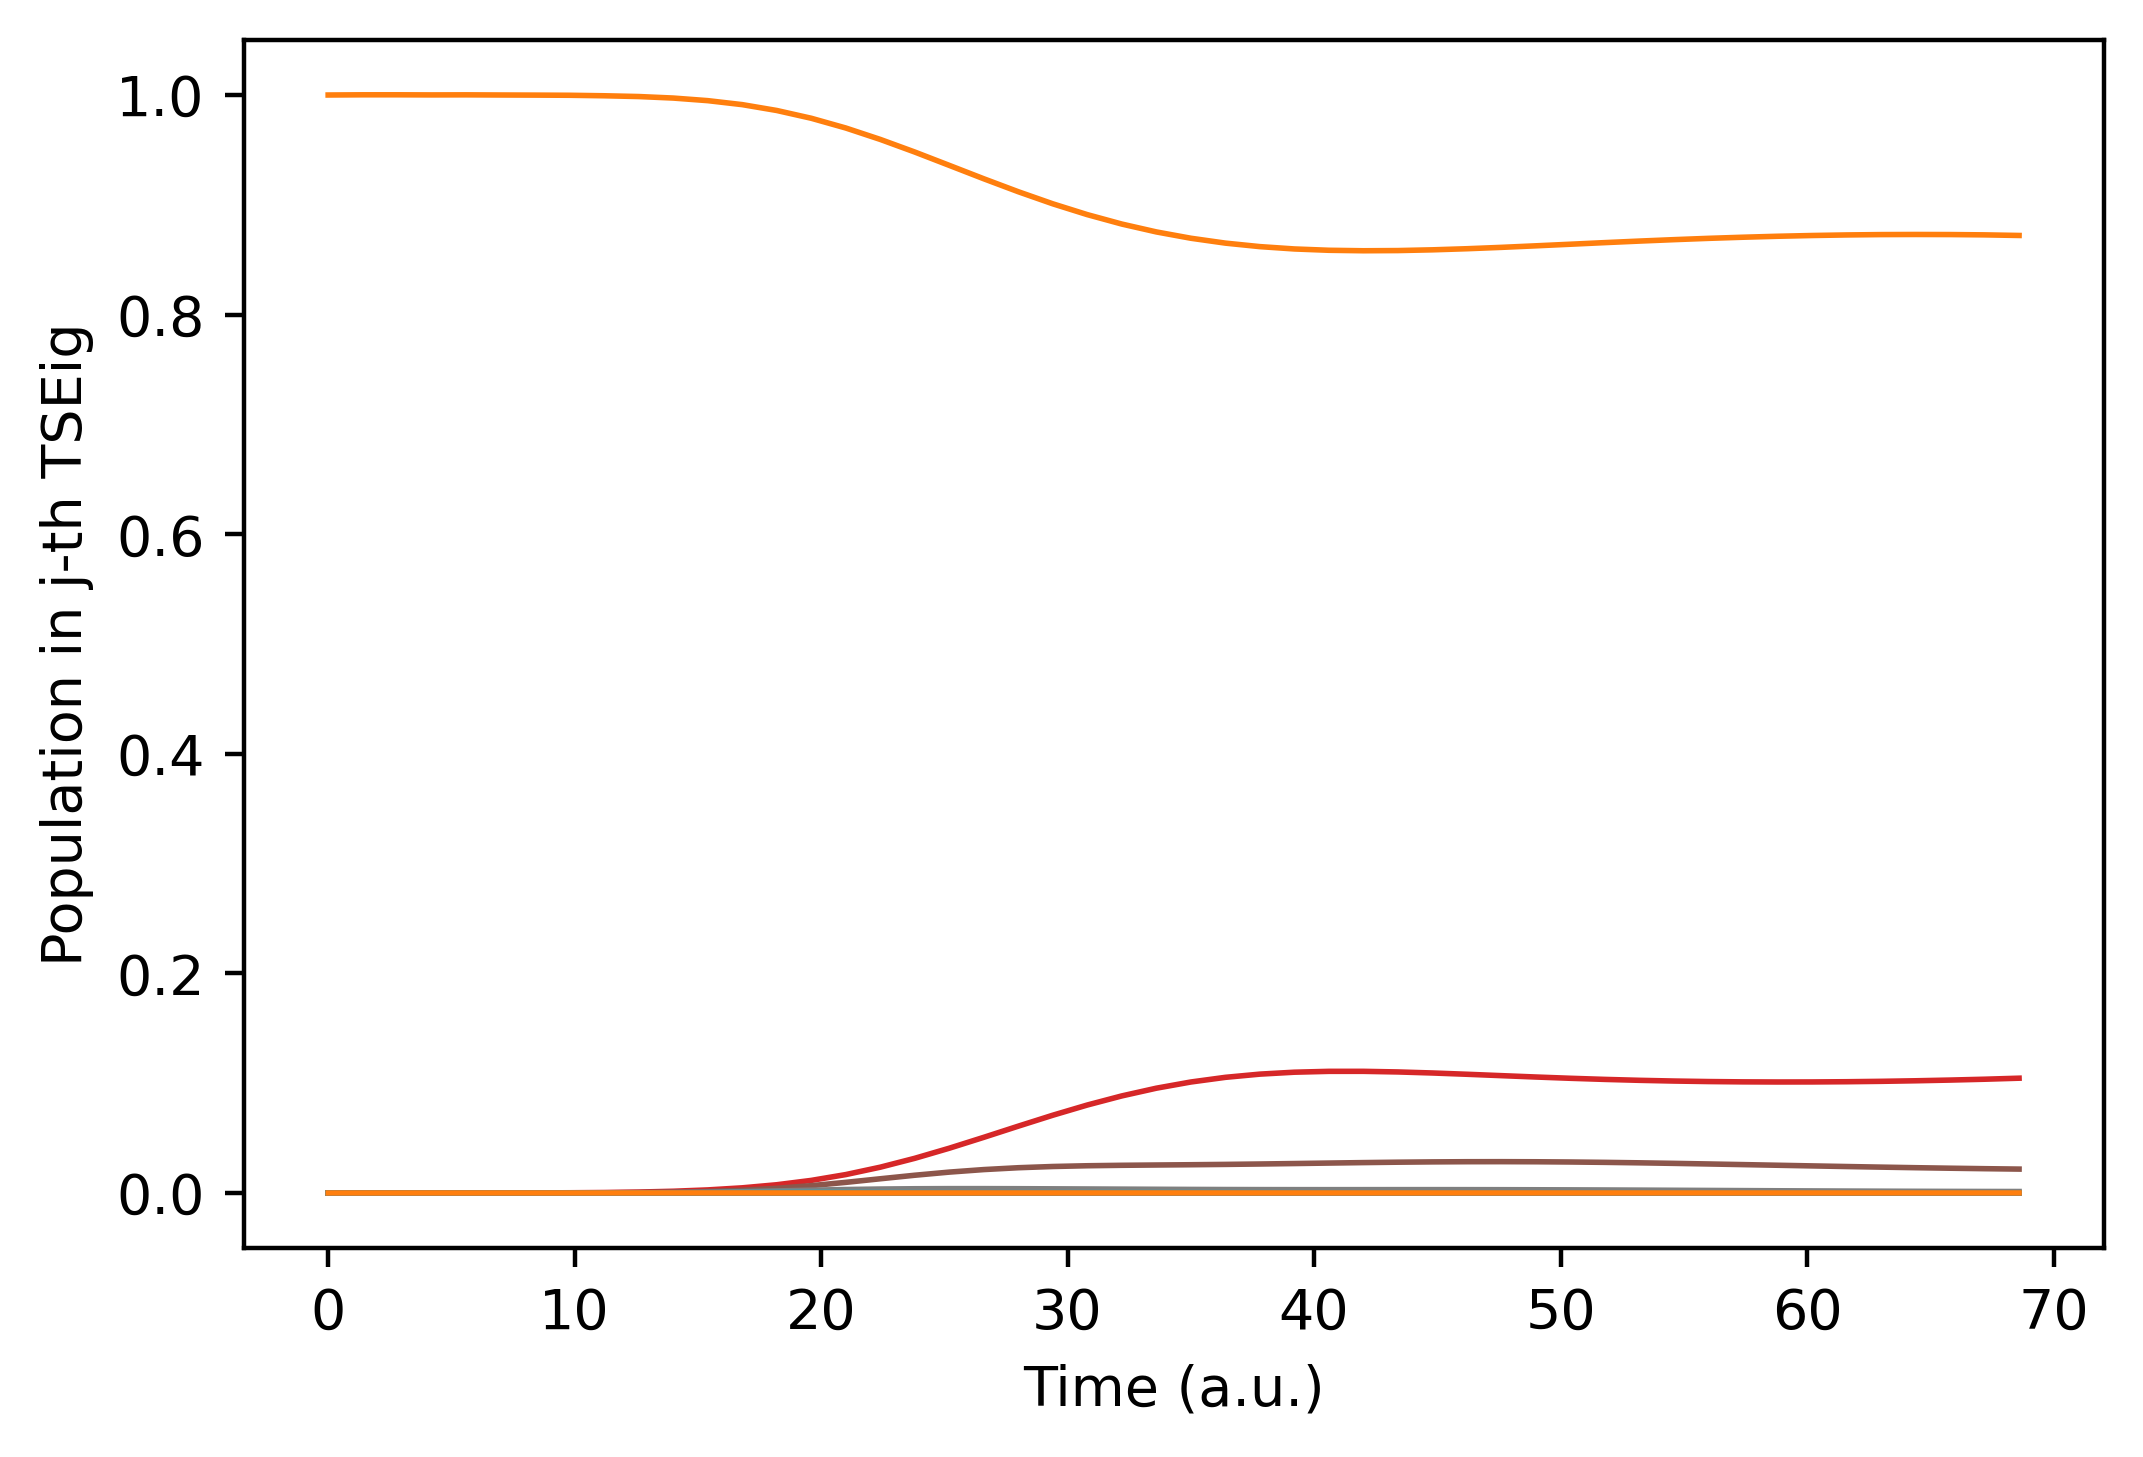
\includegraphics[width=\linewidth]{Population_GS_L5_k0_0.5.png}
    \caption{GS L=5 k=0.5}
  \end{subfigure}  
  \begin{subfigure}[b]{0.30\linewidth}
    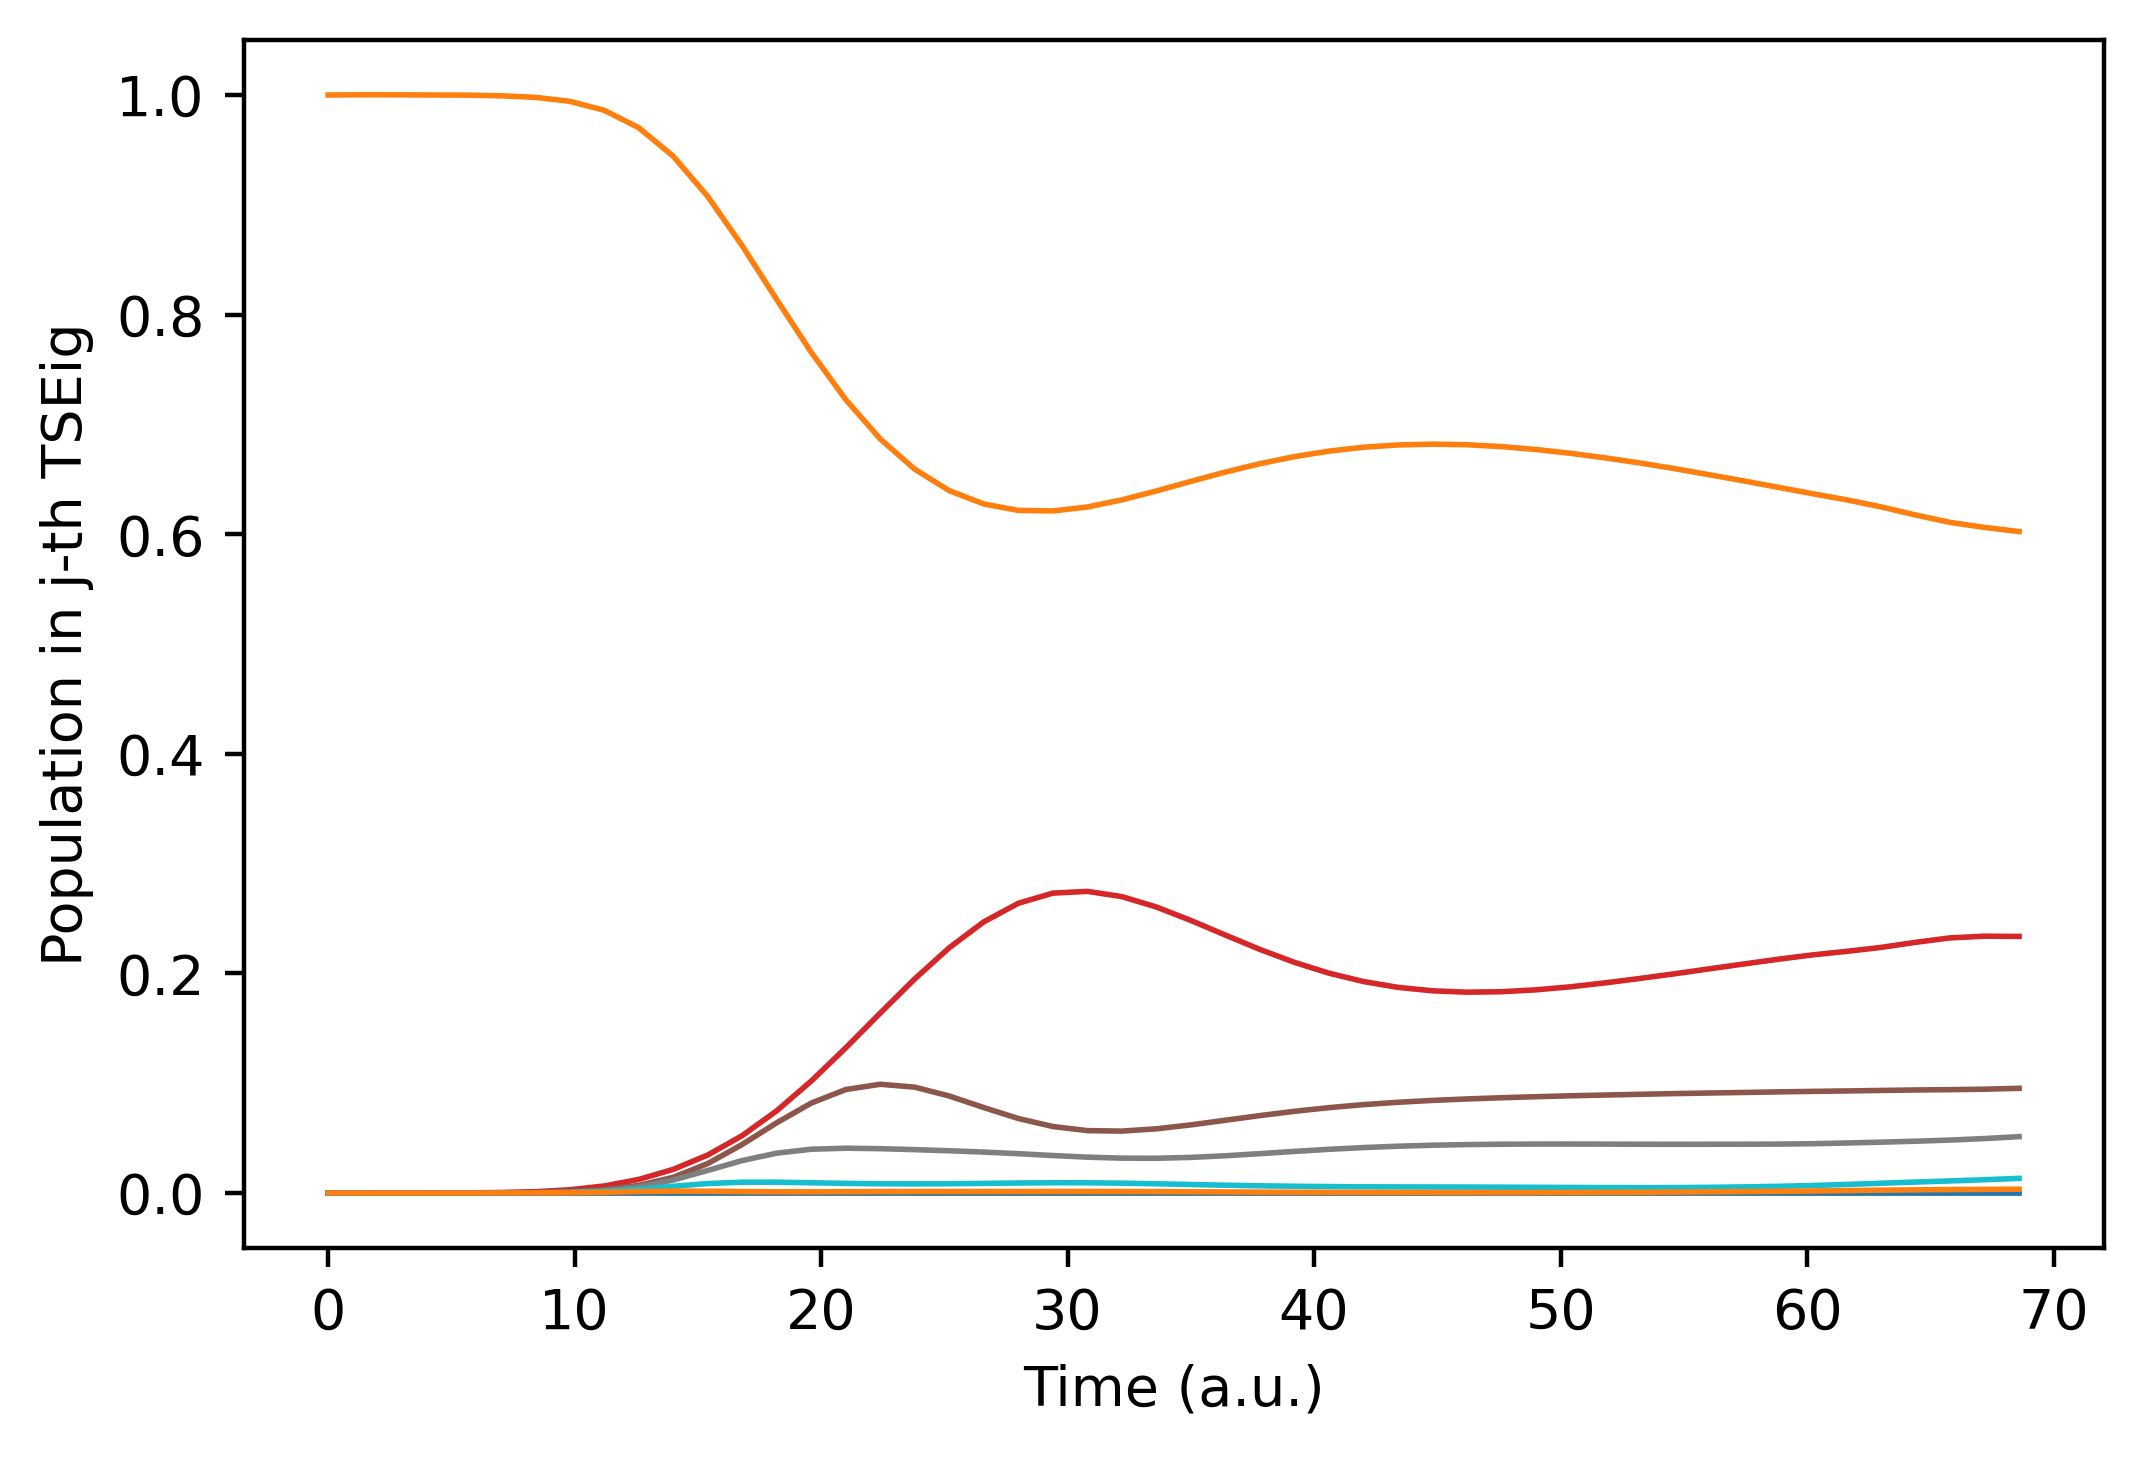
\includegraphics[width=\linewidth]{Population_GS_L5_k0_1.0.png}
    \caption{GS L=5 k=1.0}
  \end{subfigure}
  \begin{subfigure}[b]{0.36\linewidth}
    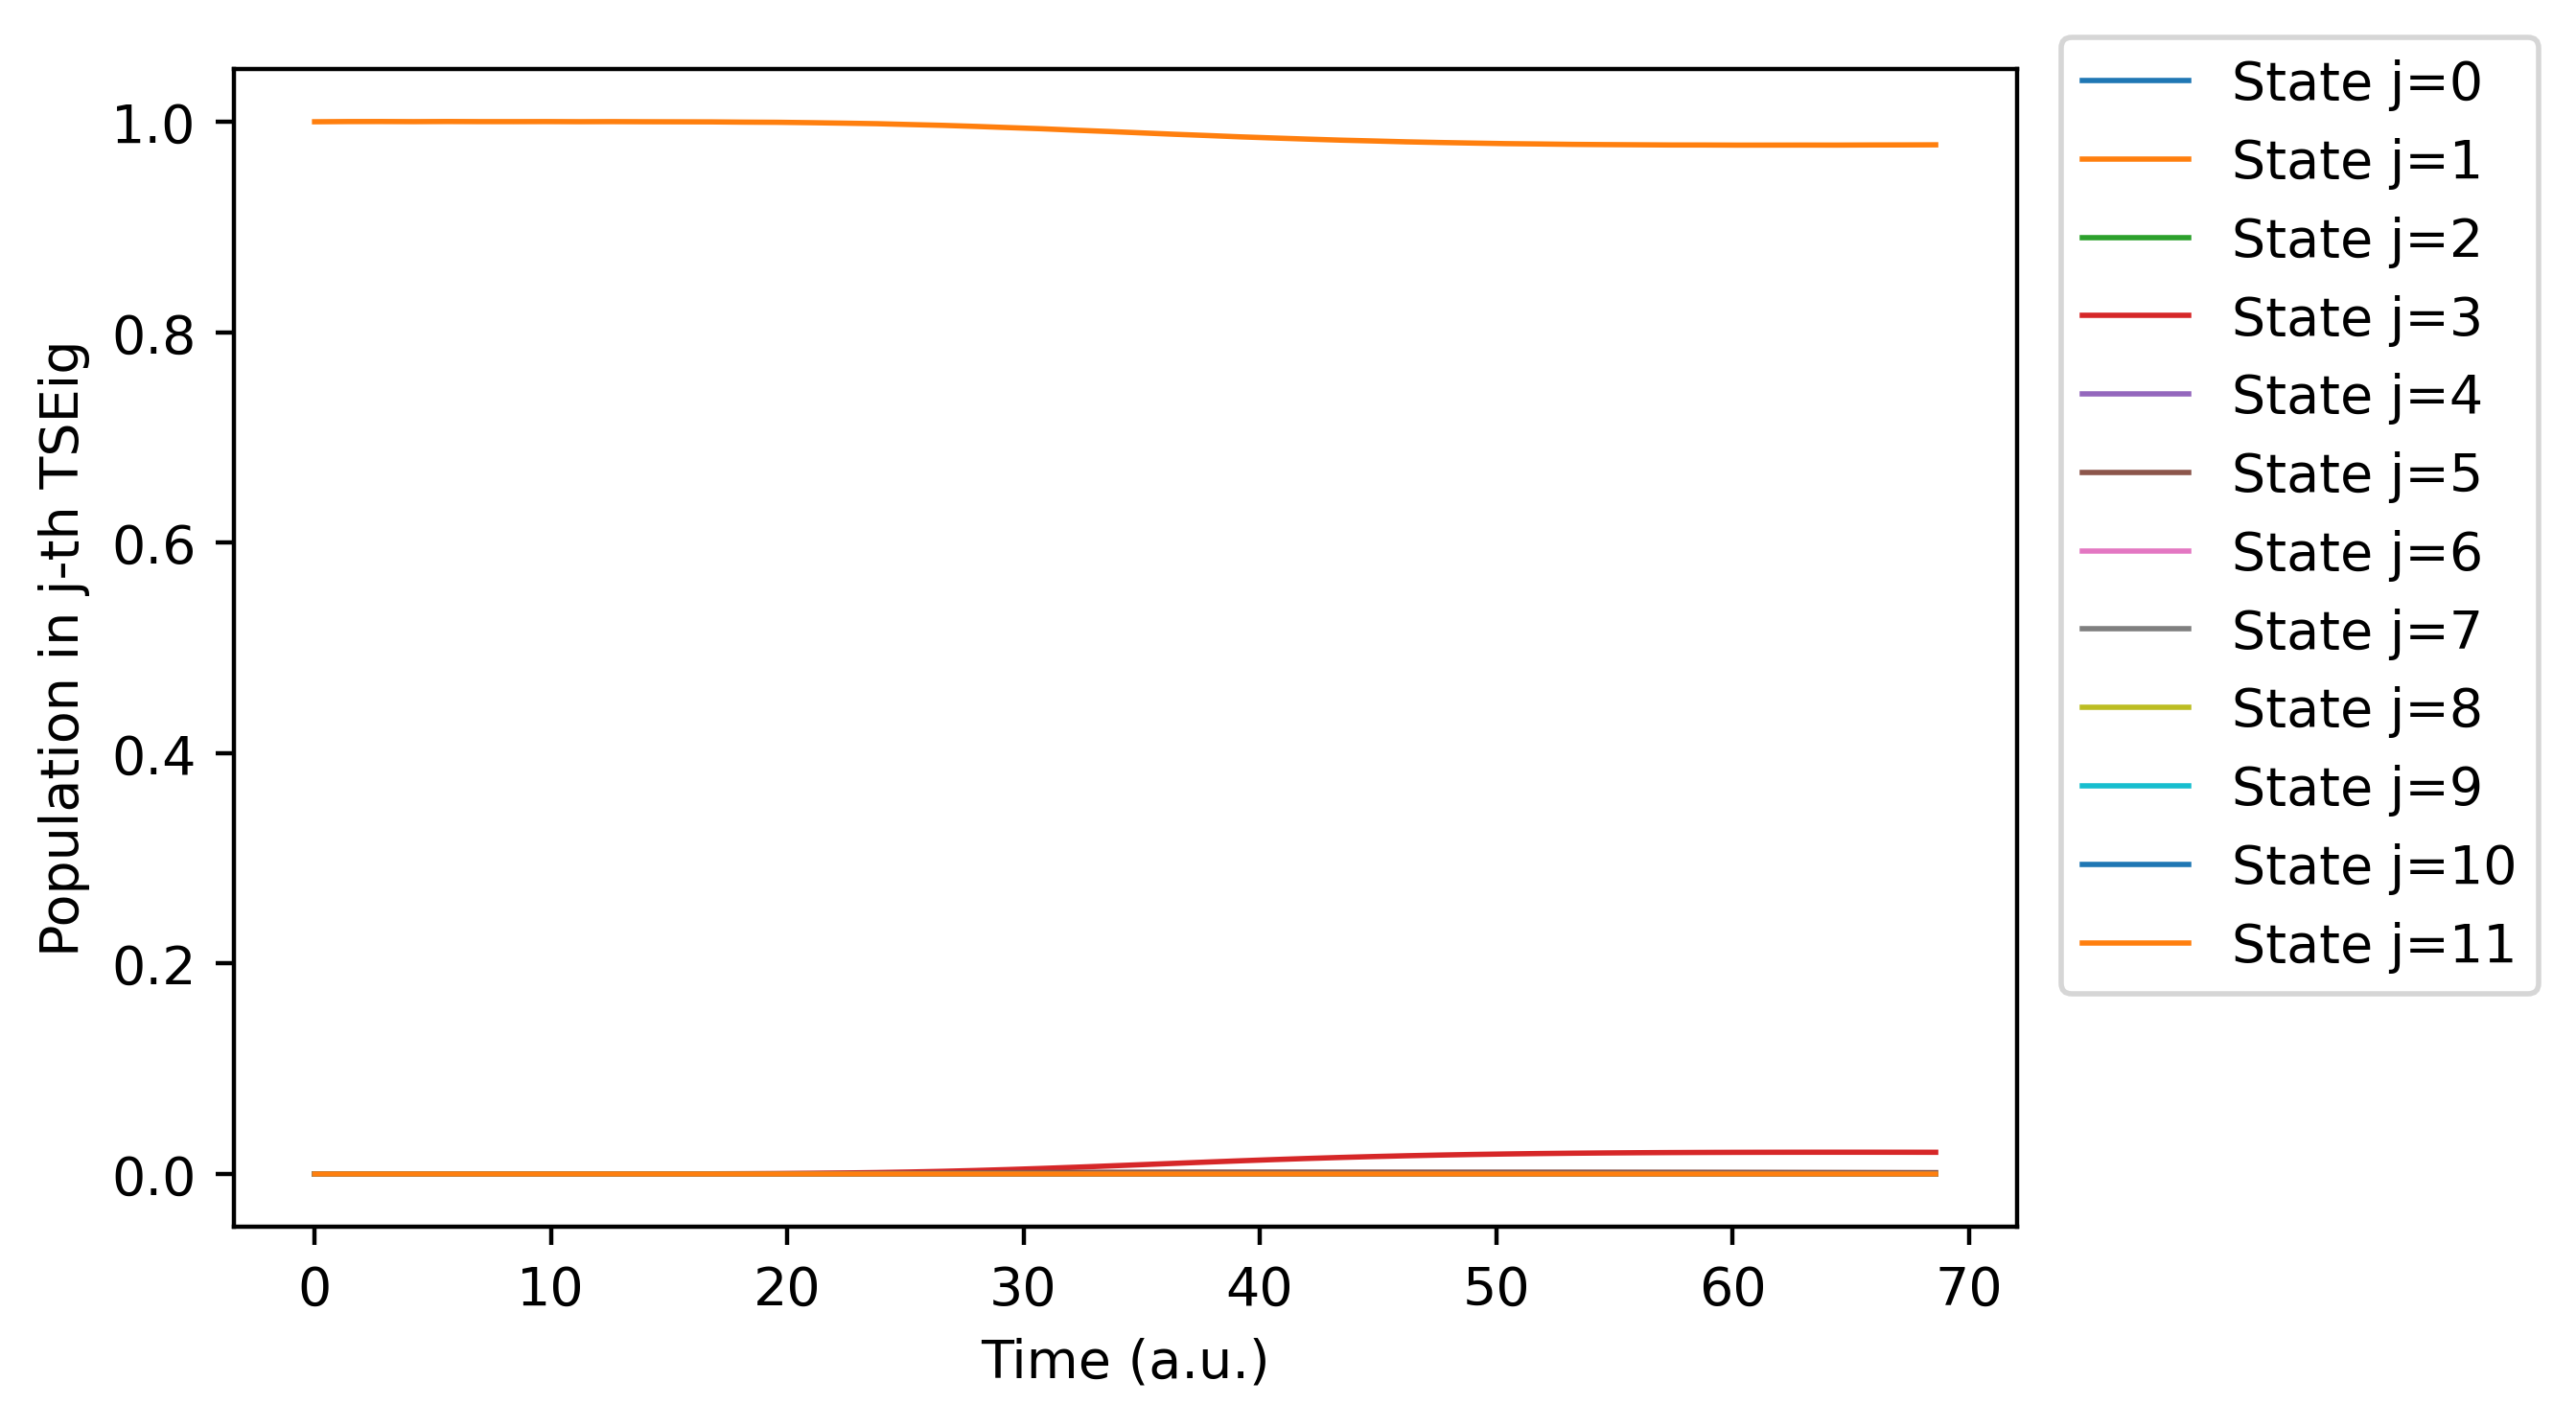
\includegraphics[width=\linewidth]{Population_GS_L8.5_k0_0.1.png}
    \caption{GS L=8.5 k=0.1}
  \end{subfigure}
    \begin{subfigure}[b]{0.30\linewidth}
    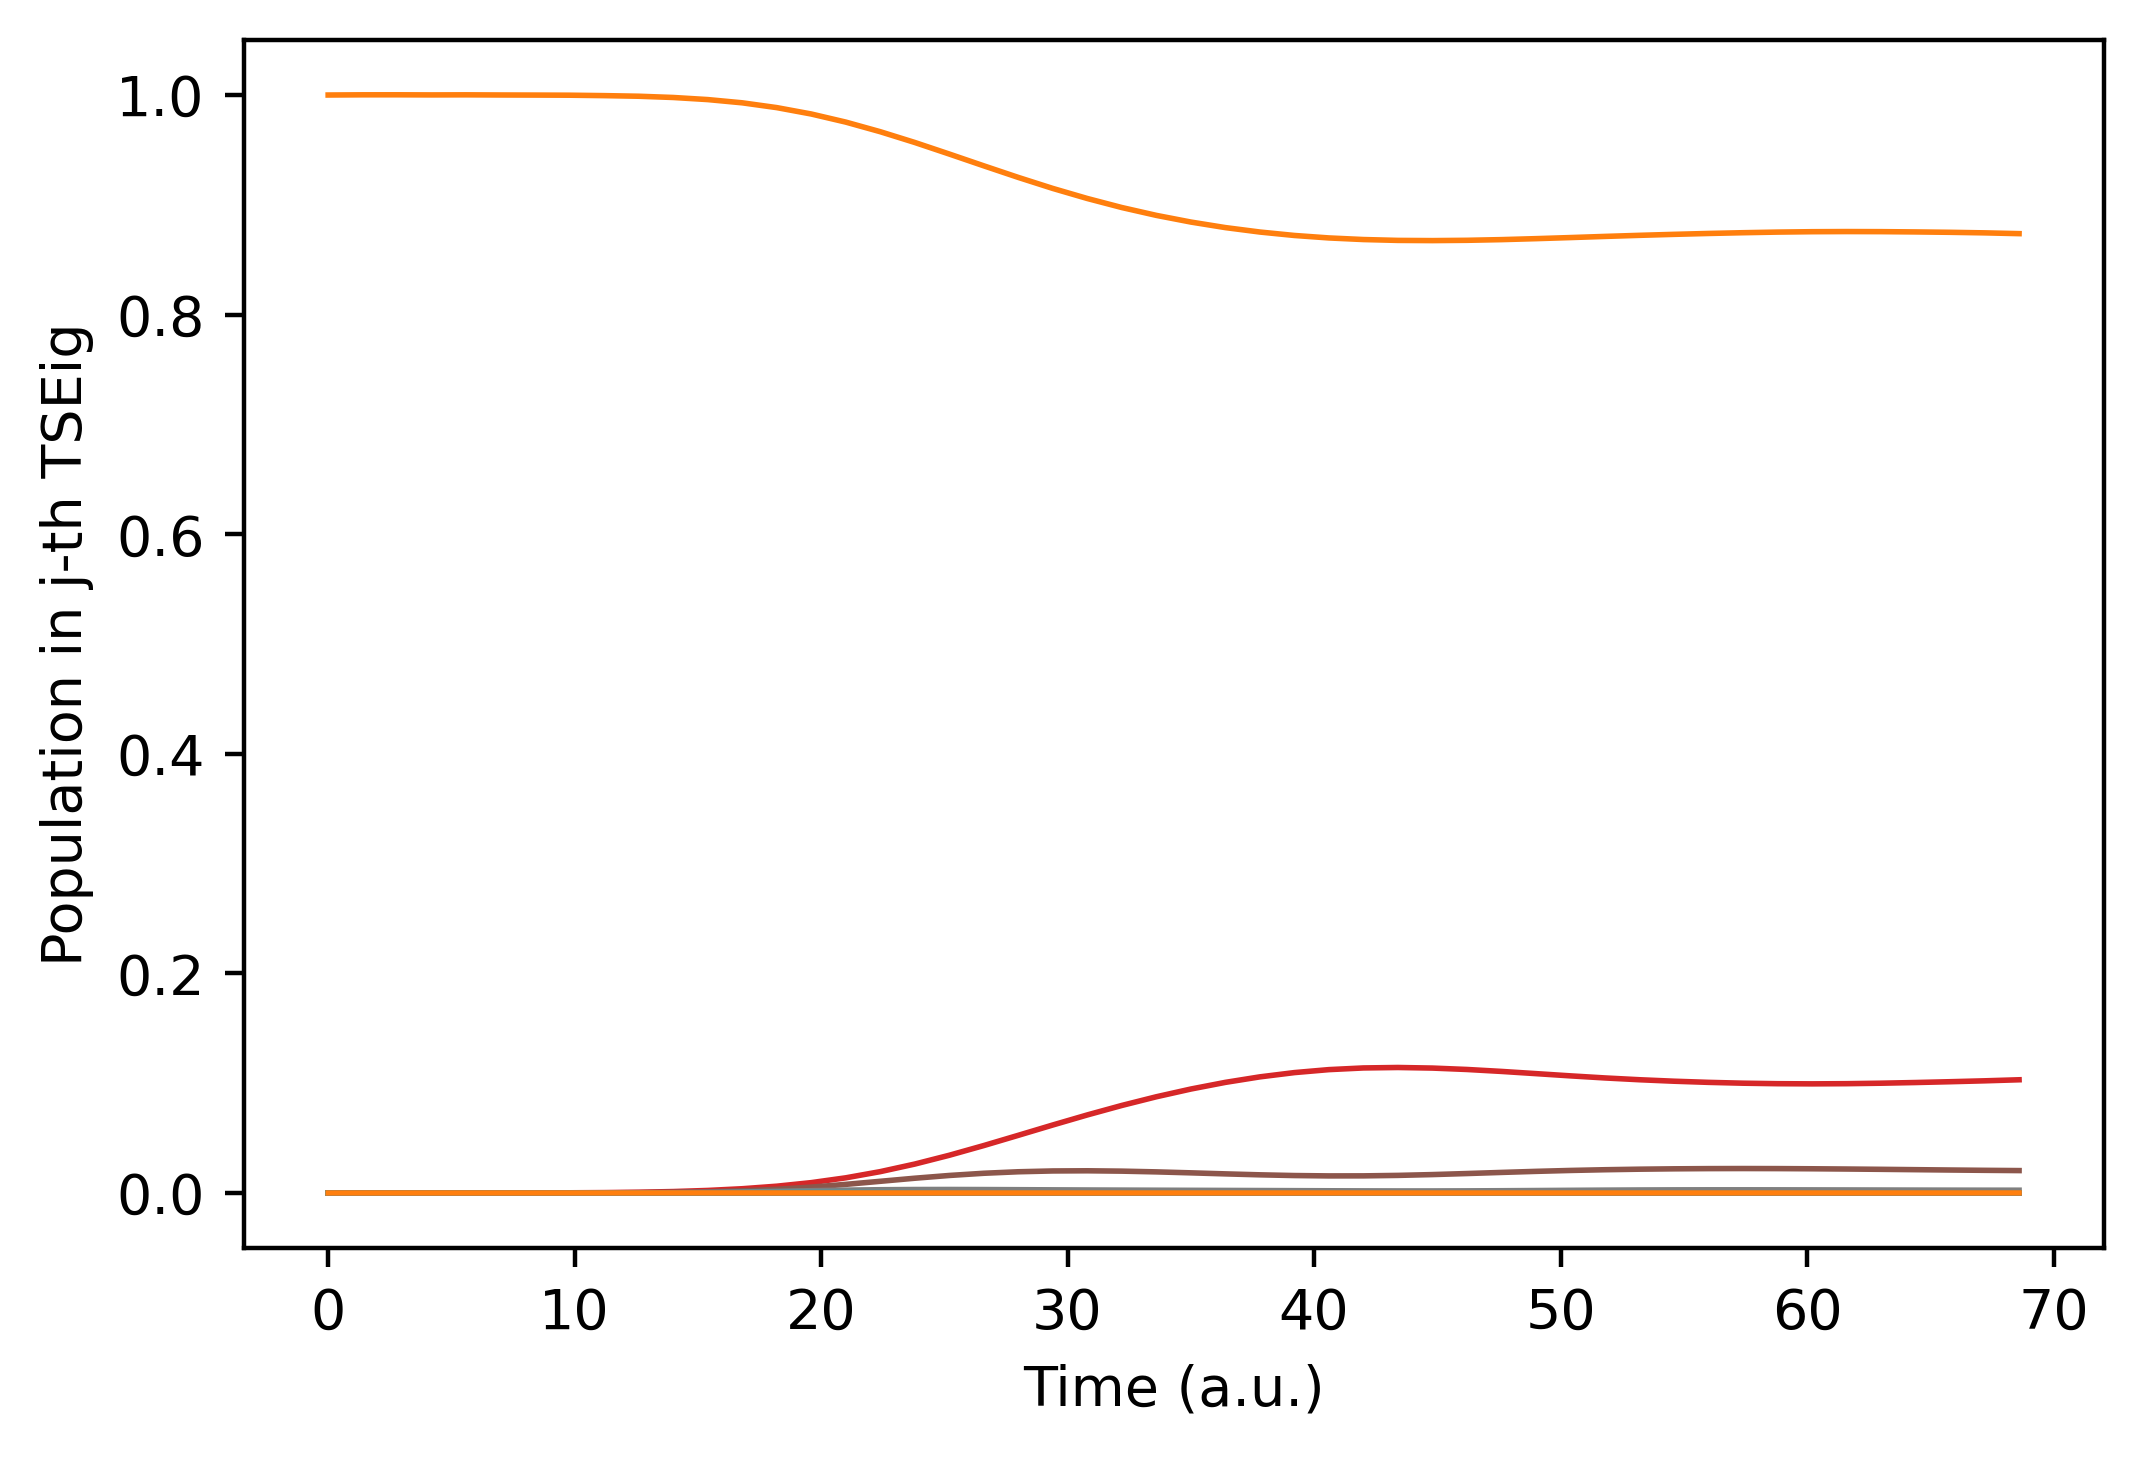
\includegraphics[width=\linewidth]{Population_GS_L8.5_k0_0.5.png}
    \caption{GS L=8.5 k=0.5}
  \end{subfigure}  
  \begin{subfigure}[b]{0.30\linewidth}
    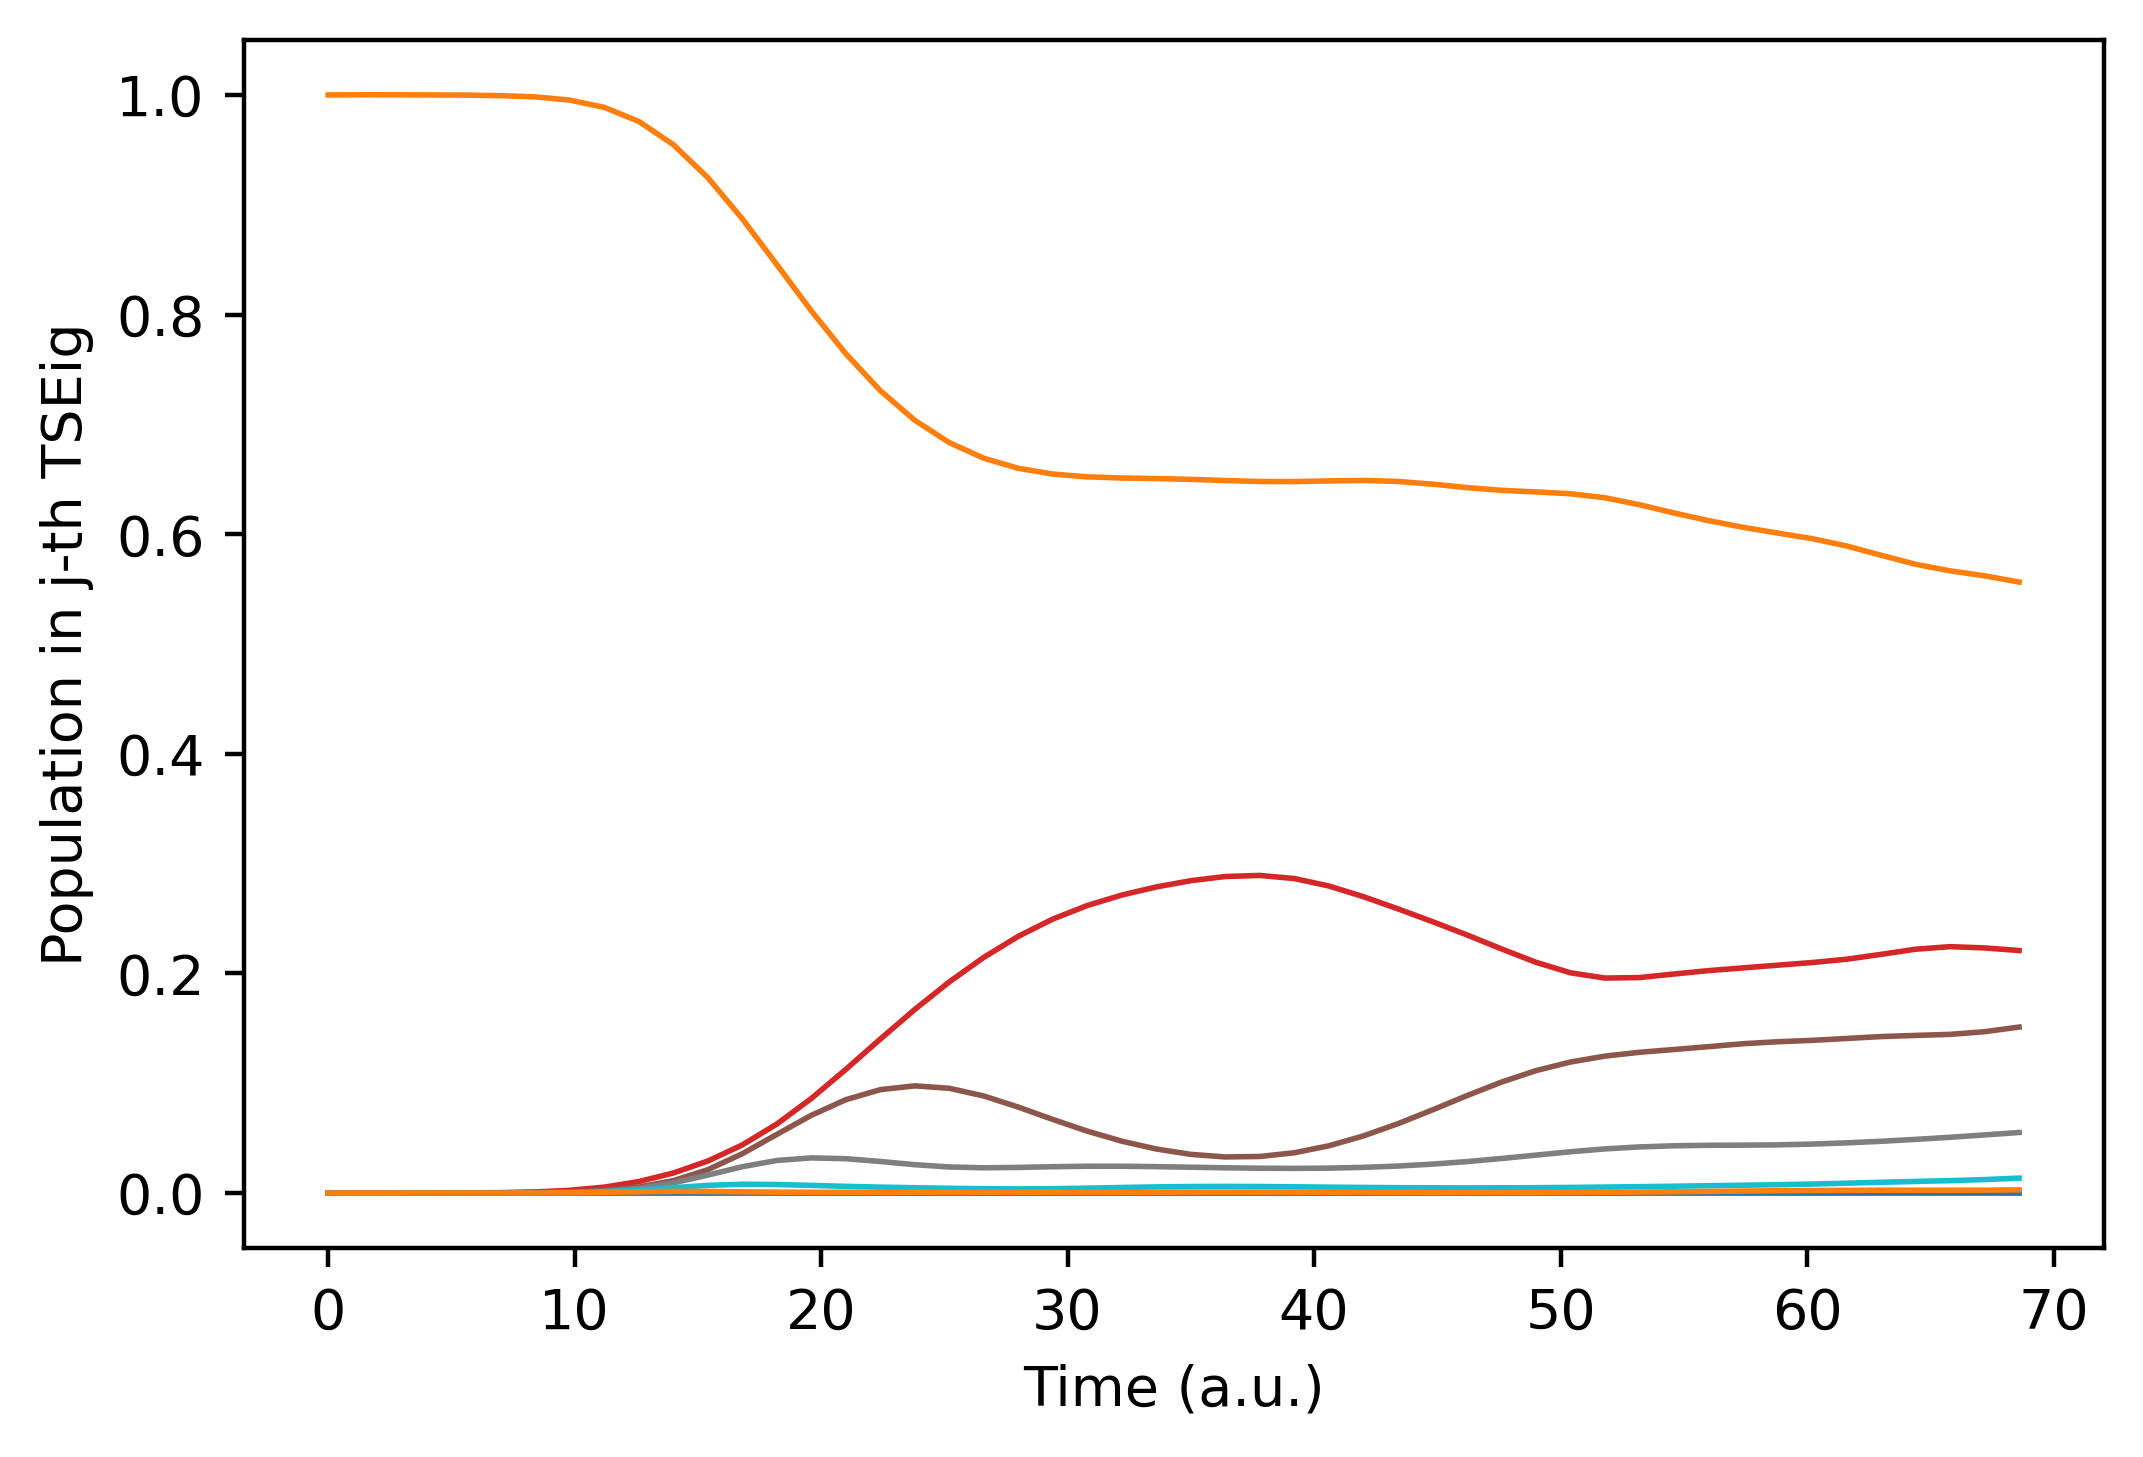
\includegraphics[width=\linewidth]{Population_GS_L8.5_k0_1.0.png}
    \caption{GS L=8.5 k=1.0}
  \end{subfigure}
  \begin{subfigure}[b]{0.36\linewidth}
    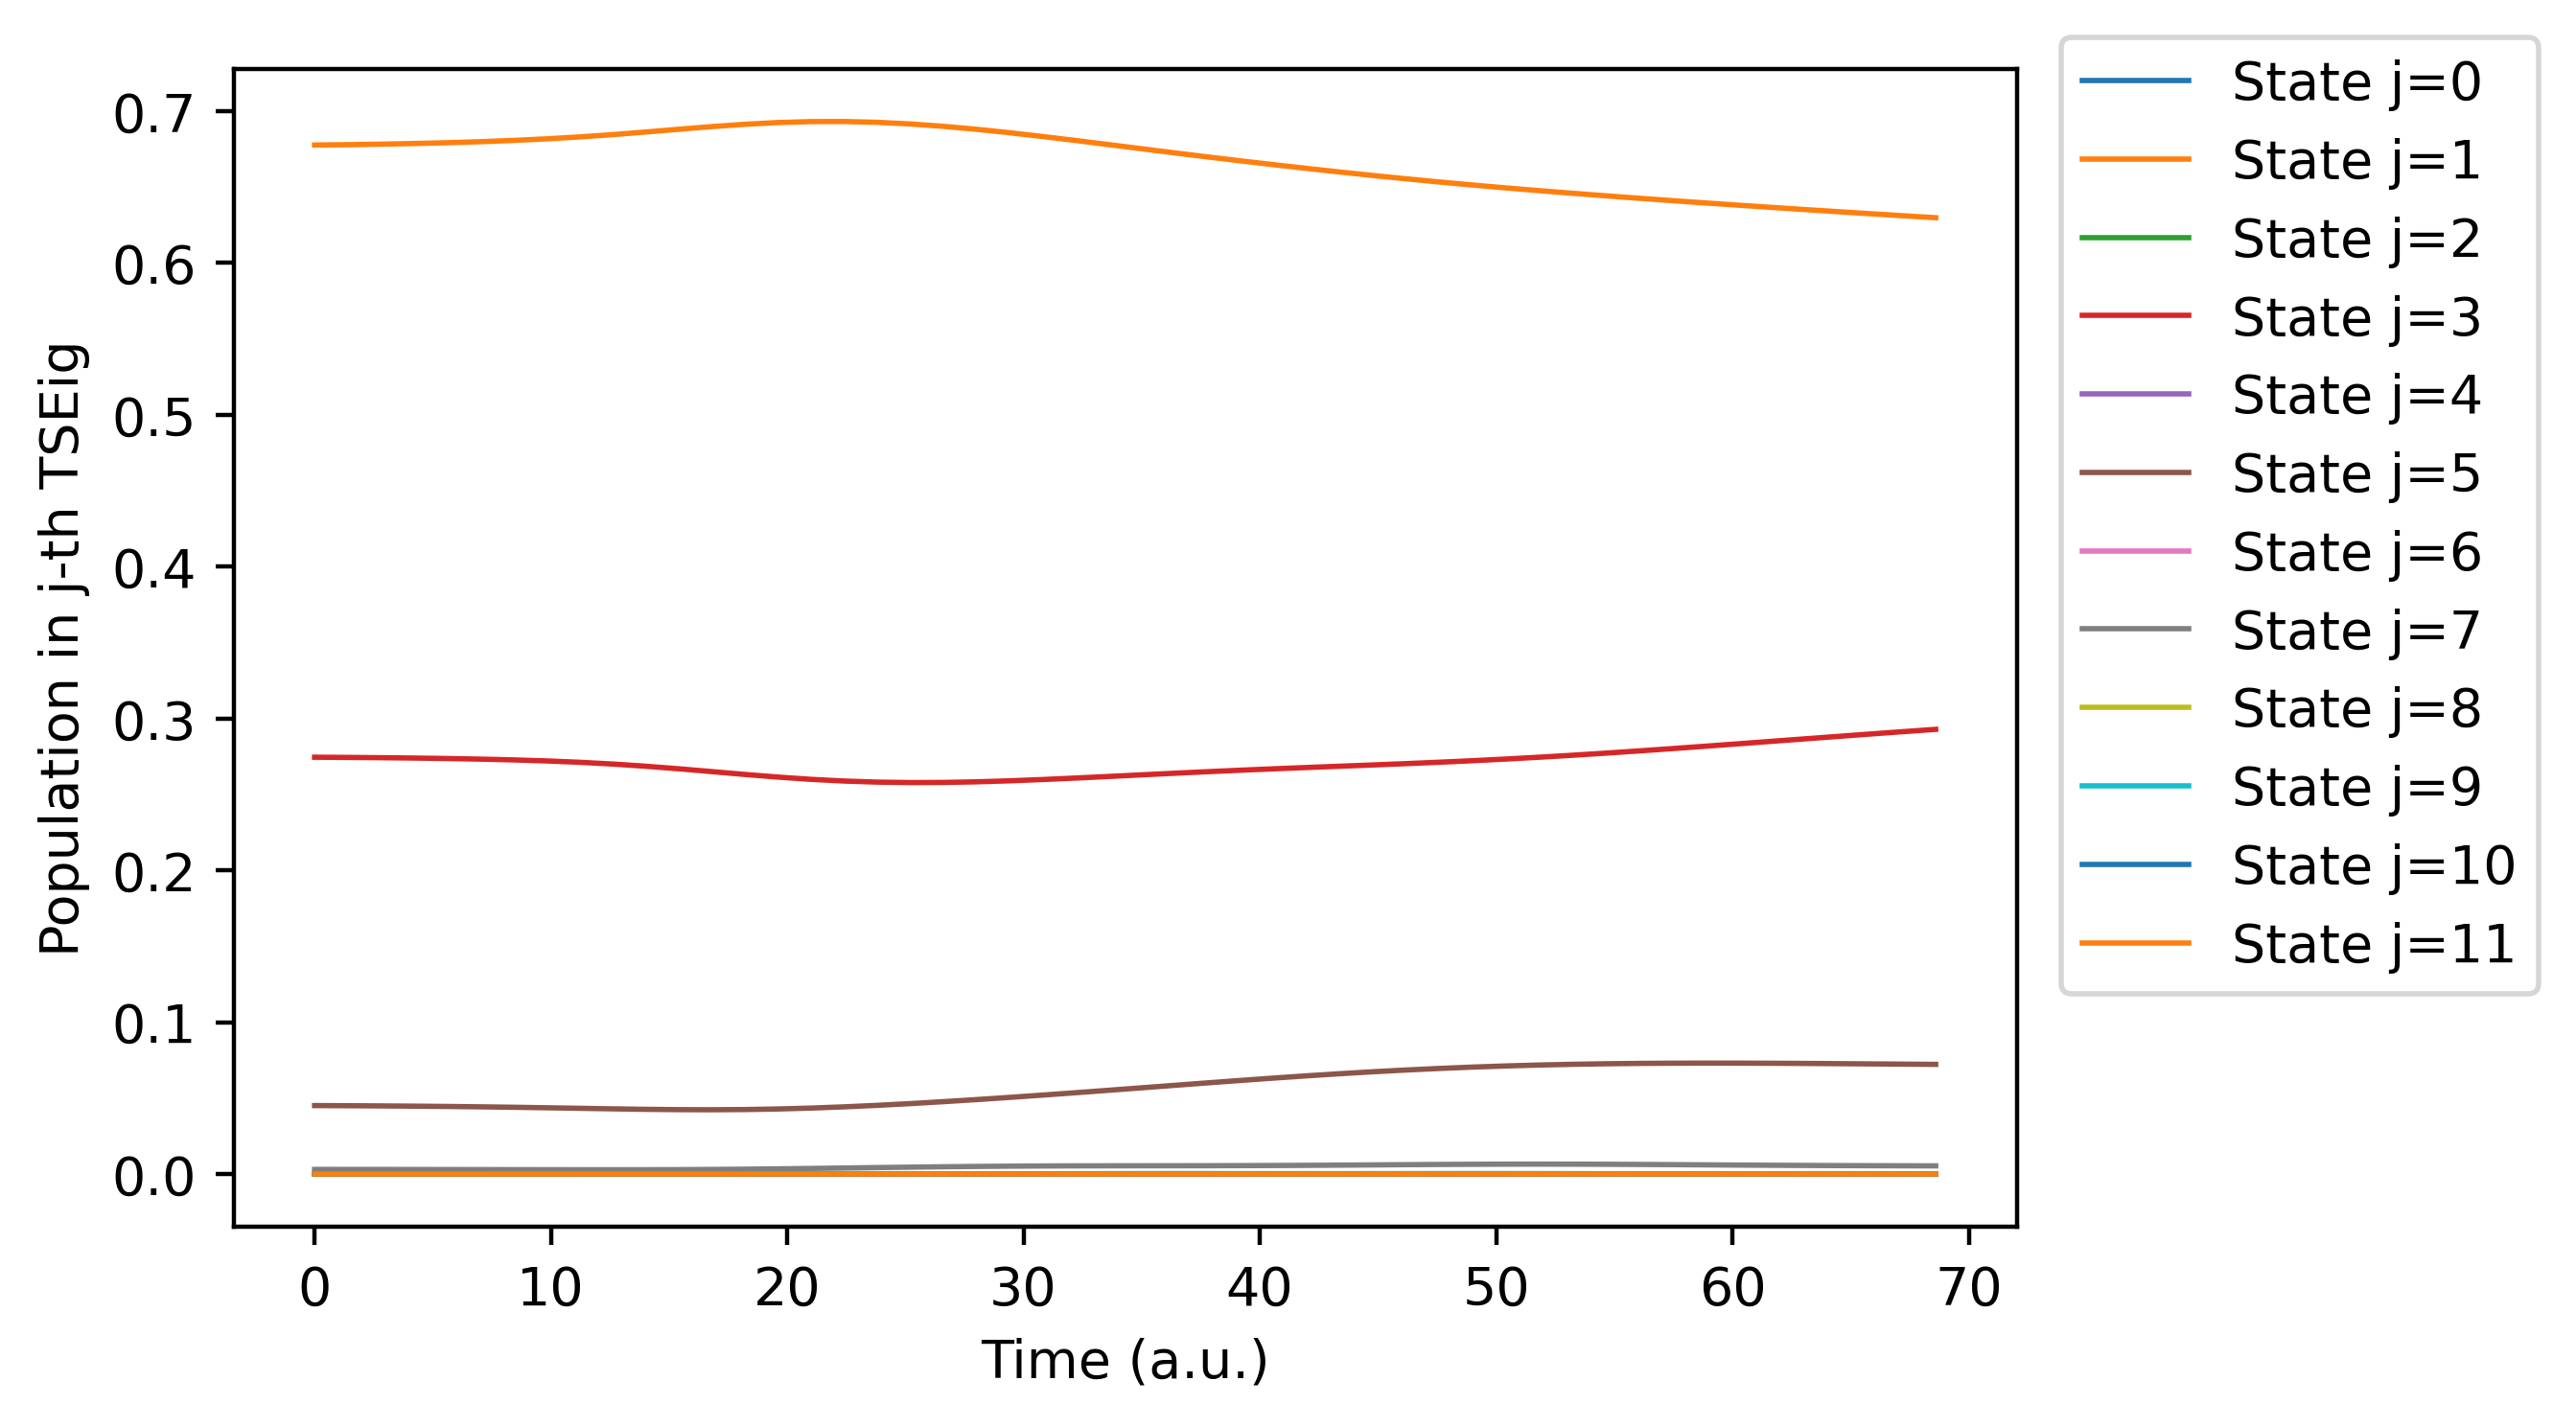
\includegraphics[width=\linewidth]{Population_GG_L5_k0_0.1.png}
    \caption{GG L=5 k=0.1}
  \end{subfigure}
    \begin{subfigure}[b]{0.30\linewidth}
    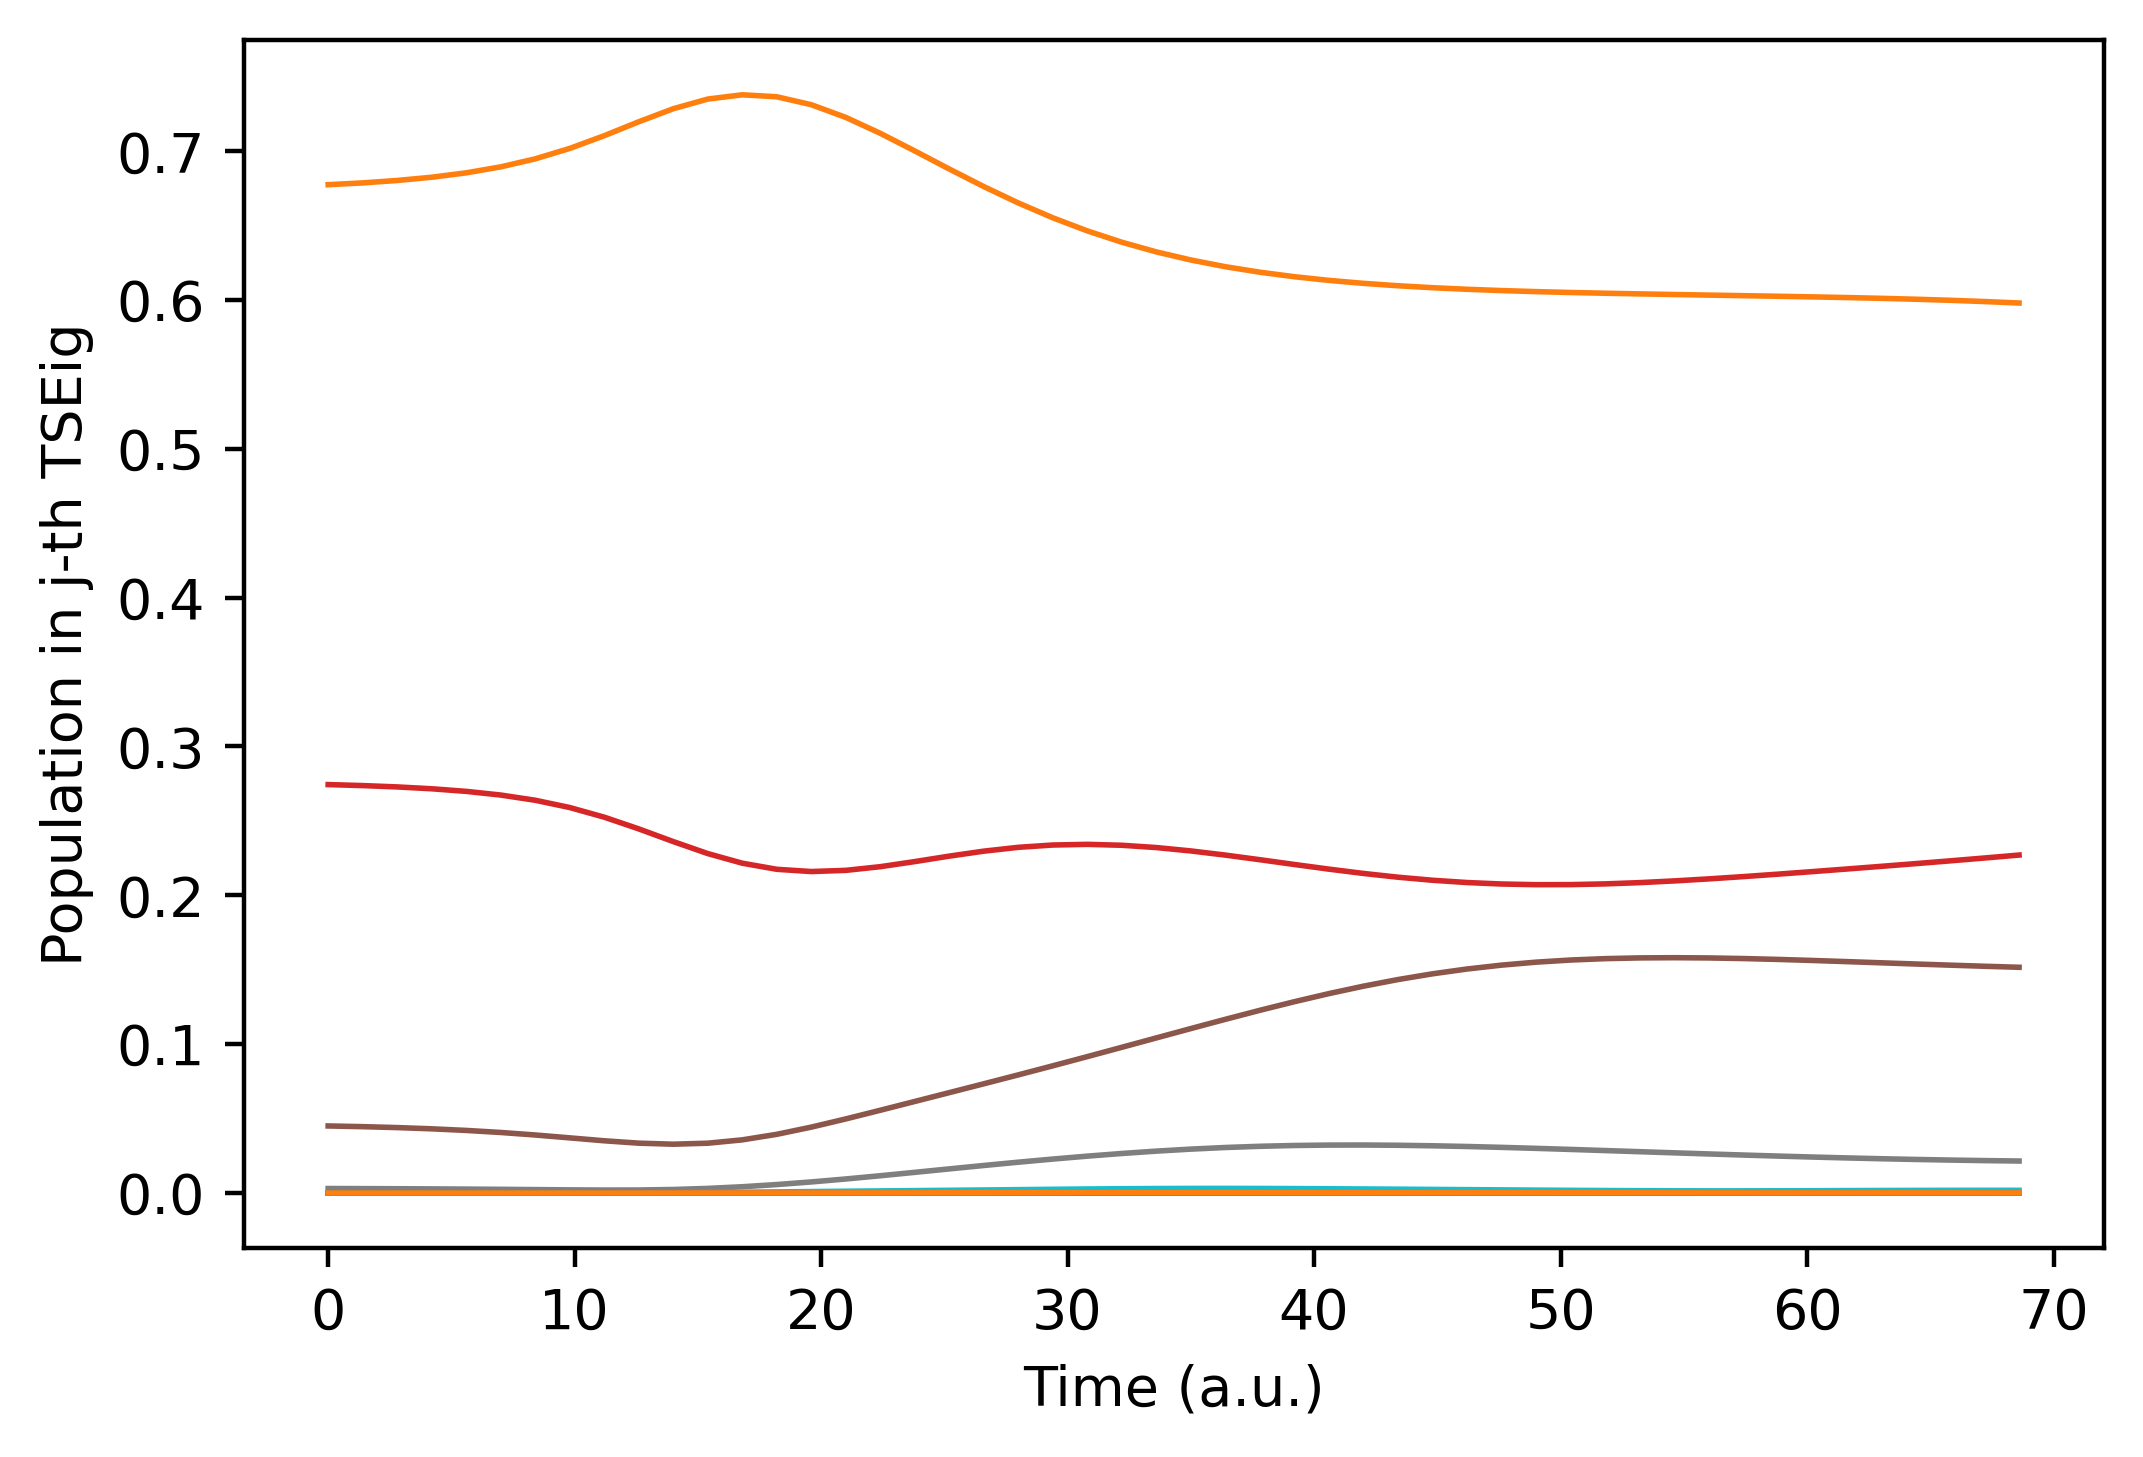
\includegraphics[width=\linewidth]{Population_GG_L5_k0_0.5.png}
    \caption{GG L=5 k=0.5}
  \end{subfigure}  
  \begin{subfigure}[b]{0.30\linewidth}
    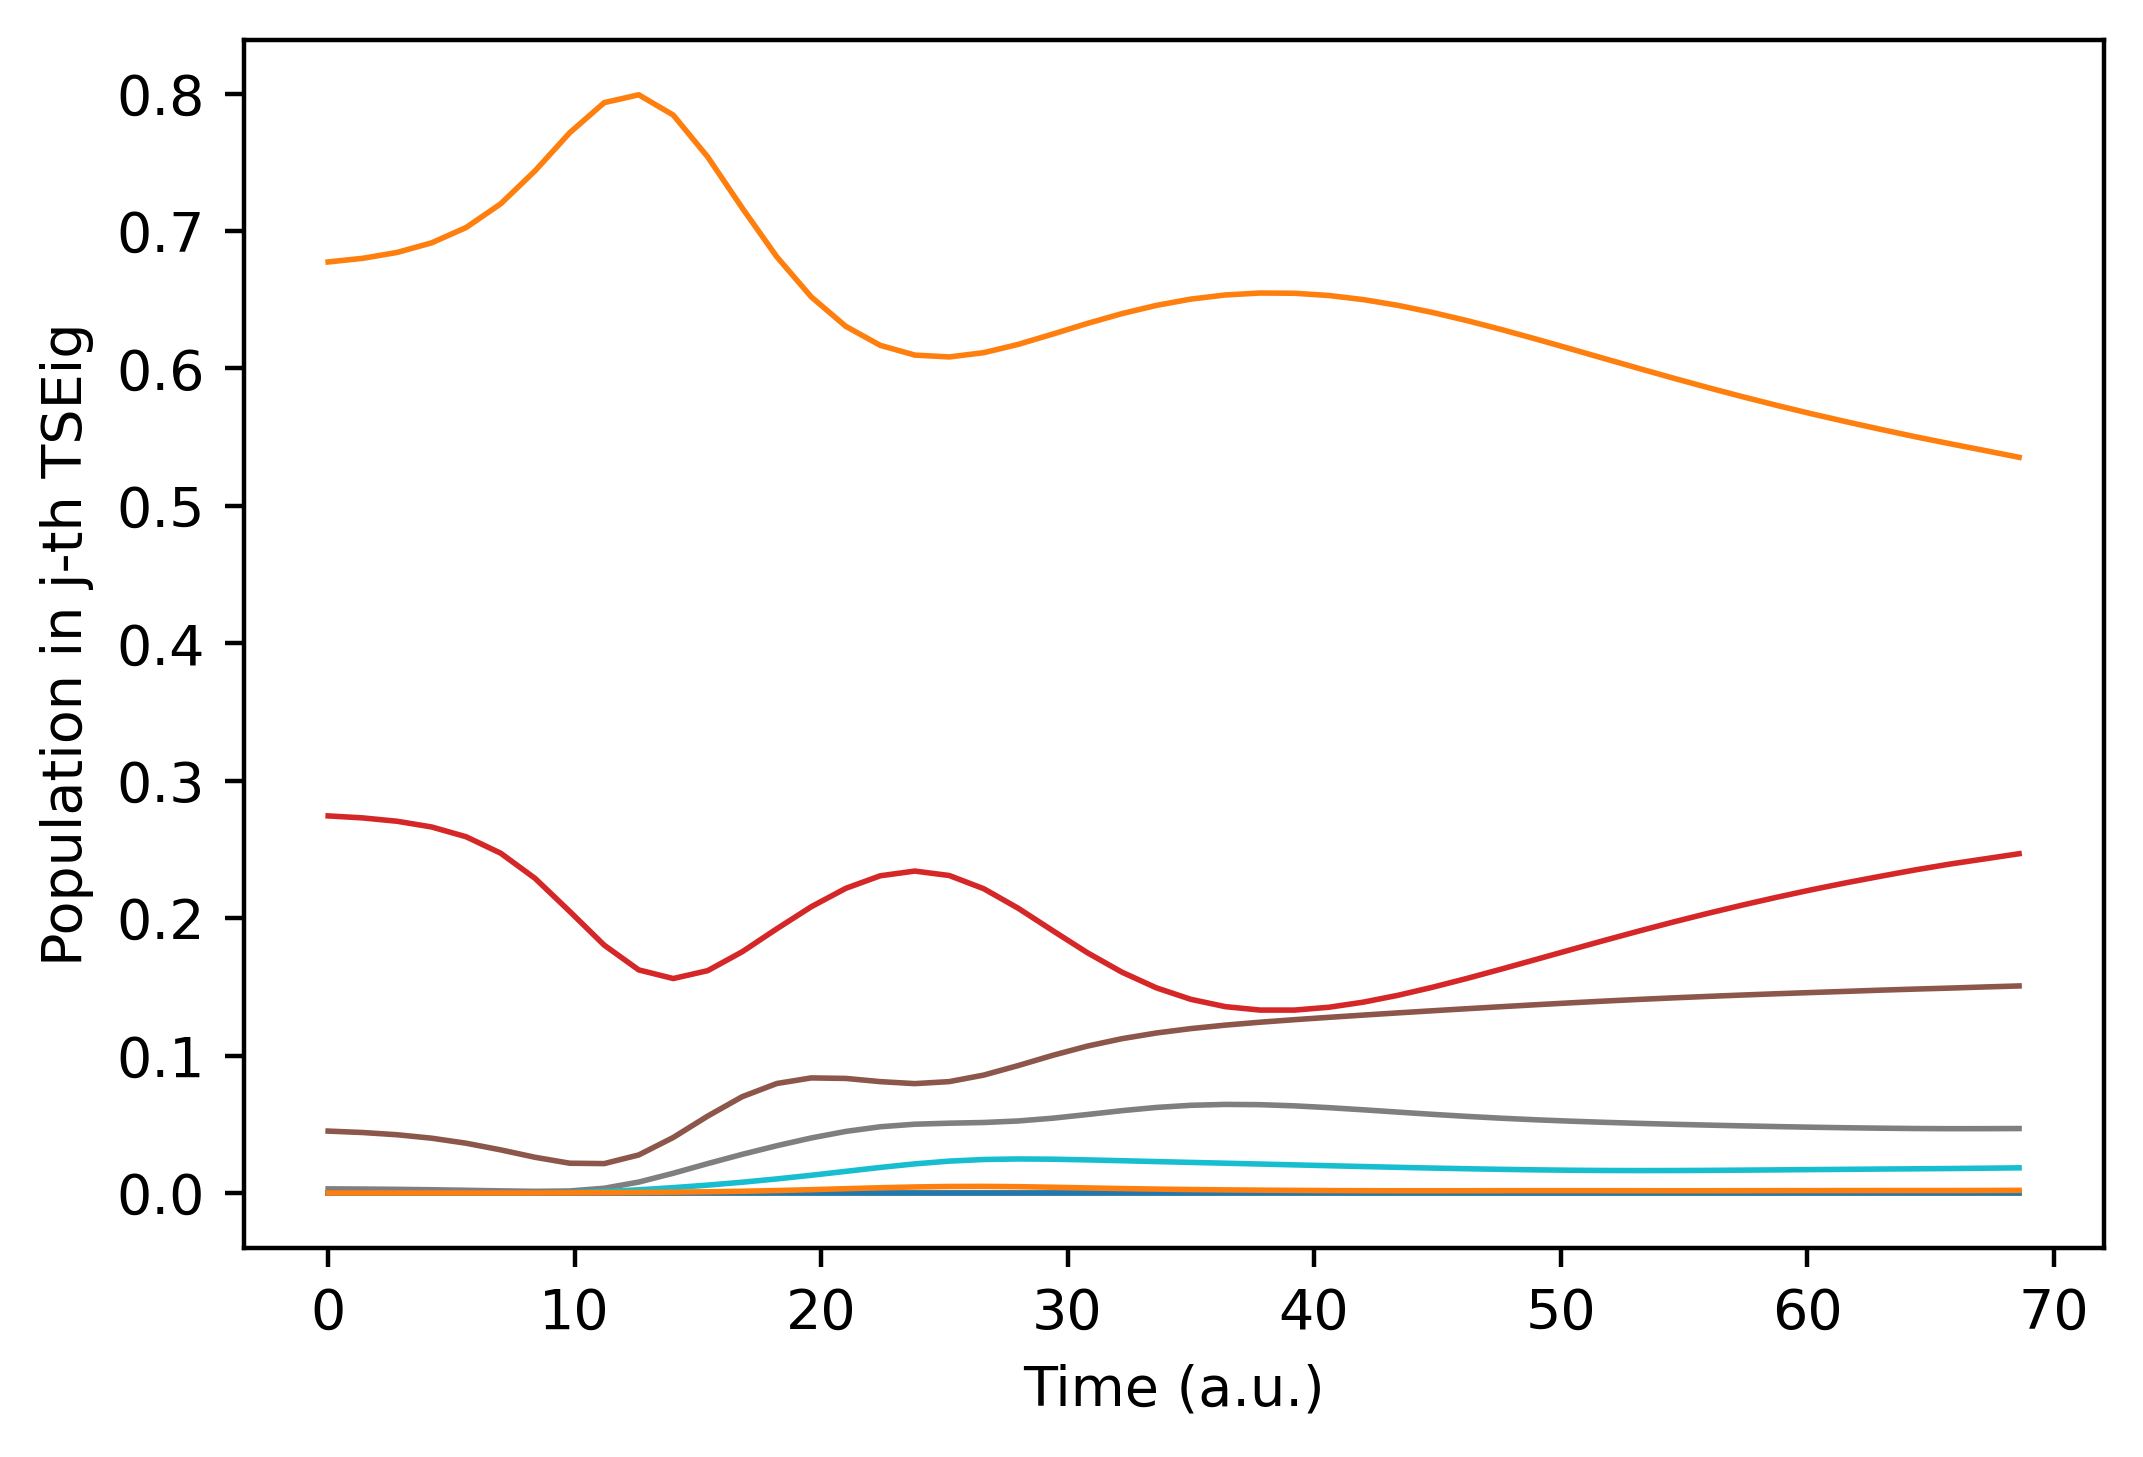
\includegraphics[width=\linewidth]{Population_GG_L5_k0_1.0.png}
    \caption{GG L=5 k=1.0}
  \end{subfigure}
  
  \begin{subfigure}[b]{0.36\linewidth}
    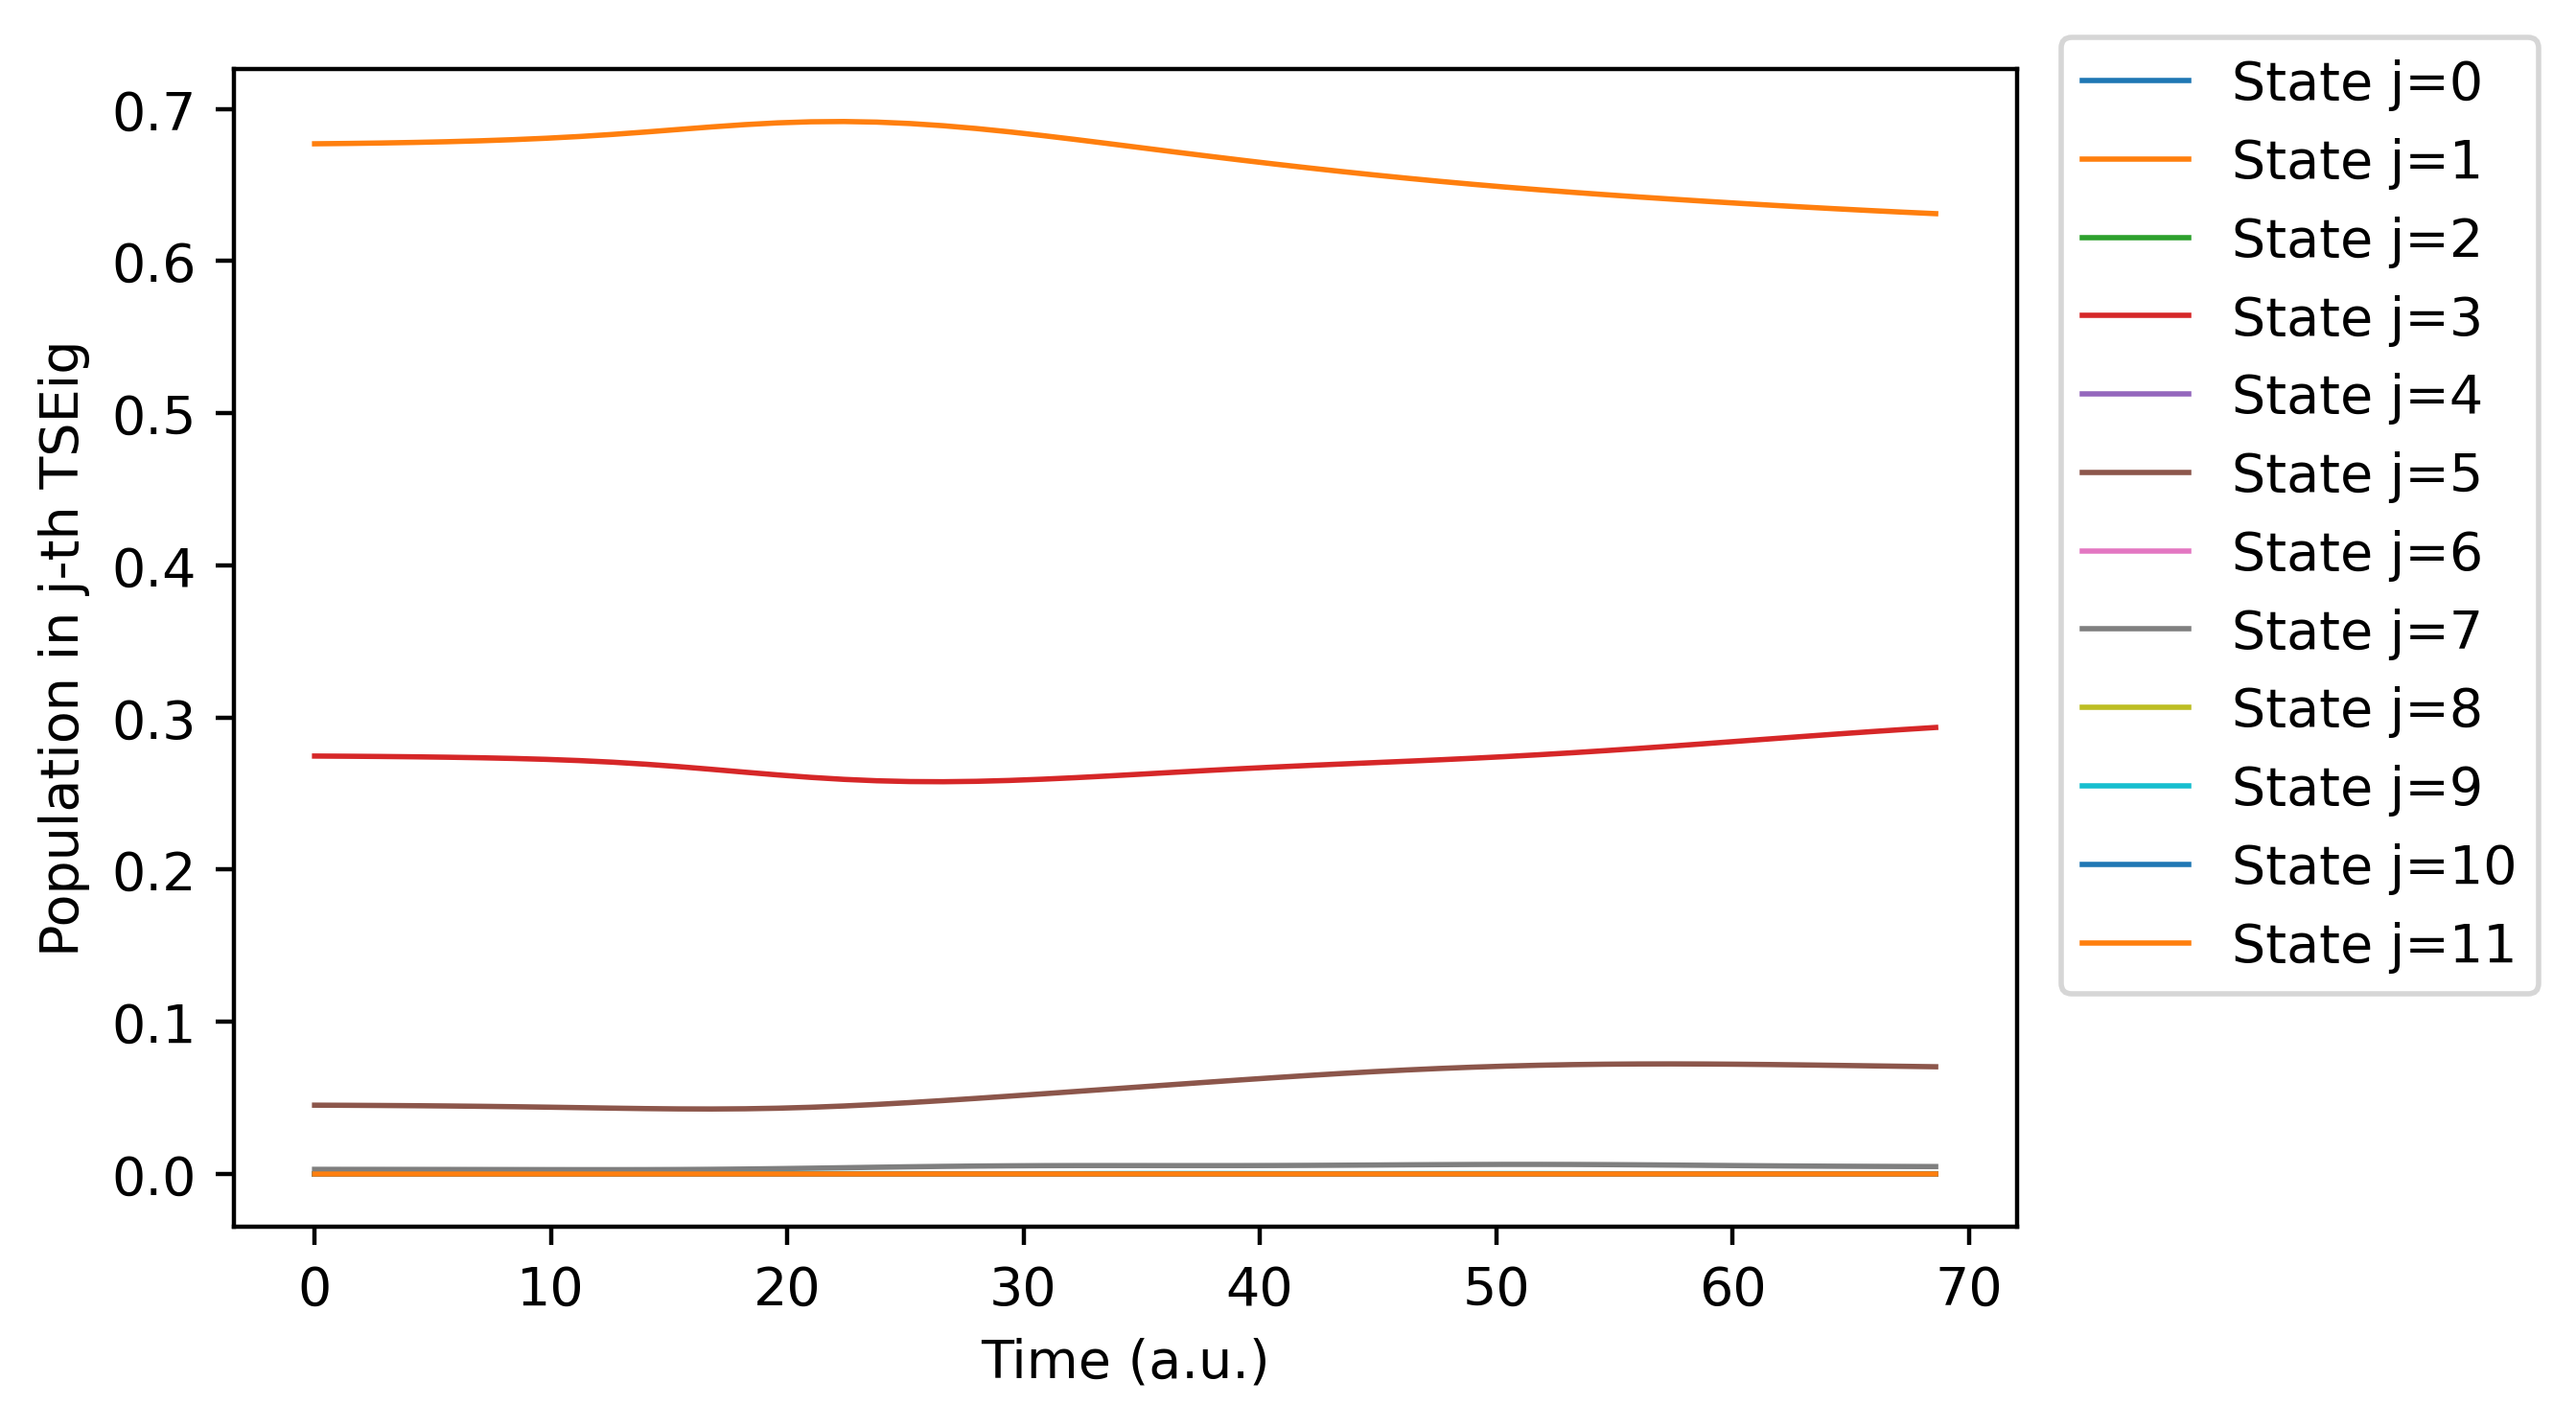
\includegraphics[width=\linewidth]{Population_GG_L8.5_k0_0.1.png}
    \caption{GG L=8.5 k=0.1}
  \end{subfigure}
    \begin{subfigure}[b]{0.30\linewidth}
    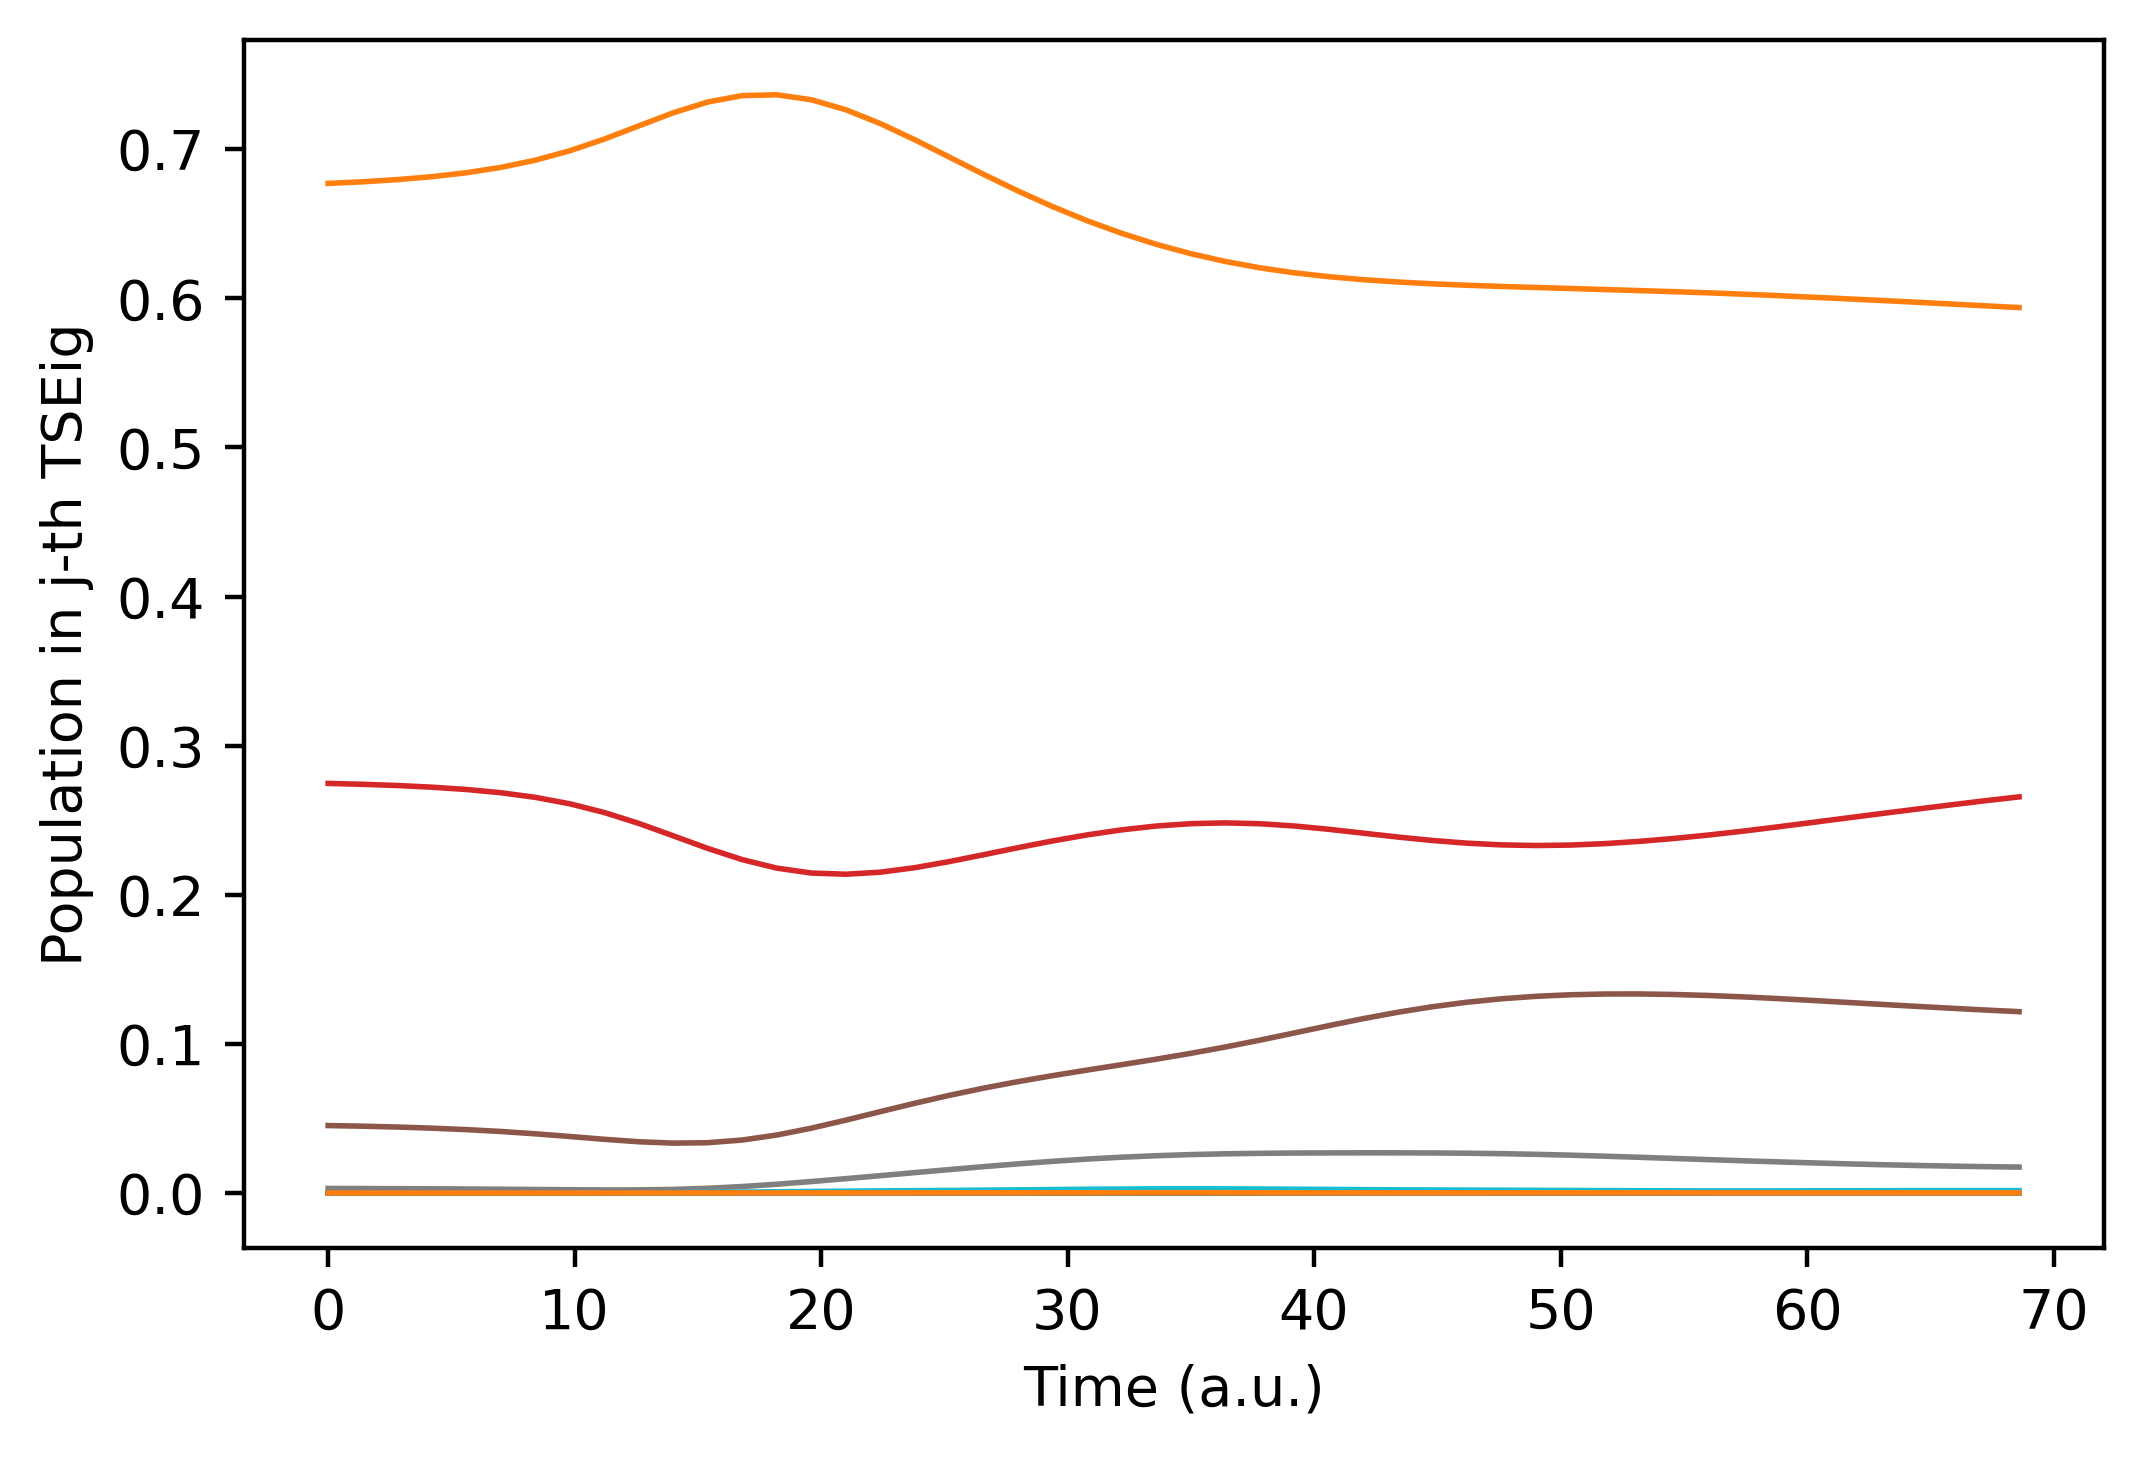
\includegraphics[width=\linewidth]{Population_GG_L8.5_k0_0.5.png}
    \caption{GG L=8.5 k=0.1}
  \end{subfigure}  
  \begin{subfigure}[b]{0.30\linewidth}
    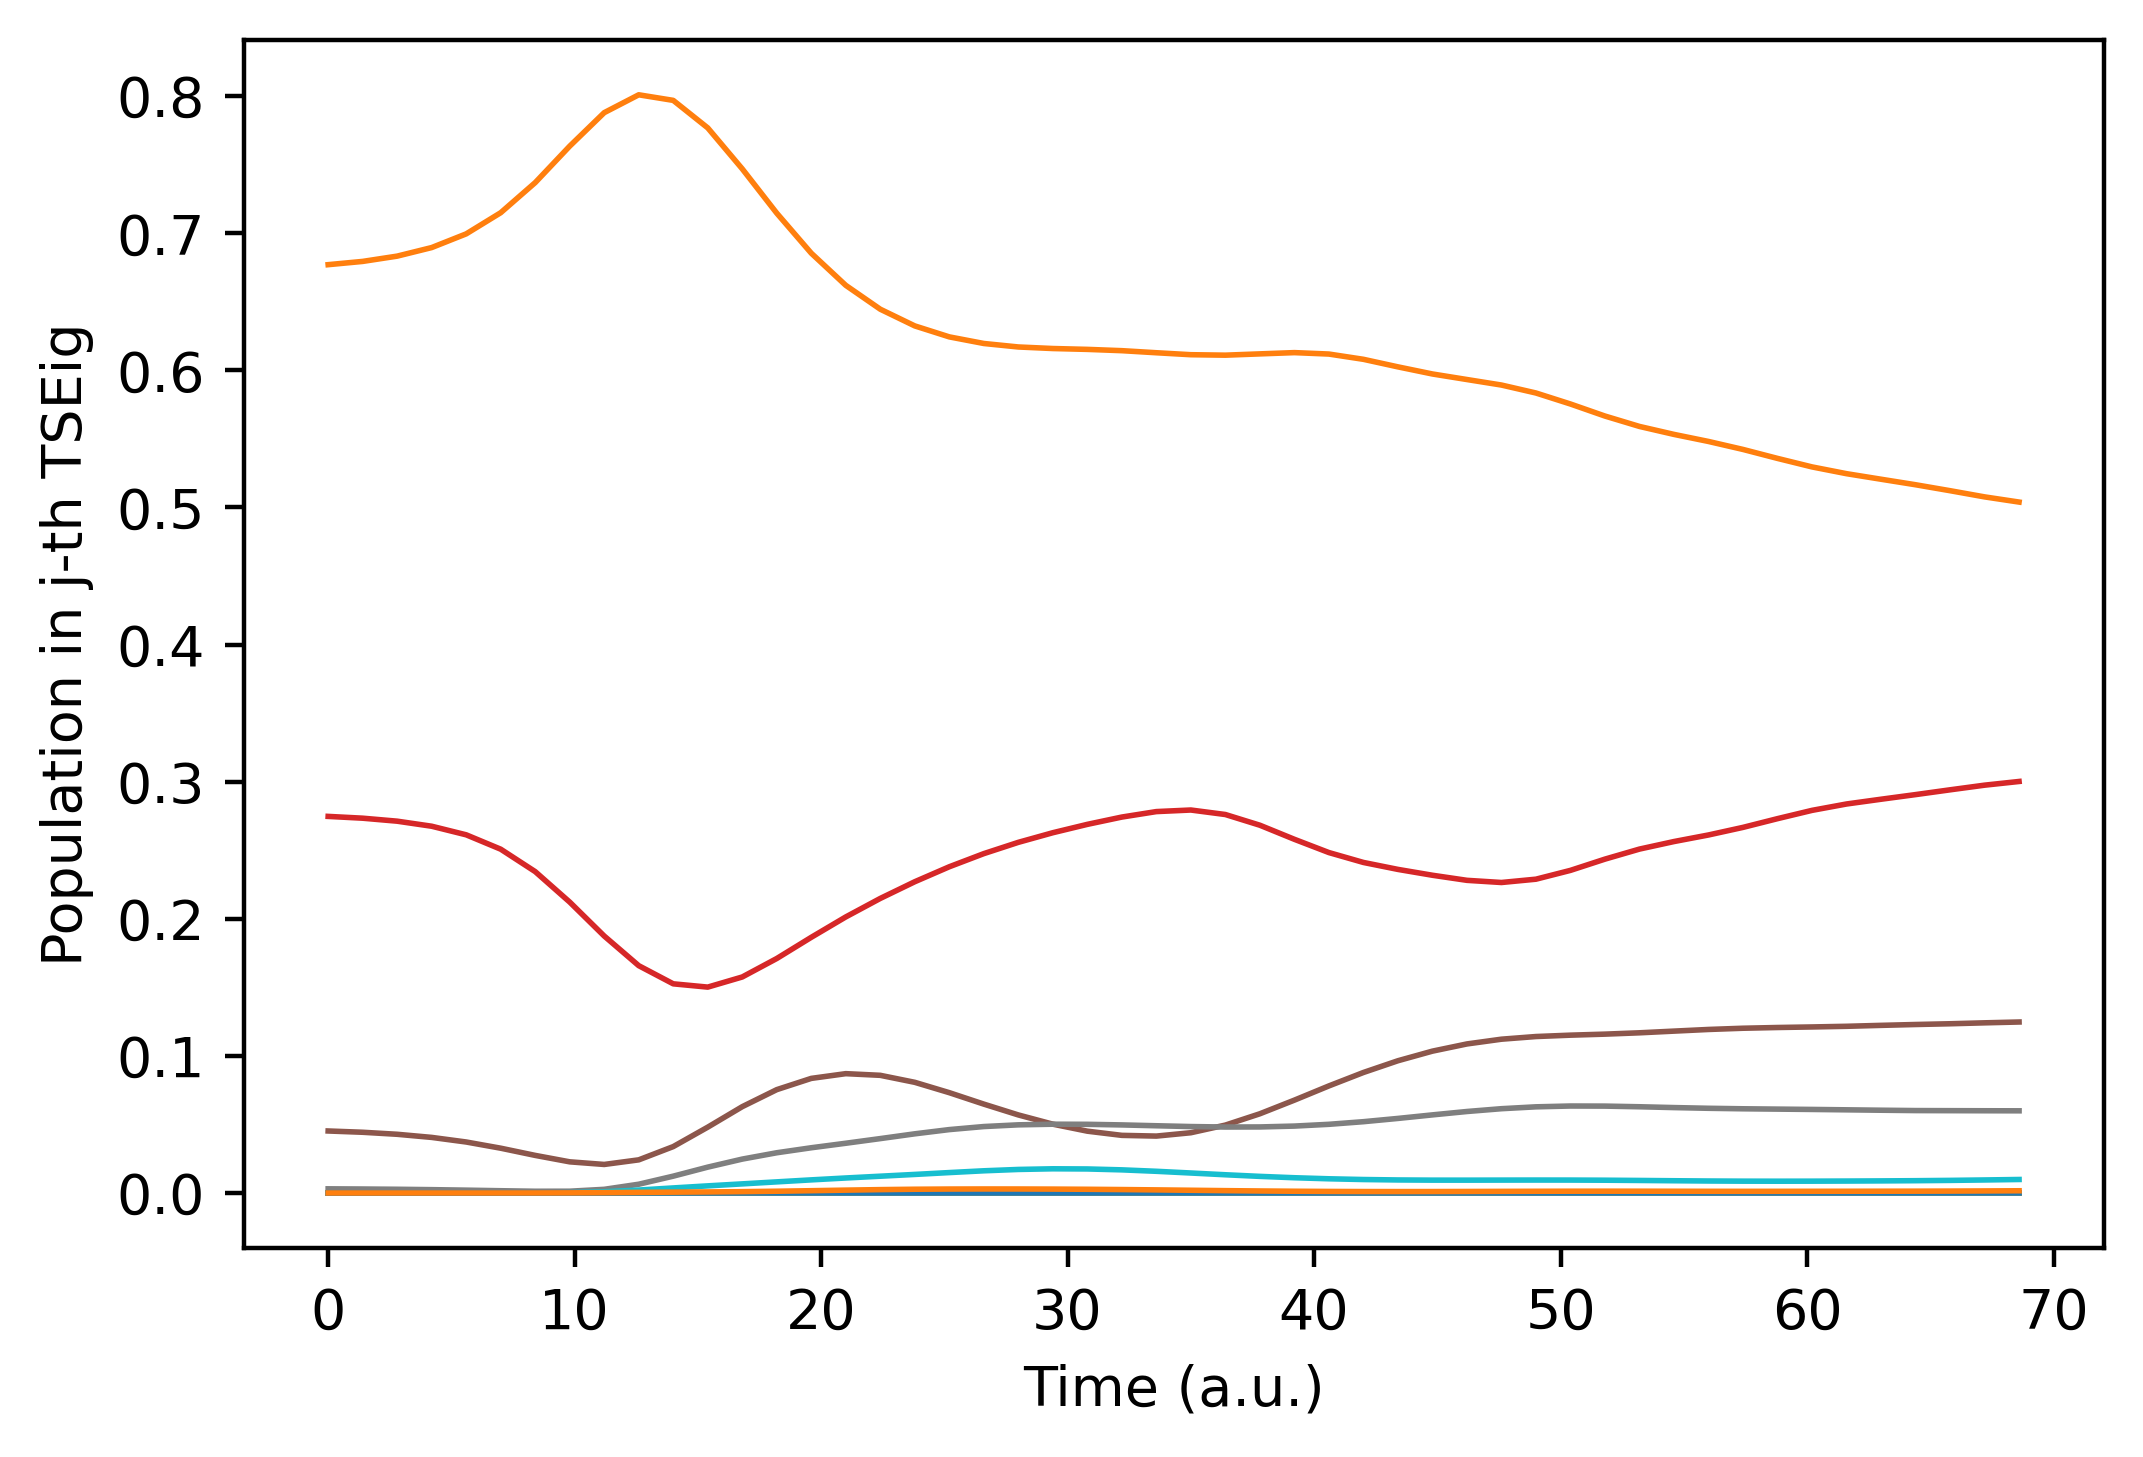
\includegraphics[width=\linewidth]{Population_GG_L8.5_k0_1.0.png}
    \caption{GG L=8.5 k=0.1}
  \end{subfigure}
  
  \caption{ Population of the $j-th$ adiabatic state as a function of time $P_j(t)=\int_{-\infty}^\infty |\chi^j_x(x,t)|^2dx $. Note $GS:=Gauss(x;\mu_x, \sigma_x, k_x)\Phi^1_x(y)$, and $GG:=Gauss(x;\mu_x, \sigma_x, k_x)Gauss(x;\mu_y, \sigma_y, k_y)$. Computed using the full wavefunction got with the CN method. Note that there is only population in odd states due to the symmetry of the problem.}
  \label{fig:popsInTime}
\end{figure}
\newpage

For these two settings of slit width, we then applied the two approximating algorithms suggested so far: the Hermitian approach and the truncated Born-Huang expansion (for several different $J$) in both settings of slit width. 

An ensemble of $M$ Bohmian trajectories sampled according to the full wavefunction's probability density, should replicate the probability density of the full wave-function. Thus, we can assert the methods by comparing the transmission of the full wave-function through the narrowest part of the channel integrated using CN, and the proportion of Bohmian trajectories transmitted using each of the approximate algorithms. In Figures \ref{fig:transm_GS_L5} and \ref{fig:transm_GS_L85} one can find the transmission study as a function of the initial momenta range described earlier for the initial wavepacket GS and narrowness $L_{min}=5$ and $8.5$, respectively. We see the same but for the wave-packet GG in Figures \ref{fig:transm_GG_L5} and \ref{fig:transm_GG_L85}.



\begin{figure}[p]
  \centering
  \begin{subfigure}[b]{1.1\linewidth}
    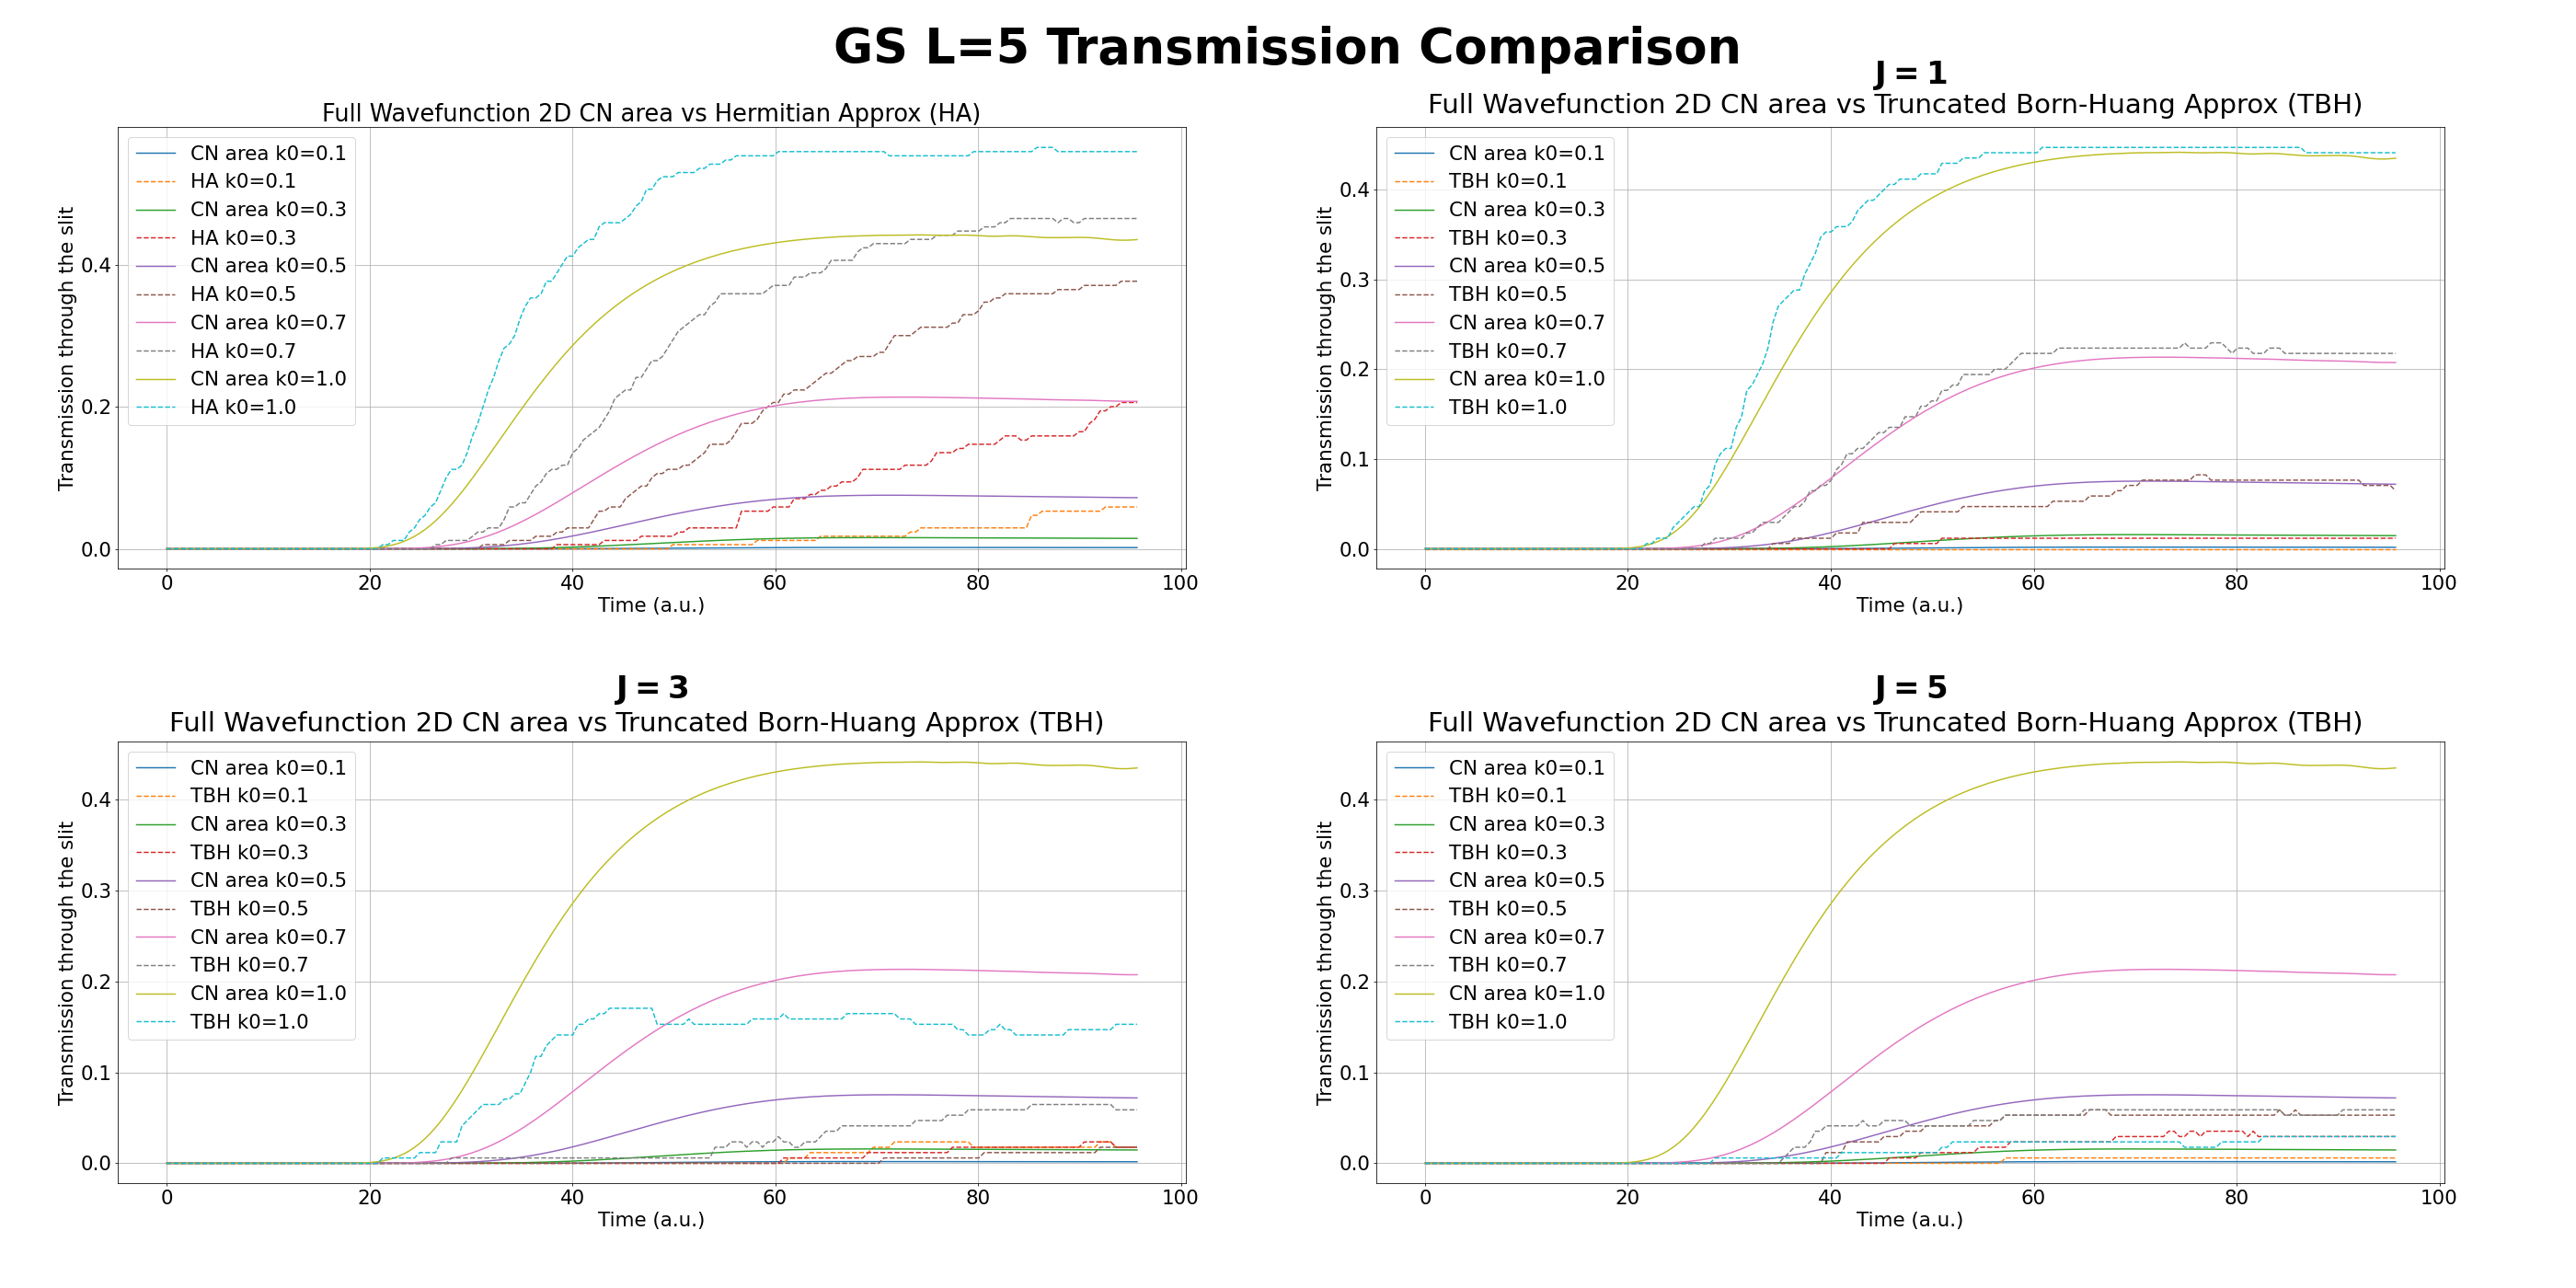
\includegraphics[width=\linewidth]{Example_Results/GS_L_5_transmission.png}
    %\caption{GS J=5 L=5}
  \end{subfigure}
  \begin{subfigure}[b]{1.1\linewidth}
    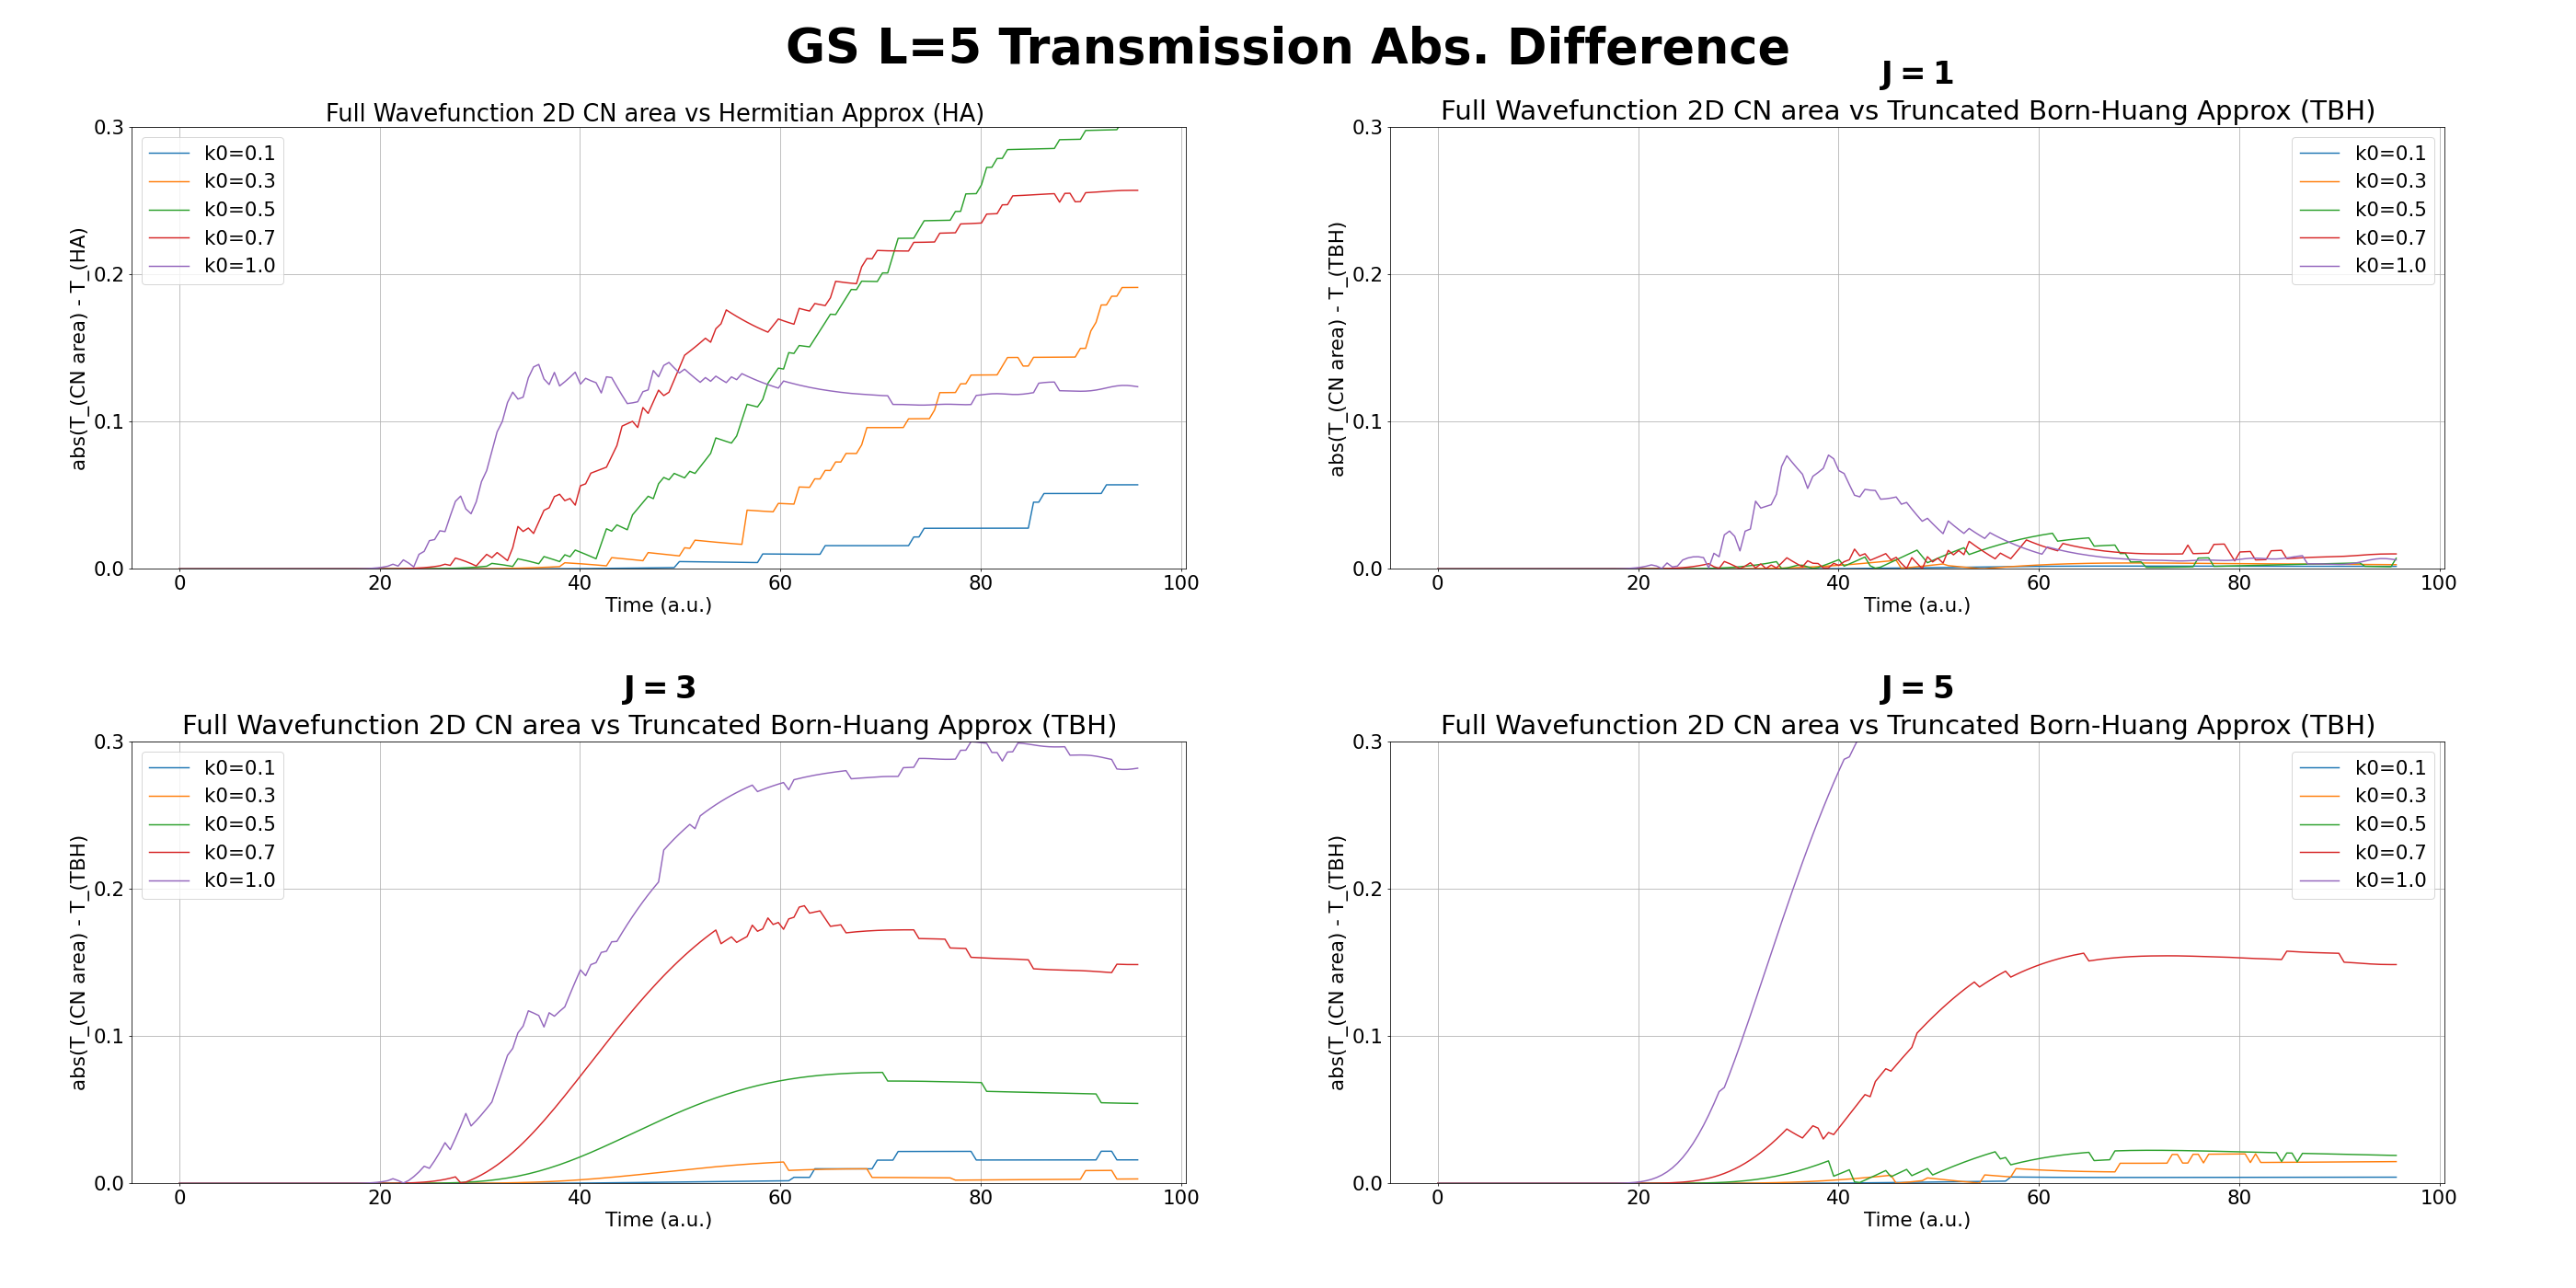
\includegraphics[width=\linewidth]{Example_Results/GS_L_5_errors.png}
    %\caption{GS J=5 L=5}
  \end{subfigure}

  
  \caption{ Transmission of the probability density computed using the full \ref{TDSE} solver Crank Nicolson compared with the transmitted trajectory proportions obtained with the Hermitian Algorithm (HA) and the Truncated Born Huang expansion algorithm (TBA), for the GS initial wave-function using $J\in\{1,3,5\}$ and $L=5$. }
  \label{fig:transm_GS_L5}
\end{figure}

\begin{figure}[p]
  \centering
  \begin{subfigure}[b]{1.1\linewidth}
    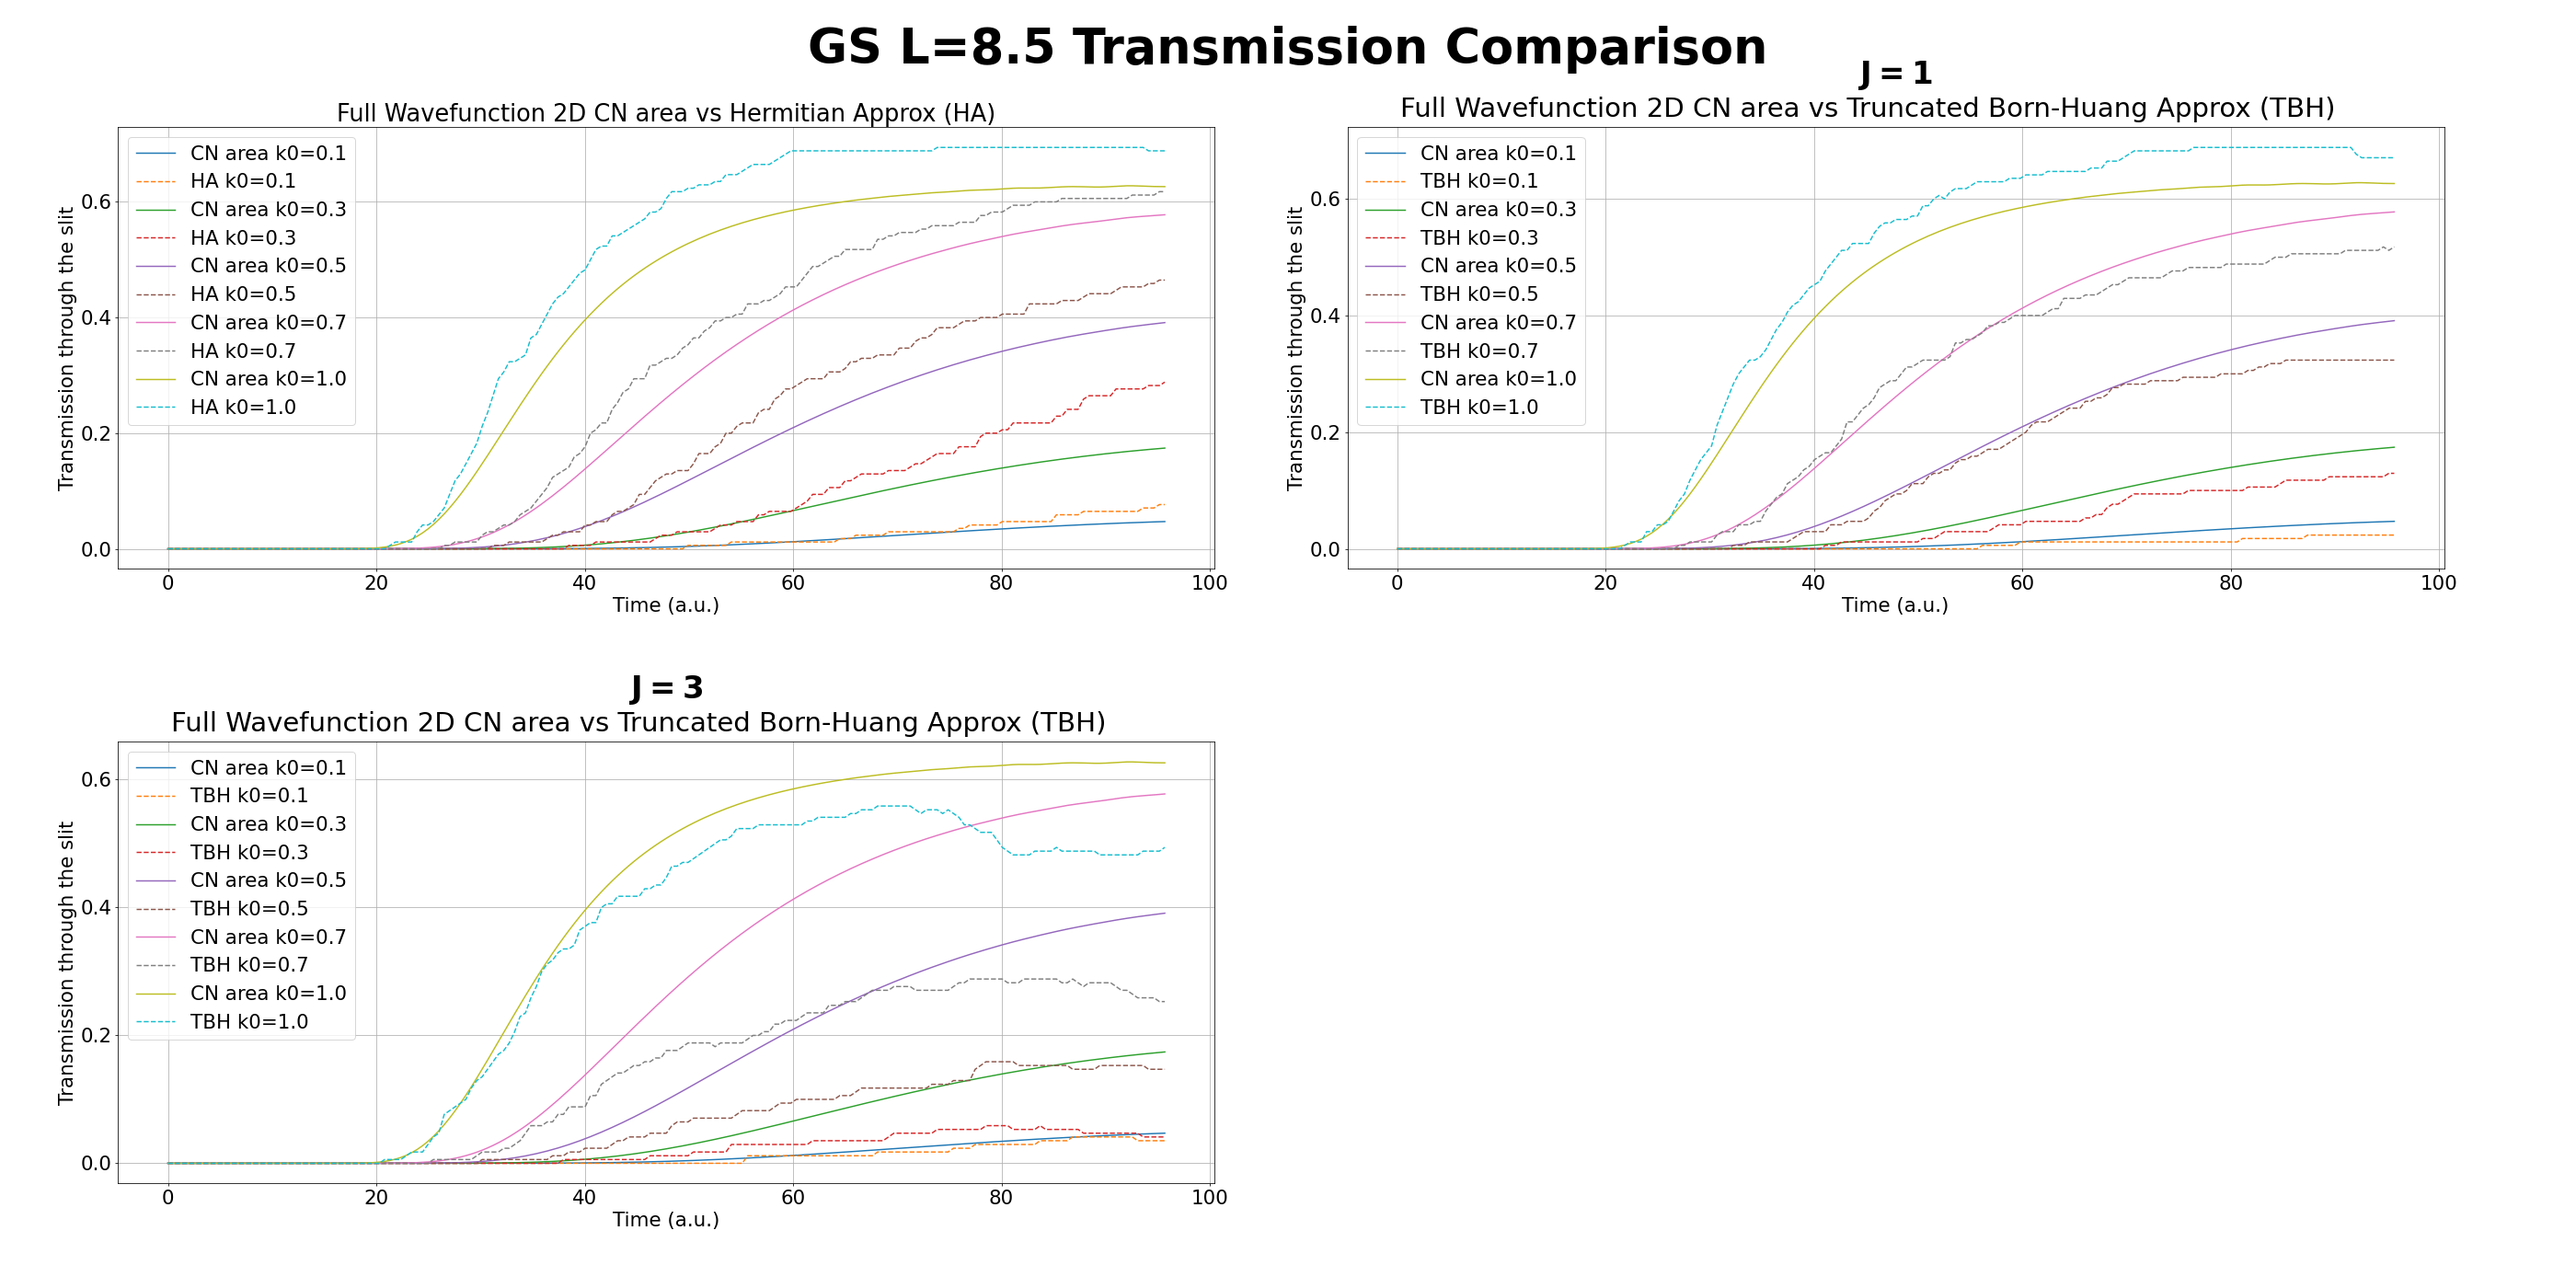
\includegraphics[width=\linewidth]{Example_Results/GS_L_8.5_transmission.png}
    %\caption{GS J=5 L=5}
  \end{subfigure}
  \begin{subfigure}[b]{1.1\linewidth}
    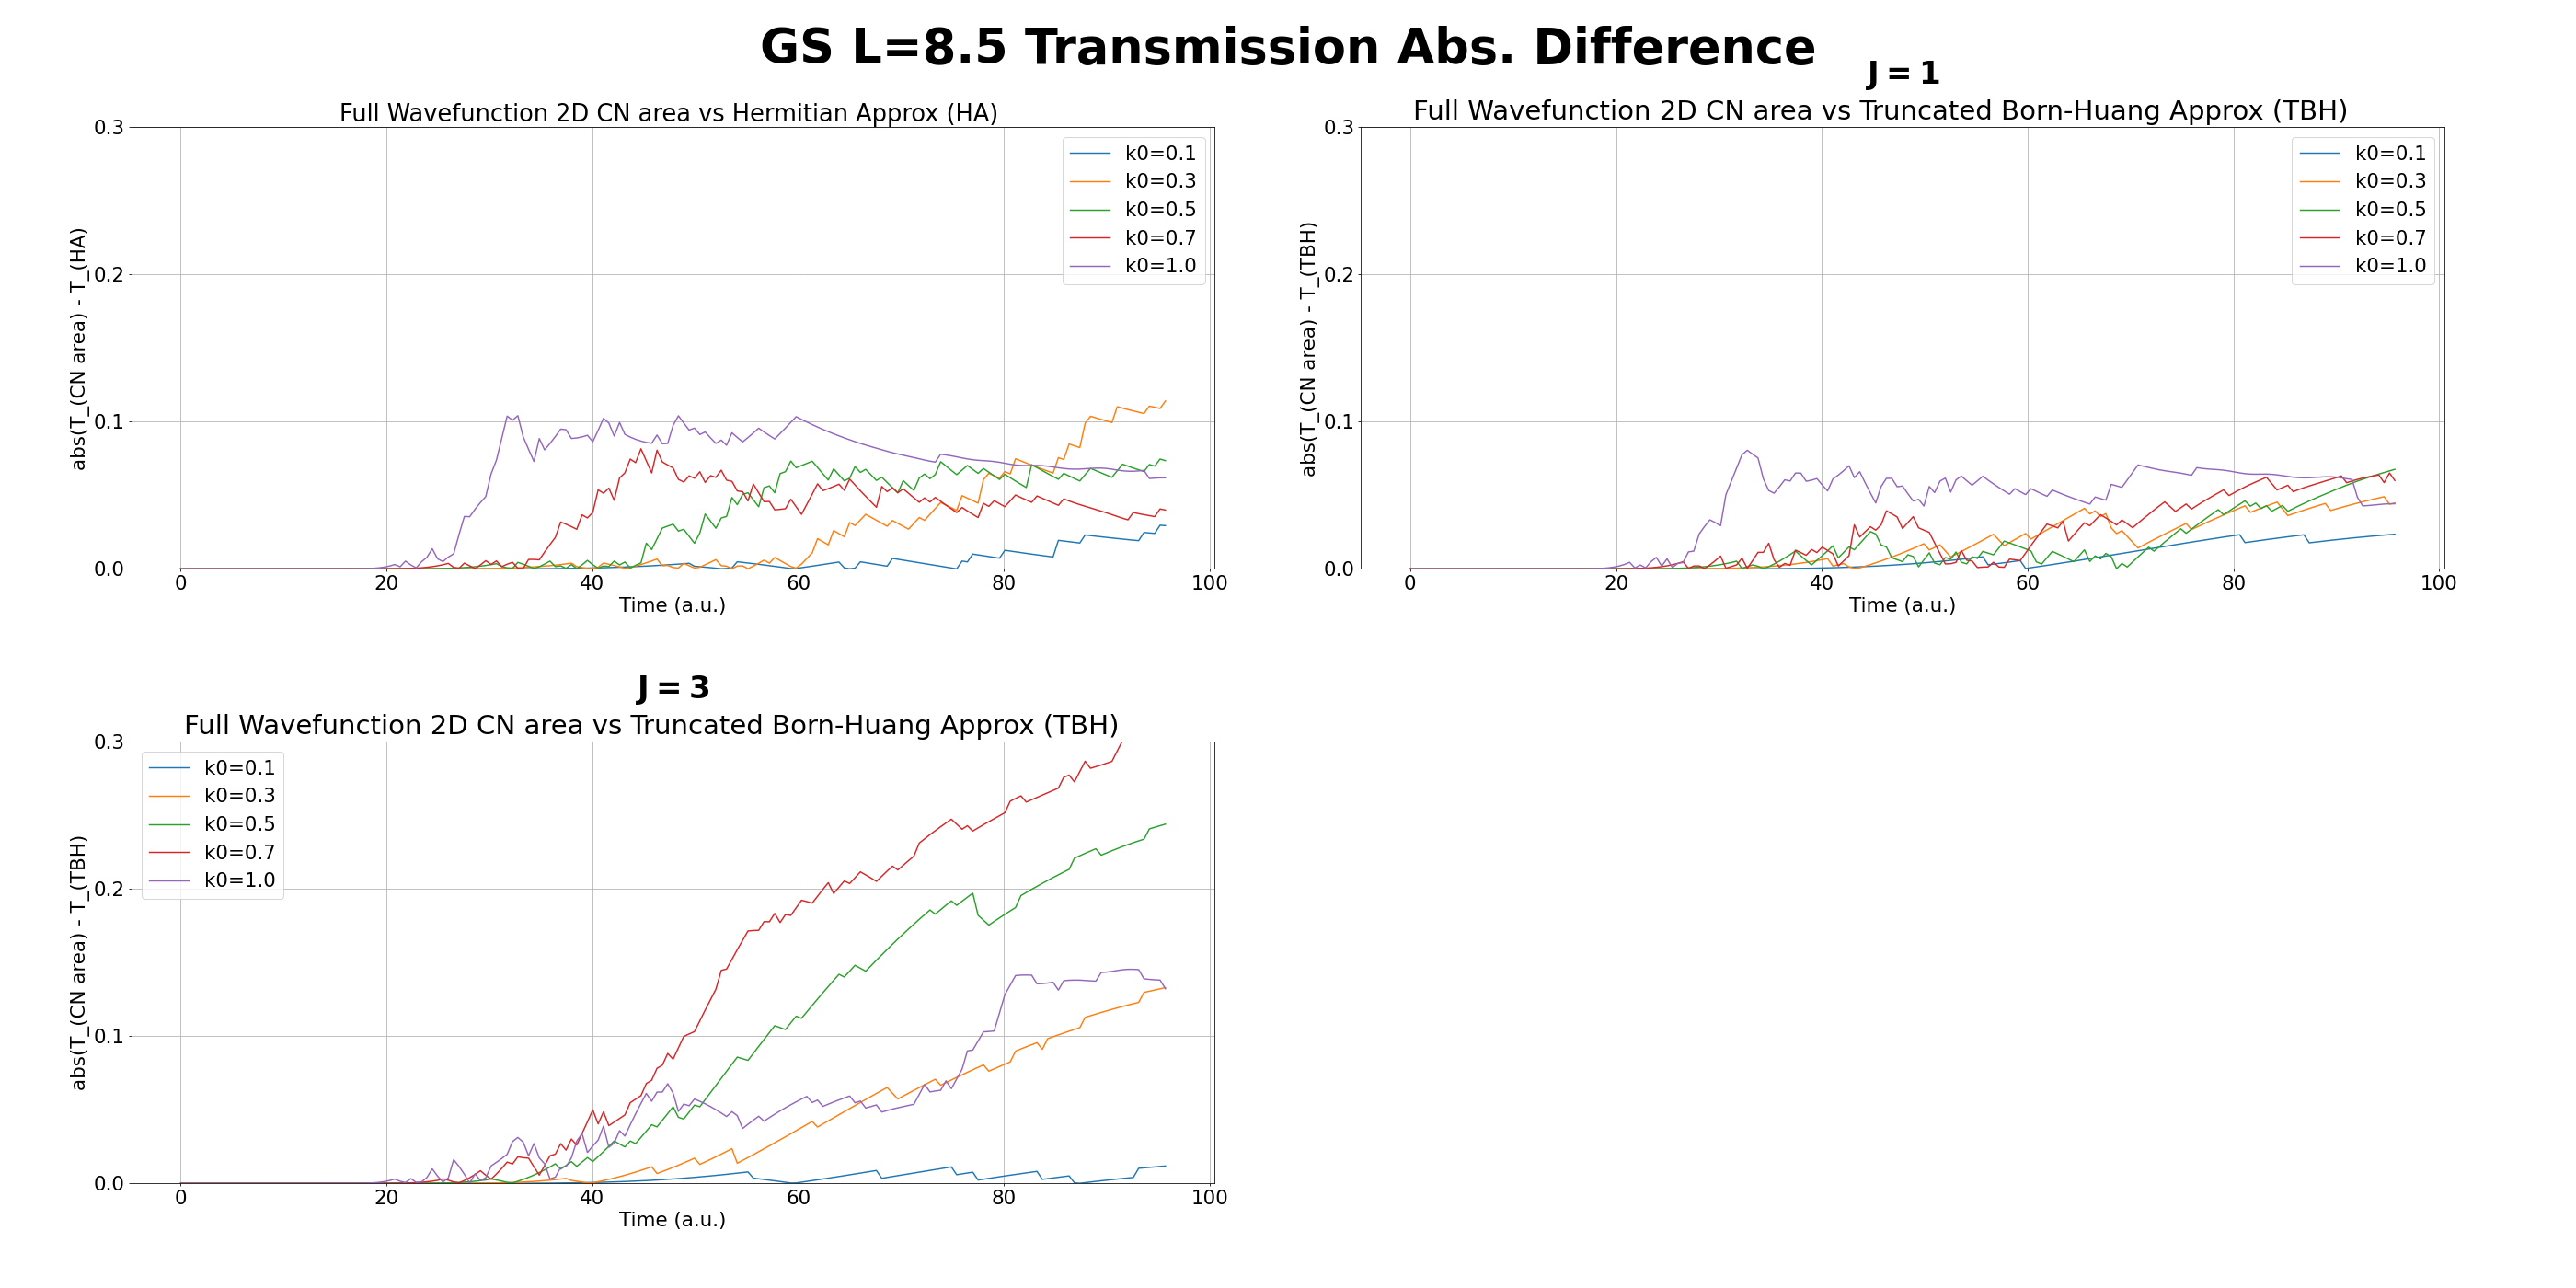
\includegraphics[width=\linewidth]{Example_Results/GS_L_8.5_errors.png}
    %\caption{GS J=5 L=5}
  \end{subfigure}

  
  \caption{ Transmission of the probability density computed using the full \ref{TDSE} solver Crank Nicolson compared with the transmitted trajectory proportions obtained with the Hermitian Algorithm (HA) and the Truncated Born Huang expansion algorithm (TBA), for the GS initial wave-function using $J\in\{1,3\}$ and $L=8.5$. }
  \label{fig:transm_GS_L85}
\end{figure}

\begin{figure}[p]
  \centering
  \begin{subfigure}[b]{1.1\linewidth}
    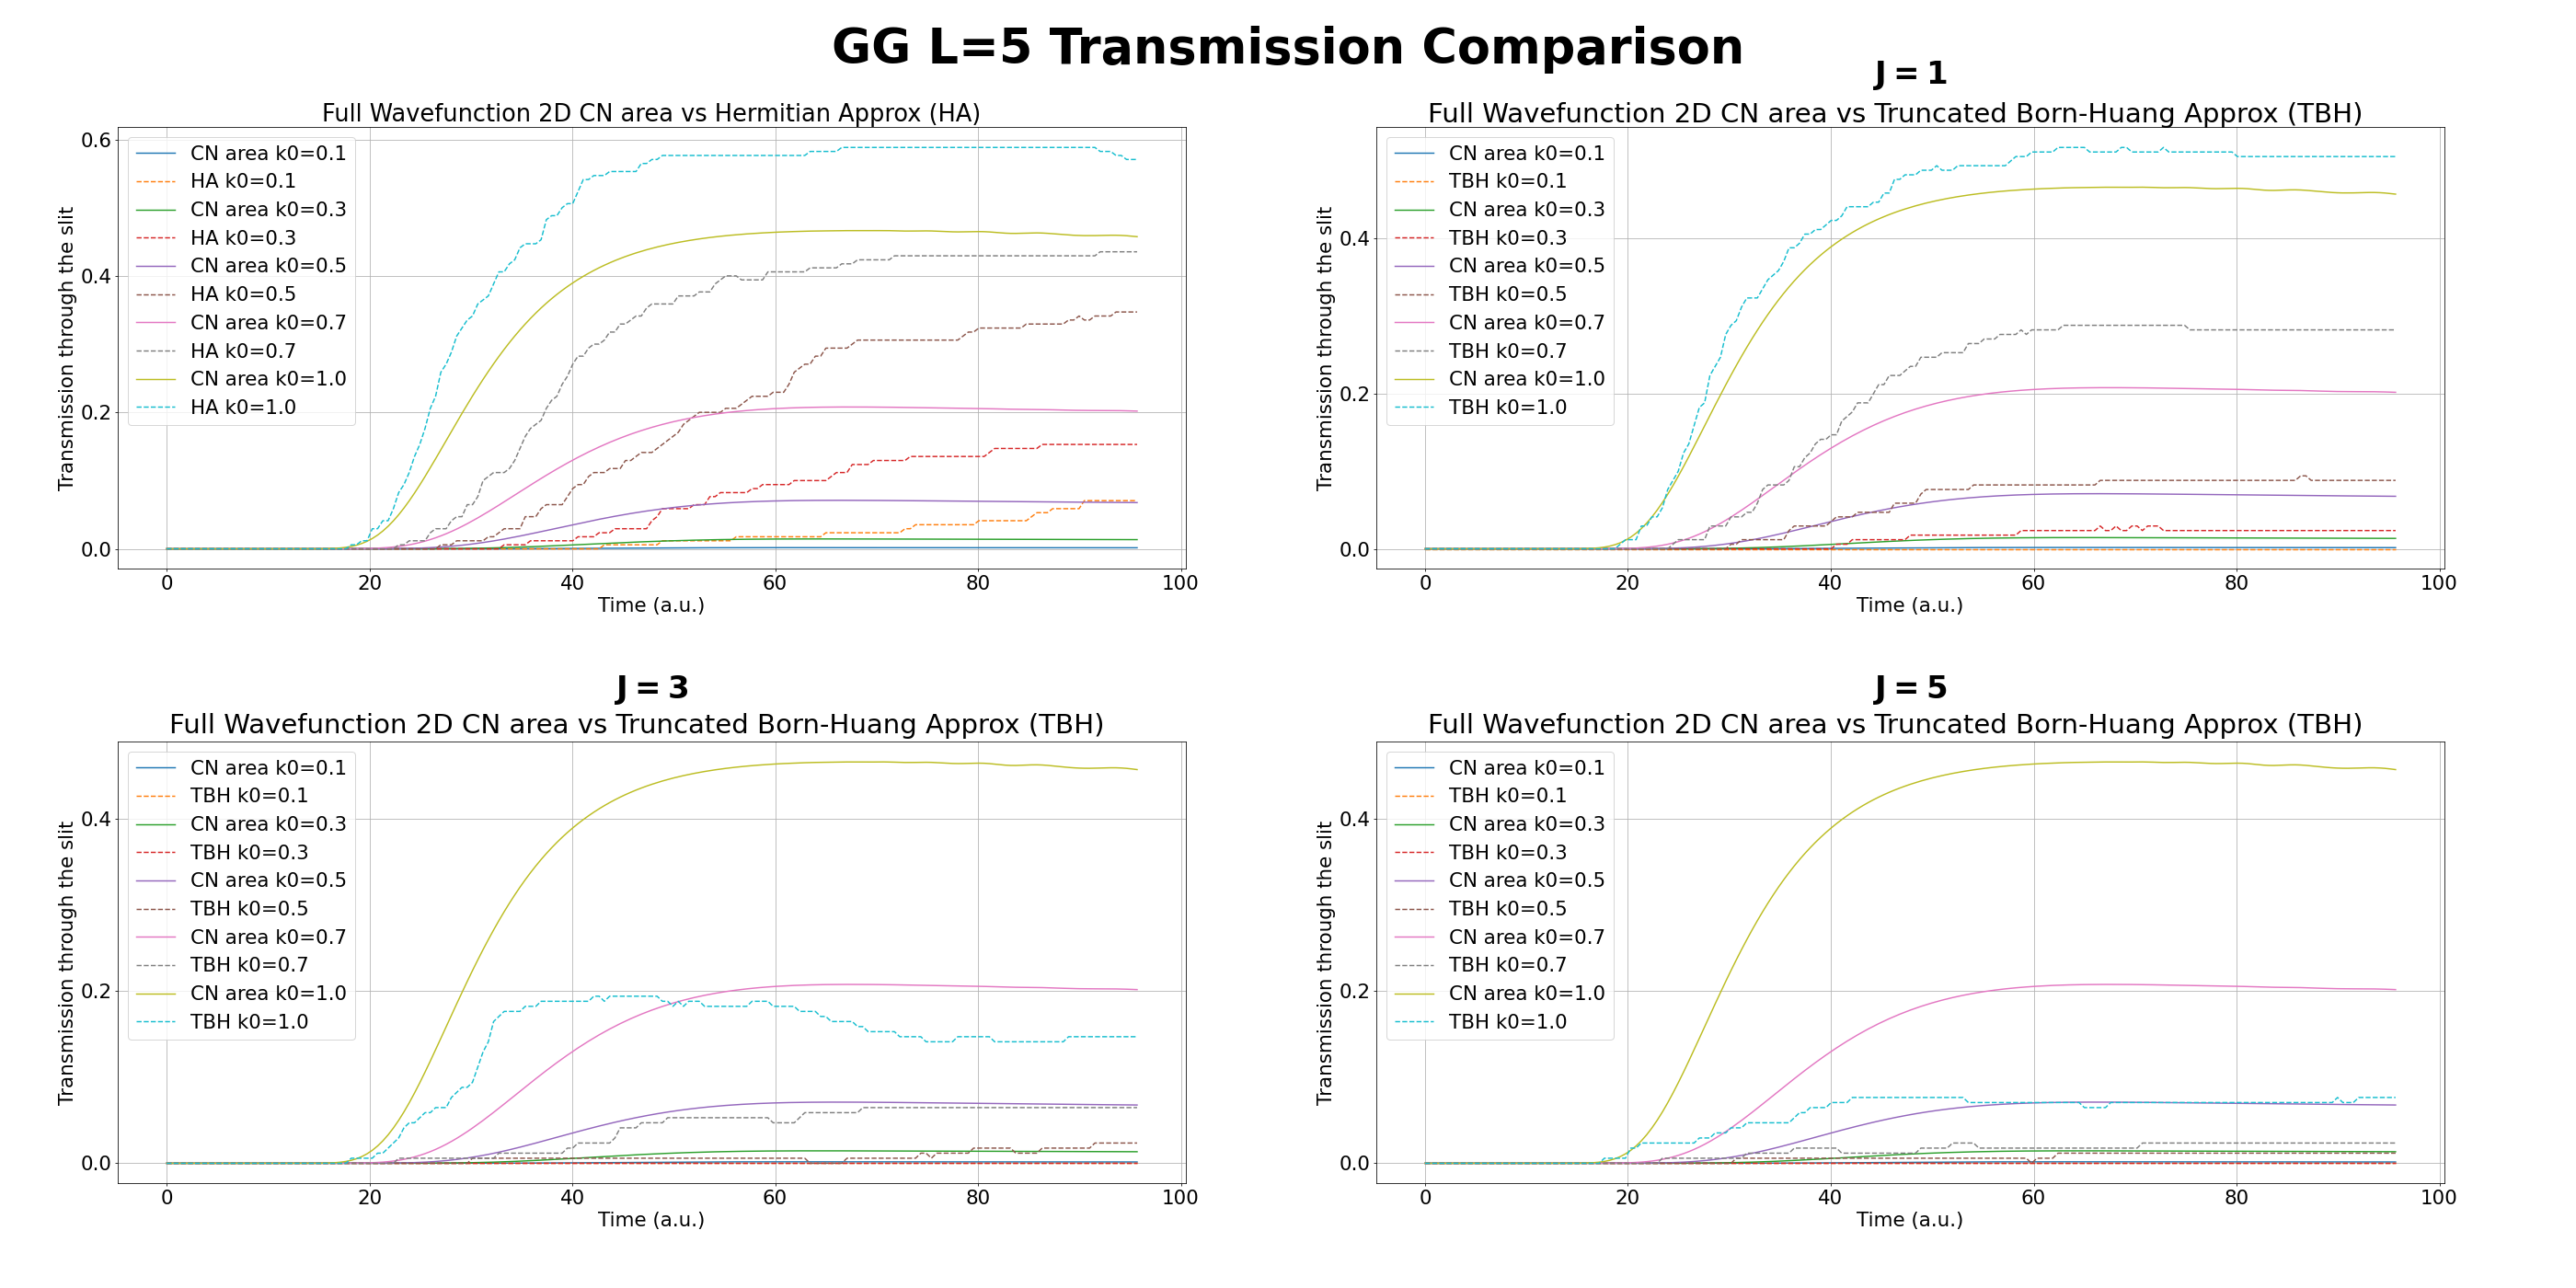
\includegraphics[width=\linewidth]{Example_Results/GG_L_5_transmission.png}
    %\caption{GS J=5 L=5}
  \end{subfigure}
  \begin{subfigure}[b]{1.1\linewidth}
    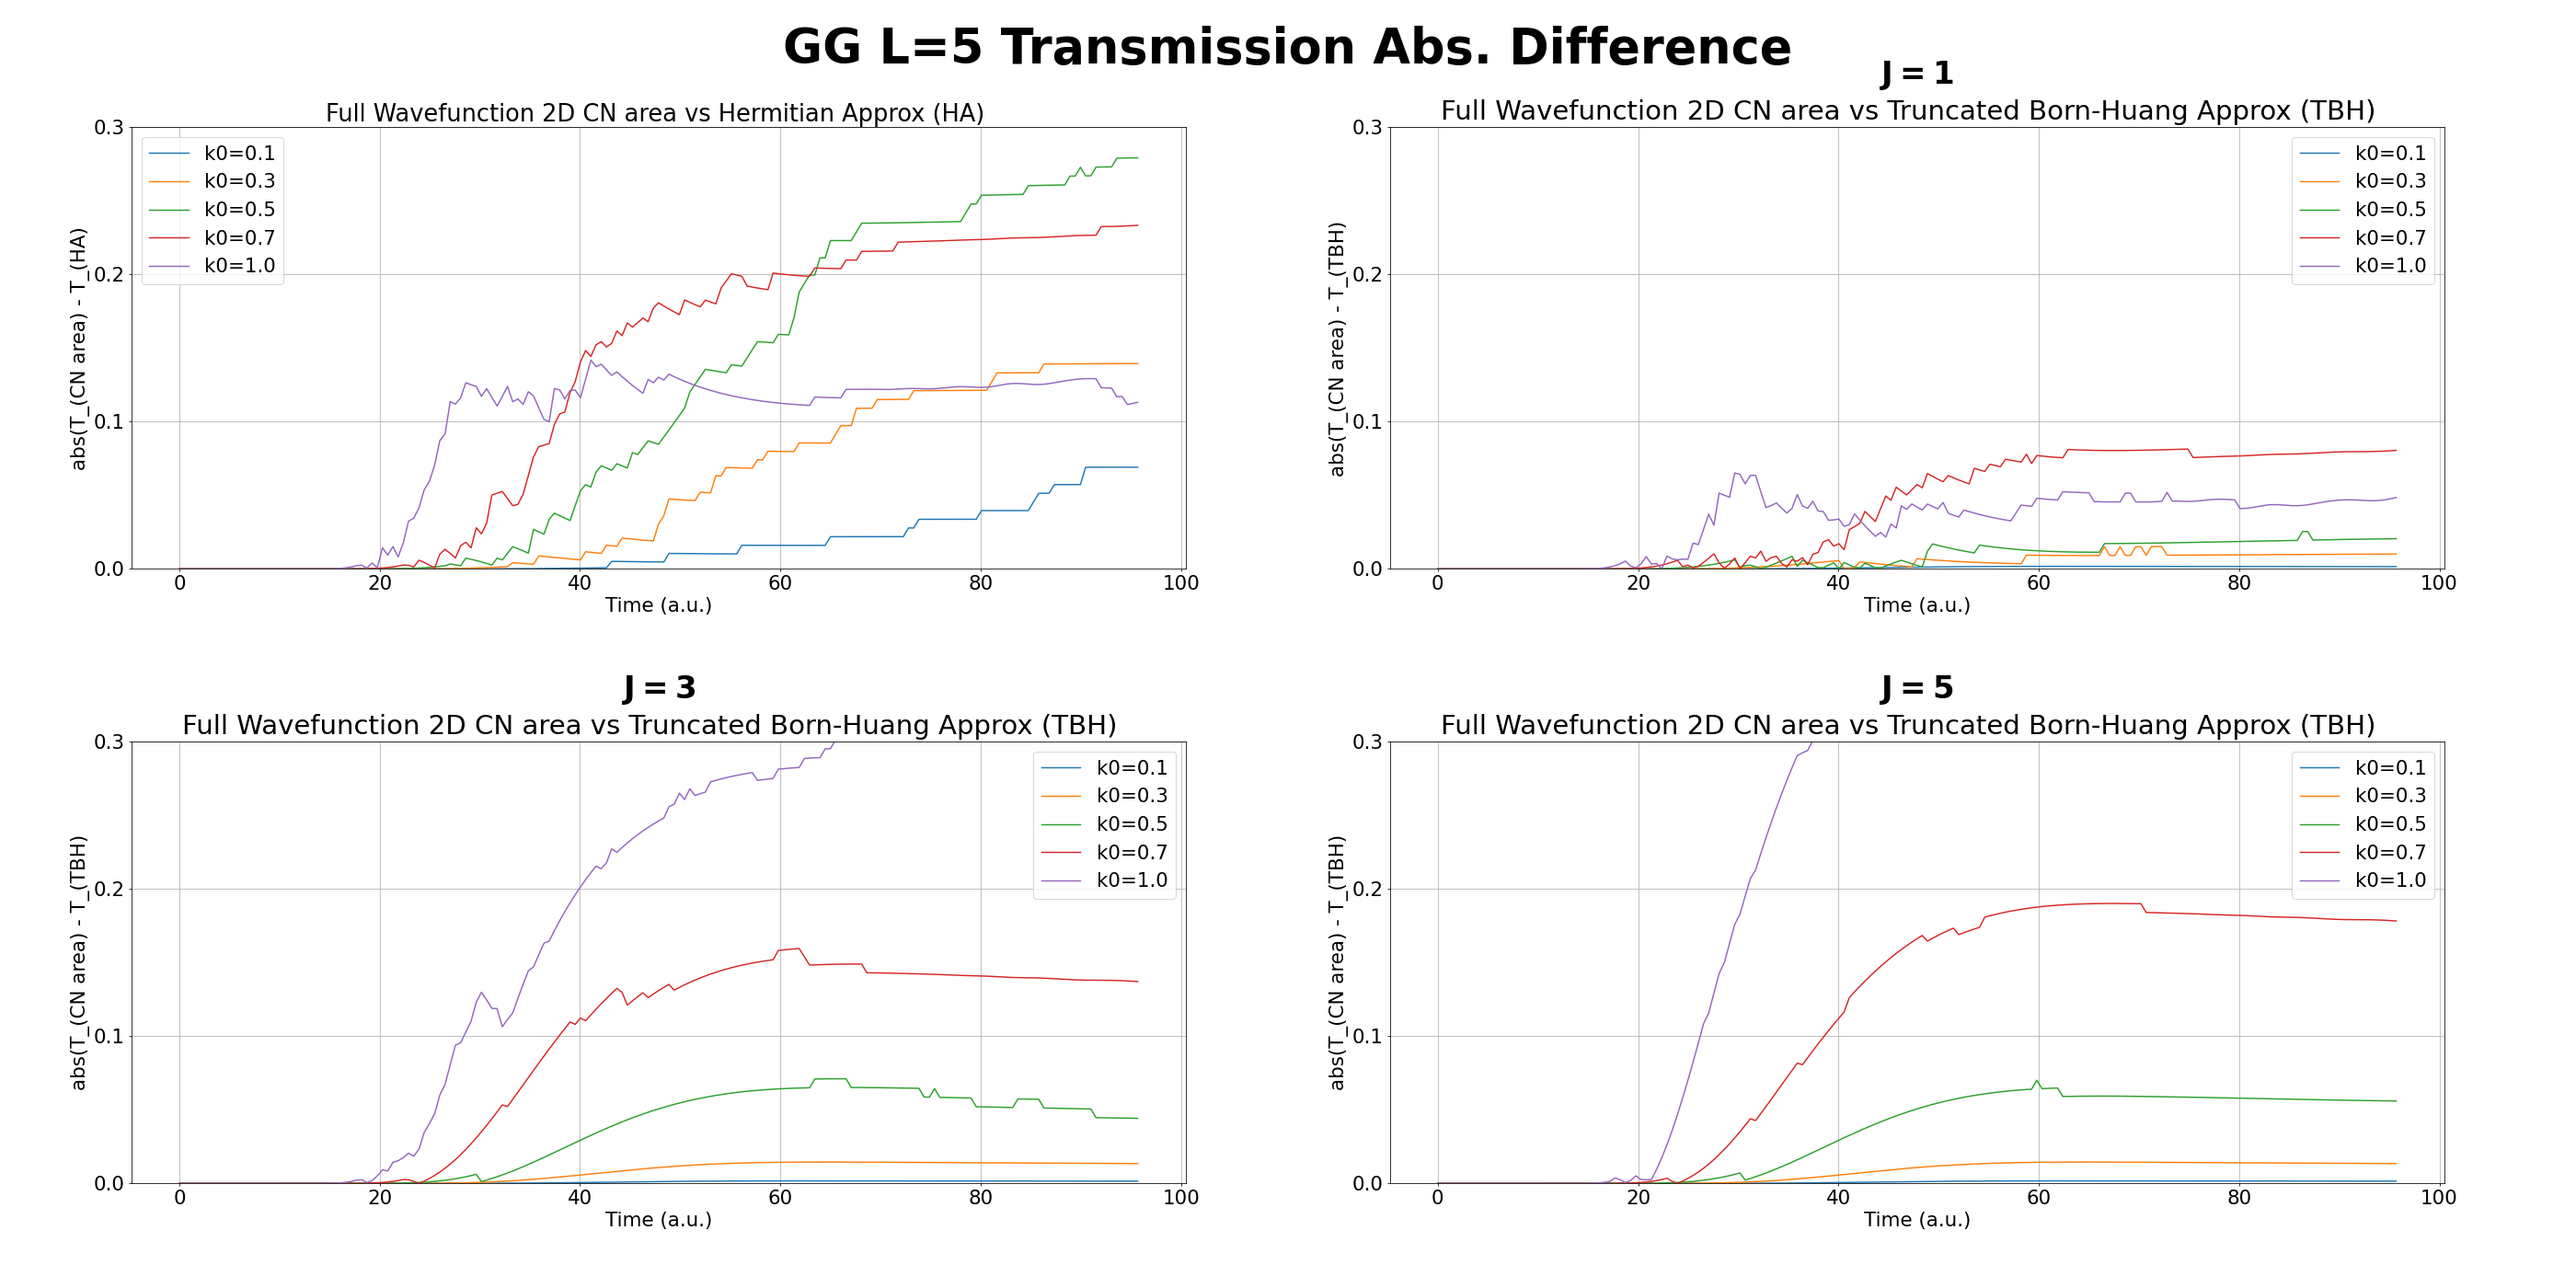
\includegraphics[width=\linewidth]{Example_Results/GG_L_5_errors.png}
    %\caption{GS J=5 L=5}
  \end{subfigure}

  
  \caption{ Transmission of the probability density computed using the full \ref{TDSE} solver Crank Nicolson compared with the transmitted trajectory proportions obtained with the Hermitian Algorithm (HA) and the Truncated Born Huang expansion algorithm (TBA), for the GG initial wave-function using $J\in\{1,3,5\}$ and $L=5$. }
  \label{fig:transm_GG_L5}
\end{figure}

\begin{figure}[p]
  \centering
  \begin{subfigure}[b]{1.1\linewidth}
    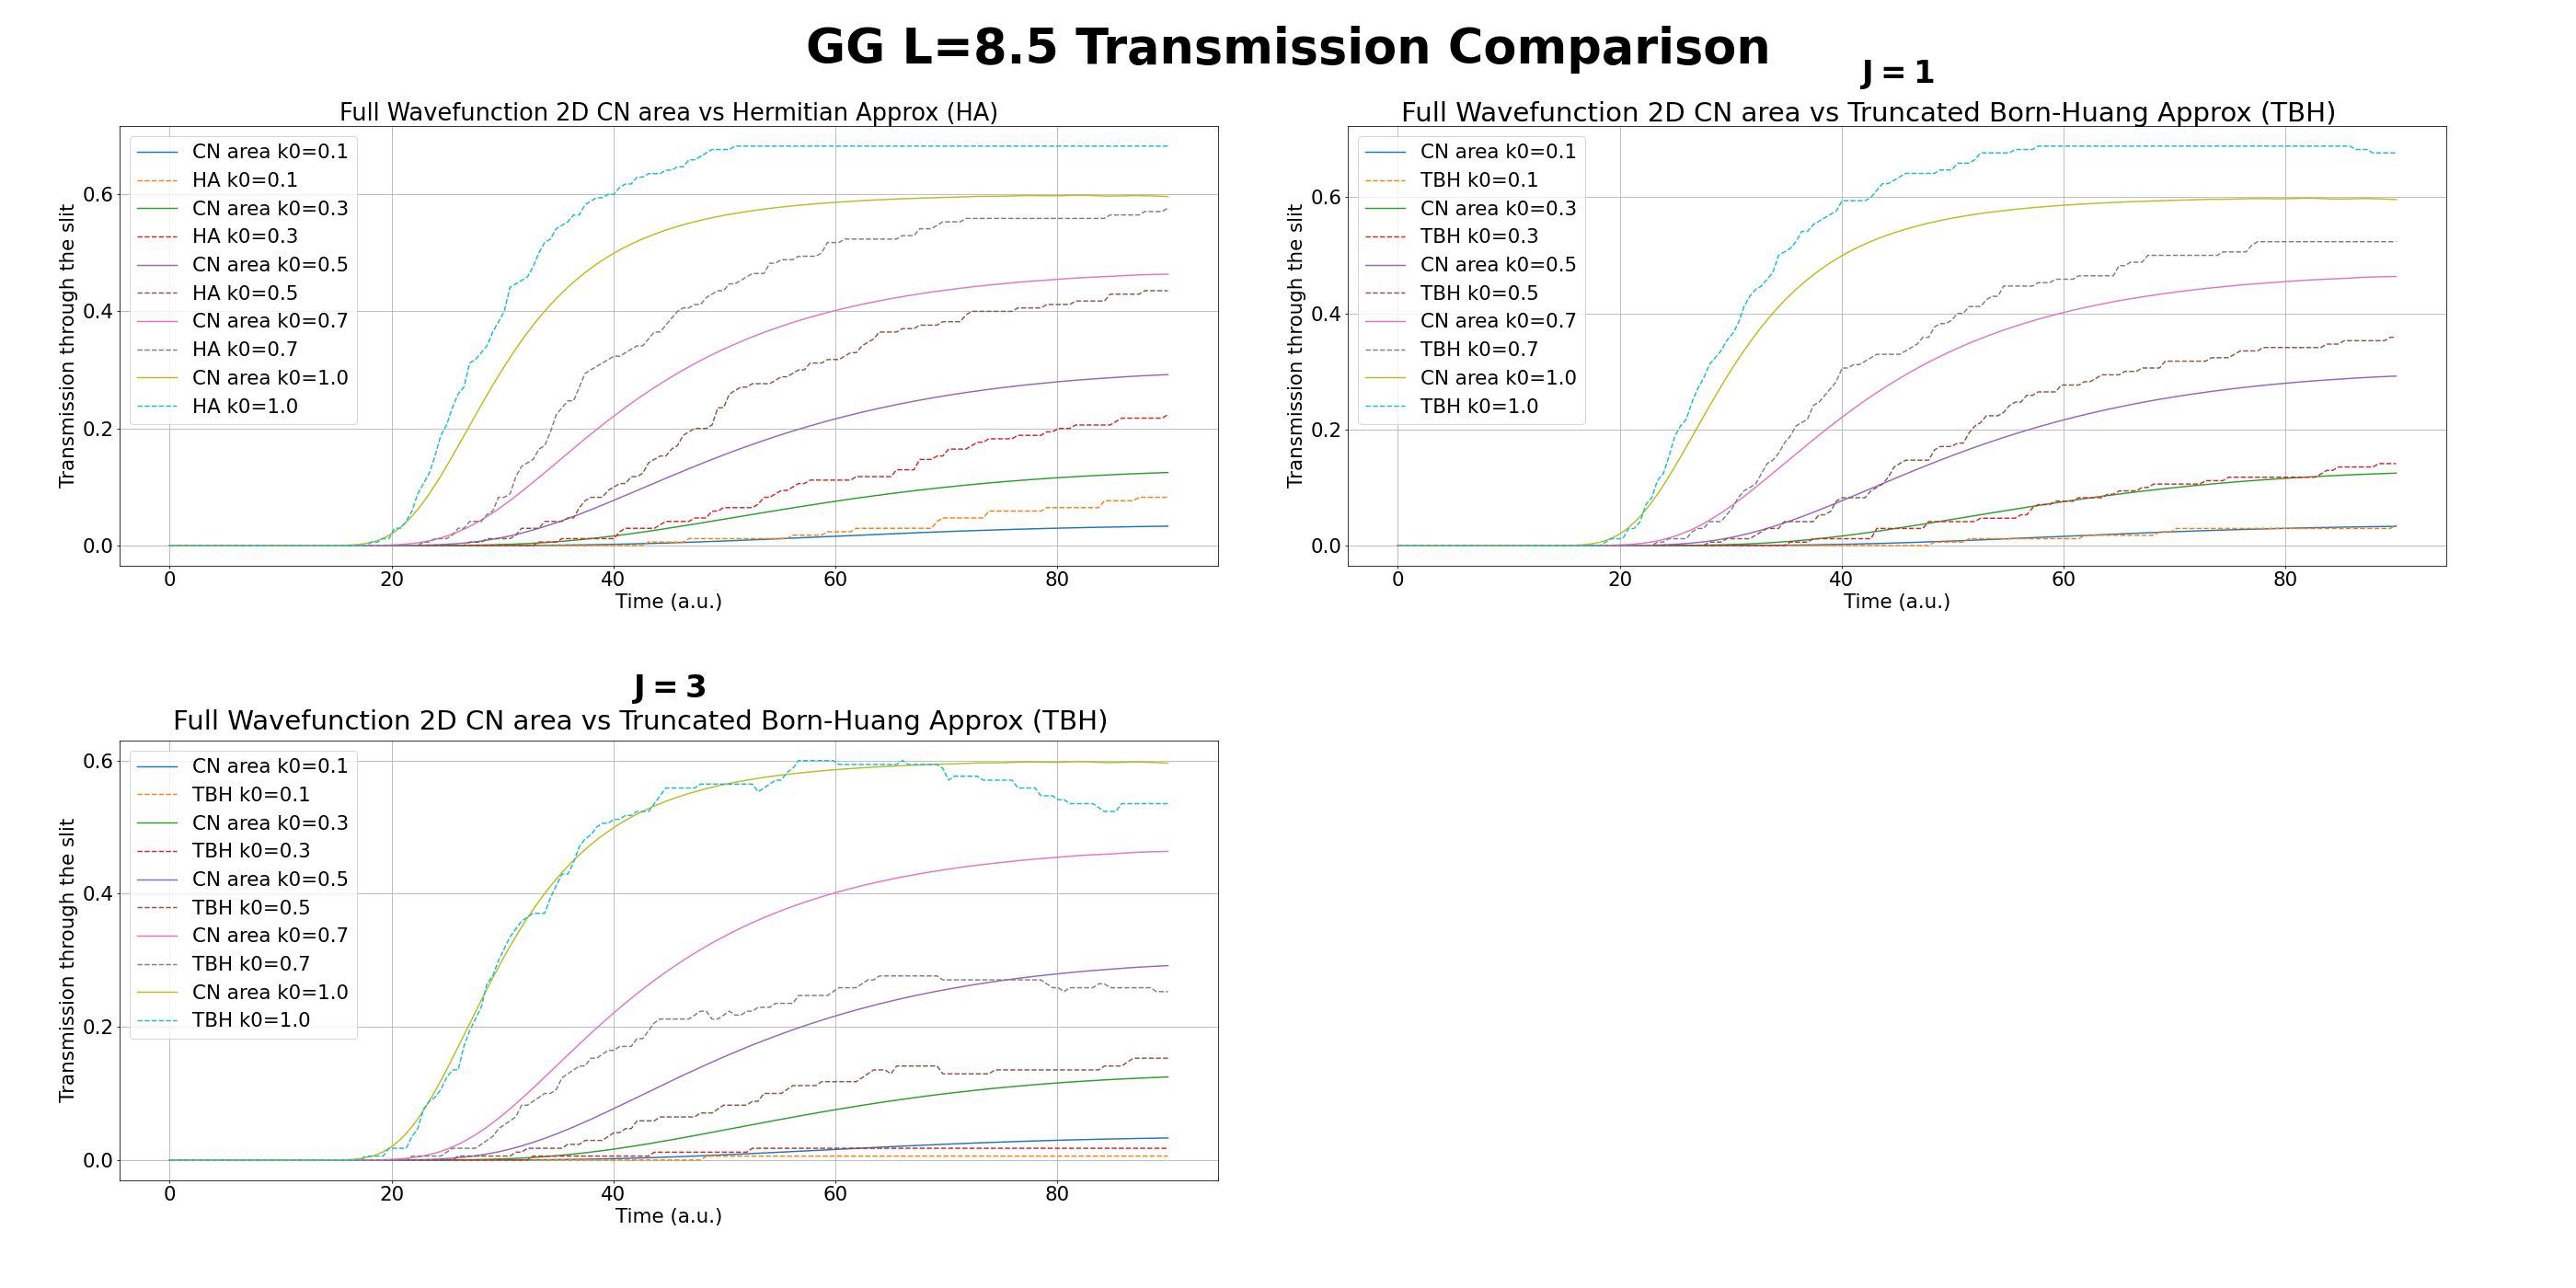
\includegraphics[width=\linewidth]{Example_Results/GG_L_8.5_transmission.png}
    %\caption{GS J=5 L=5}
  \end{subfigure}
  \begin{subfigure}[b]{1.1\linewidth}
    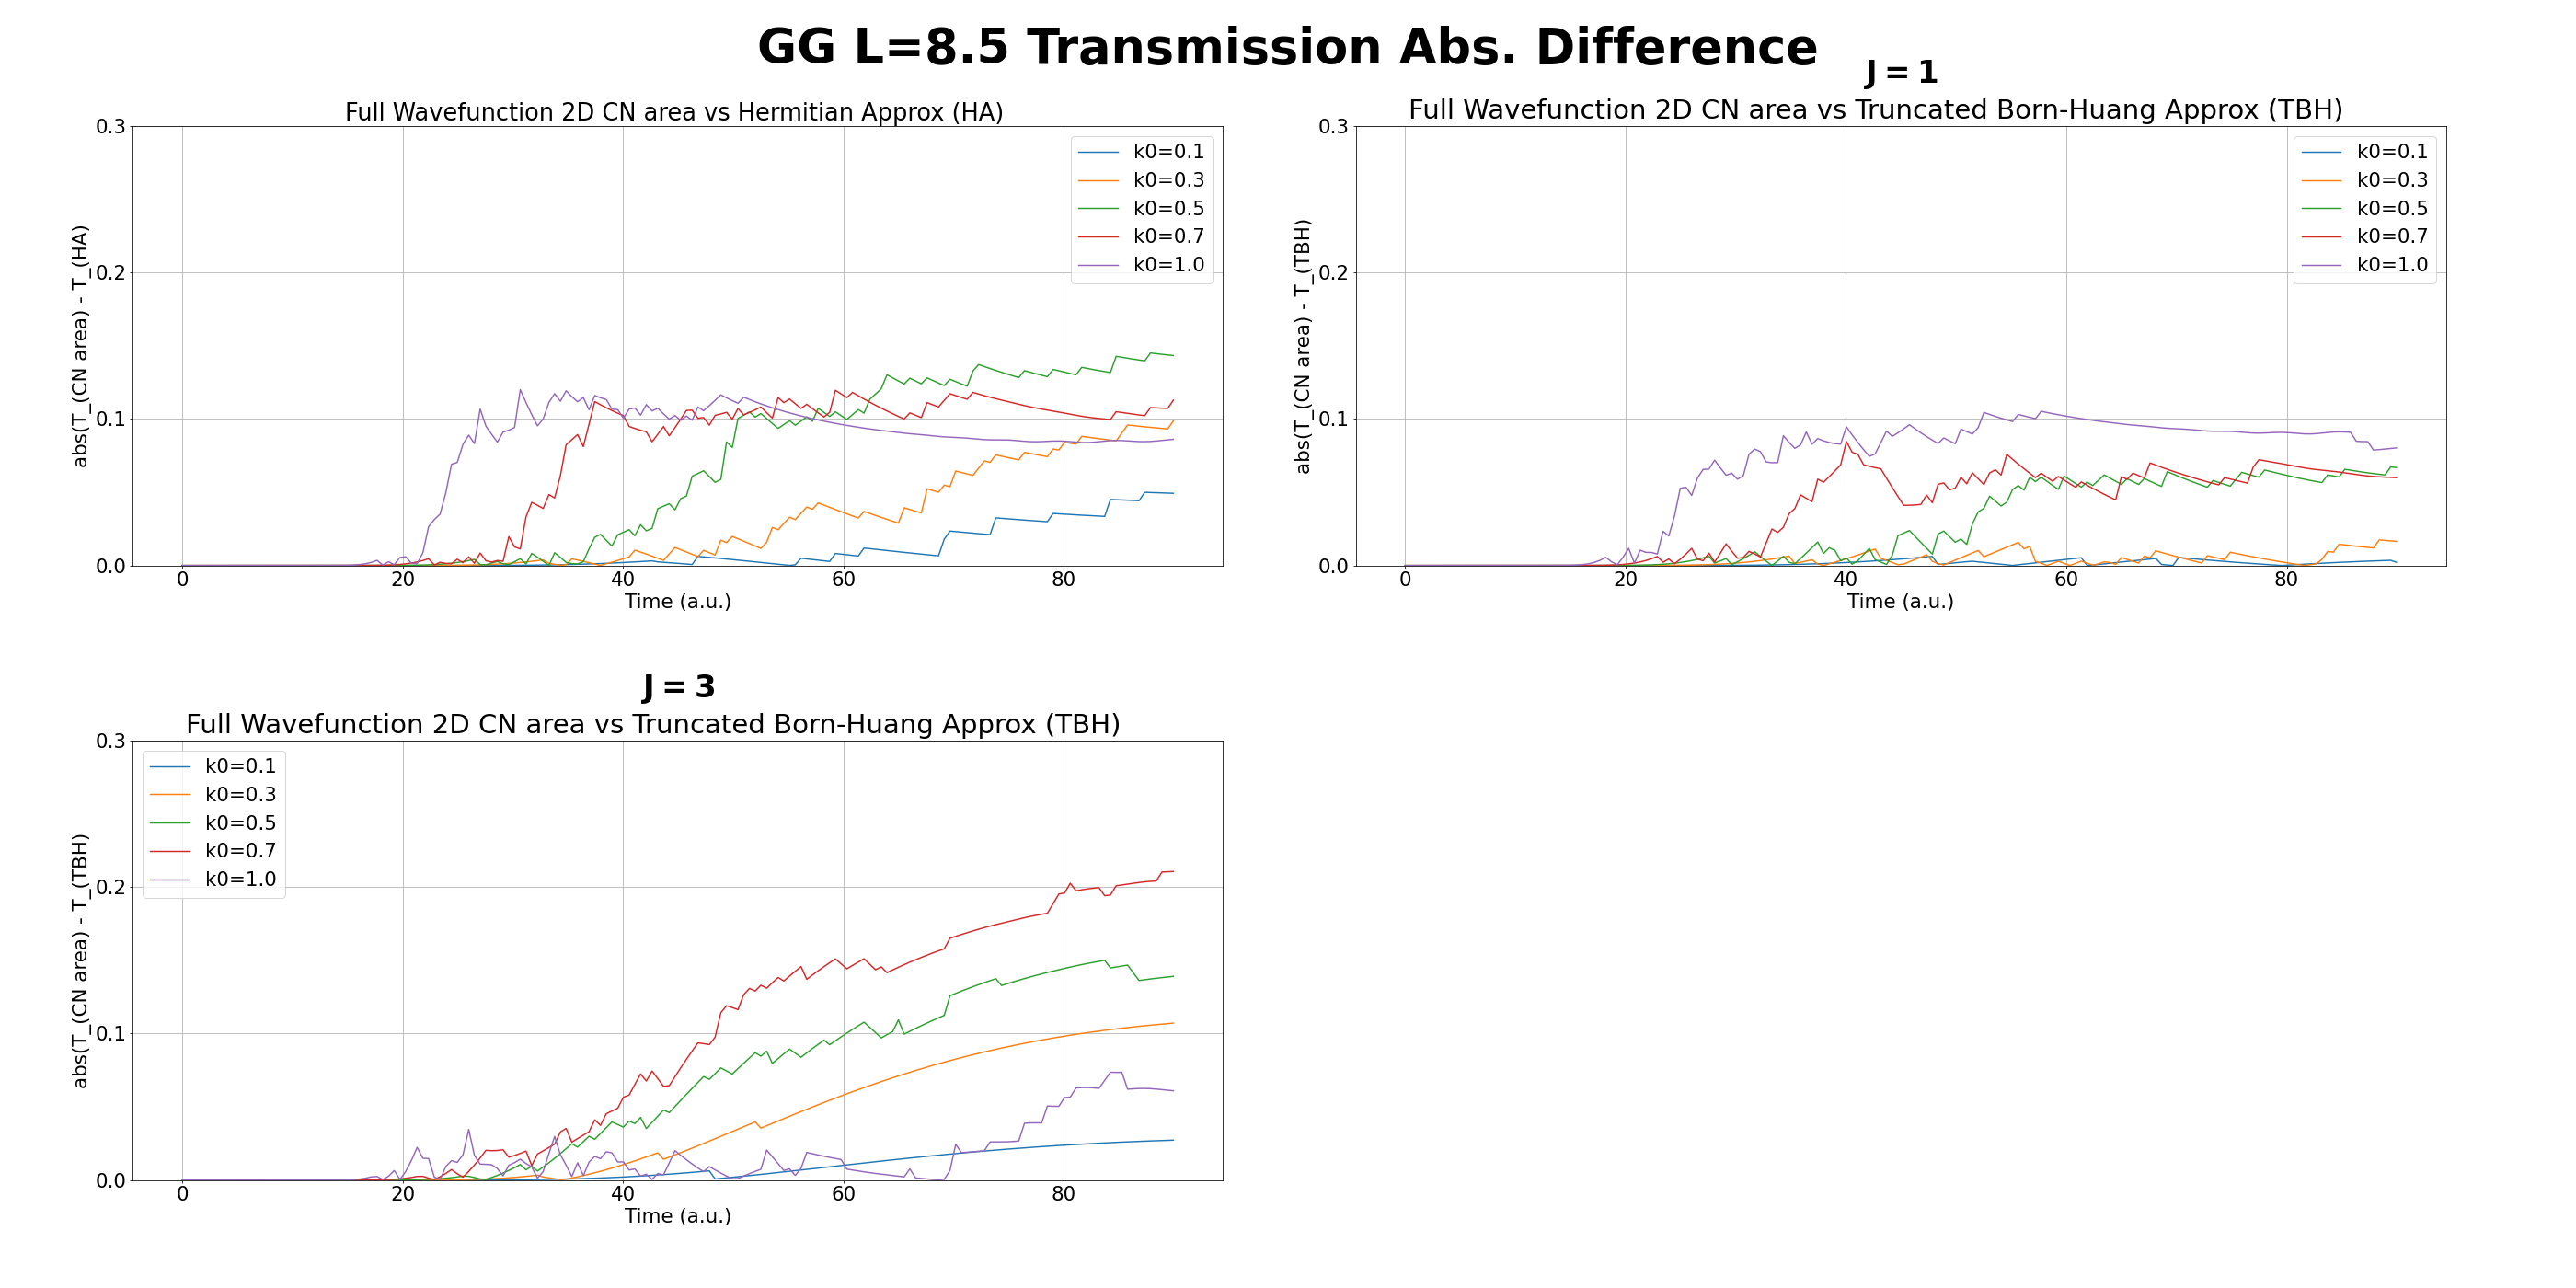
\includegraphics[width=\linewidth]{Example_Results/GG_L_8.5_errors.png}
    %\caption{GS J=5 L=5}
  \end{subfigure}

  
  \caption{ Transmission of the probability density computed using the full \ref{TDSE} solver Crank Nicolson compared with the transmitted trajectory proportions obtained with the Hermitian Algorithm (HA) and the Truncated Born Huang expansion algorithm (TBA), for the GG initial wave-function using $J\in\{1,3\}$ and $L=8.5$. }
  \label{fig:transm_GG_L85}
\end{figure}

{\em Simulations for GS L=5 J=3 and J=5, together with those for GS L=8.5 and GG L=5, L=8.5 (each for J=1,3,5) are still running and will probably take about two and a half weeks to be ready. However, with this first result we can be more than happy I believe!}

{\em To be continued...}

% explike konceptoa transmisiñoa neurtzie dala traiektorixek erabilitte ta kompare exkatoagaz eta bi aproximaziñoak. 
% Erakutsi transmisiño plotak eta ikusi zelan eztanien egon biher transmisiñorik eztauen eta biher danien bai
% obserbe zelan J altuaue txrraue dan puntu batetik aurrera Hermitiannen antzekoaue dalako. Komente bebeia ia 2gaz ondo badoan populaziñoa bigarren eigenstateien tal o cual dalako. Igual integre ein biherkjo naben populaziñoa estado bakoitzien ikusteko denporan ziher zelan doan aldatzen.







%g=1.0,a1=0.0,a2=12.0,Lmax=40.0,Lmin=7.0,L1; L1= (Lmax-Lmin)/2.0*(1.0/(1.0+exp((x-a1)/g))+1.0/(1.0+exp((-x+a2)/g)))+Lmin/2.0; if(y>L1 || y<-L1){return 100.0;} else{return 0.0;}
% Ze complex potential geratzen da other than the Hermitian approx
% Ze ifektu deko termino bakoitzak. Zerba bakarrik itxizgero Kren aproximaziñoa good enough dan
% Ein explikaziñoa goiko sekziñoan zegaotzik en si ezin dan generalize ah expresiñoa, ze ya trukoa ezta egixe, baia bueno trampa eitzen bazun ba tal.
% saiatu ondo idazten igual gehitzen ta kentzen potentzixela. Bia bueno argi txi ezin dozun bitartien atara psitik beste psi bat u ta jotakaz U eztala inogaz ikusiko.
% oin hona buelteta esan zerba hemen kasuen funtzionetan deuen - U=0 dalako hor barruen basikamente


%Sartun plota potentzixelana jarritte zelan alzun kontroleu adiabaticidadie ta eigenstatek.
% Ein tabla bat de wavepacket energy eta tseig energies ta erakutsi transmisiñoa full SEenana against 150 trayektoria con Hermitian eta con el nuestro con j= tal j= cual.
% ta honen ostien ein desarrollo bat de ekuaziñoak ze forma hartzen dabien j=1egaz eta bestiekaz 
% Ta falte dan beste gauzie da en generaleko termino haretan lenguaje d elos chiserako bidie pavie holan gero hemen alzu cite direktamente kasu partikular modure.




\newpage
\section{Reconstructing the Full Wave-Function from CWF-s}
% Idatzi algoritmoa baia ipini generiko moduen aprox de G,Jgaz
Apart from the ontological interest that these algorithms could have, where only one Bohmian trajectory and its associated CWF-s are evolved at each run, the observed results in quantum mechanics still are randomly found among the ensemble of possible trajectories. As such, the ensemble measurements are the most interesting for orthodox quantum mentality and perhaps quantum information and computation, at least as far as we cannot get rid of the probabilistic nature of the observation. Therefore, it seems clear that if the many-body problem can be educatedly surpassed in the computation of individual Bohmian trajectories and CWF-s as defined in (\ref{CWF}), we should try to take advantage from it to approach an approximate solution for the full wavefunction (which in reality contains information about all the possible trajectories and associated CWF-s). But how to do this?

Let us review what is the information we have, once an approximate solution to any of the shapes of the \hyperref[CWF.SE]{(CWF.SE)} is found, and see if we can build something from there:
\begin{enumerate}
\item[(a)] Given a bounded time domain $t\in [t_0,t_f]$, we know $\Psi(\vec{x},t=t_0)$, the full wave-function at the first time, and $U(\vec{x},t)$ $\forall t\in[t_0,t_f]$, all of which were given a priori by the user or the problem we are facing.

\item[(b)] We will have chosen $M$ initial positions in configuration space $\{\vec{x}^\beta(t_0)\}_{\beta=1}^M$ by sampling them as independent observations from the initial wave-function, using its interpretation as probability density of possible experimental outcomes $\rho(\vec{x},t_0)=\Psi(\vec{x},t_0)^\dagger \Psi(\vec{x},t_0)$. Using each of the $M$ trajectories, we will have defined the set of $N$ conditional wave-functions (CWF) related to each as:
$$
\qty{\qty{ \psi^\beta_a(x_a,t_0)\equiv\Psi(x_a,\vec{x}_b^\beta(t_0),t_0)}_{a=1}^N}_{\beta=1}^M
$$

\item[(c)] If we are to use the Born-Huang ansatz, we will have calculated numerically or analytically the transversal section eigenstates $\qty{ \qty{ \Phi_a^j(\vec{x}_b,t)}_{j=0}^{J_a}}_{a=1}^N$, following equation (\ref{TSEig}).

All (a), (b) and (c) will be as exact as finite precision arithmetics and the numerical eigensolver allow us. In principle no theoretical approximations on them.

\item[(d)] Then, by using an approximation to one of the shapes of (\hyperref[CWF.SE]{CWF.SE}), we will have obtained an approximation of the following functions: \begin{itemize}
\item The $M$ trajectories: $\{\vec{x}^\beta(t)\}_{\beta=1}^M \quad t \in [t_0, t_f]$ 
\item The $MN$ CWF-s: $\qty{\qty{ \psi^\beta_a(x_a,t)}_{a=1}^N}_{\beta=1}^M \quad t \in [t_0, t_f]$ 
\item In case the Born-Huang expansion was used, the adiabatic coefficients: $$\qty{\qty{\qty{ \chi_a^j(x_a,t)}_{a=1}^N}_{j=0}^{J_a}}_{\beta=1}^M \quad t \in [t_0, t_f]$$
\end{itemize}
\end{enumerate}
So the question at this point is: isn't there any way to unify all this information that each trajectory provides us? Should we really only use the resulting Bohmian trajectories as information source, or can we exploit the information in the approximated CWF-s?
\newpage
\subsection{Using the CWF definition}
In reality, each conditional wave-function is a slice of the full wavefunction, meaning that if we had enough CWF-s (if $M$ was big enough and the trajectories were evenly enough sampled), we would effectively be also approximating the full wave-function. See Figure \ref{fig:slices} for a graphical intuition.

\begin{figure}[h!]
  \centering
    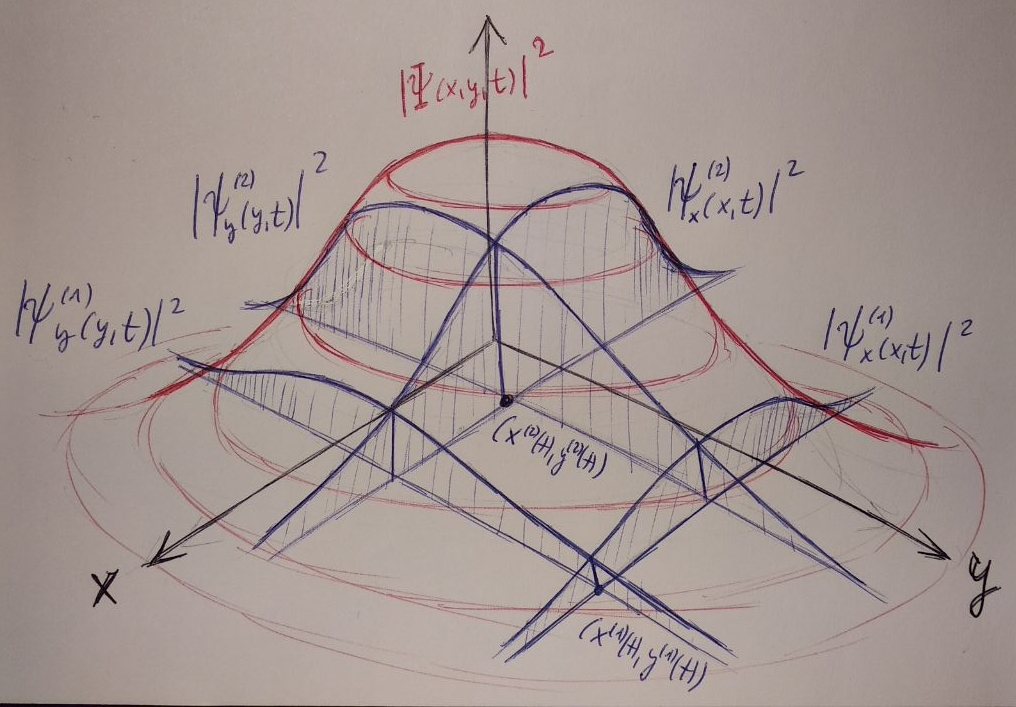
\includegraphics[width=0.65\linewidth]{slices.jpg}
  \caption{Depiction of the probability density of a 2D quantum system ($N=2$). In red the probability density of the full wave-function $\Psi(x,y,t)$ for a given time. In blue the pair of conditional wave-functions associated to two Bohmian trajectories $(x^{(1)}(t),y^{(1)}(t))$ and $(x^{(2)}(t),y^{(2)}(t))$ at a given time. Note that actually they coincide with other two trajectory's CWF-s at that time. }
  \label{fig:slices}
\end{figure}

 Now, even if our CWF-s are approximations of the true CWF-s, the value predicted around the trajectory may be expected to be one of the most accurate parts of the predicted CWF. This value, in theory should be coincident between the CWF-s, that is:
$$\Psi(\vec{x}^\beta(t),t)=\psi^\beta_1(x_1^\beta (t),t)=\cdots=\psi^\beta_N(x_N^\beta (t),t)$$ 
One could argue that stating this is the finest approximated part of the CWF is a consequence of the fact that for instance, the Hermitian approximation is compatible with a zeroth order Taylor expansion around the trajectory for $G$ and $J$. If this assumption was true, then the set of CWF-s and their associated trajectories would provide us with a dynamical grid over which we are evolving the full wavefunction. The problem with this approach would be that the number of grid points in $\R^N$, over which we are evolving the full wave-function would be equal to the number of trajectories evolved $M$, which unfortunately would need to be geometrically bigger to obtain a good enough resolution with increasing dimensions. This would therefore be avoiding us to solve the many body problem anyway. It could be argued though, that at least this way, the many body problem that scales exponentially in time would be now translated into an exponential scaling only in space (memory), because the evolution of each trajectory is actually independent, and that therefore it may be done in parallel. However, there might be more efficient ways to exploit the information we posses than using it directly as a dynamical grid.

Let us explore some options to directly use this information noting the definition of \ref{CWF} in order to obtain an approximation of the full wave-function at each point $\vec{x}$.

\subsubsection{Use only the trajectories and the values of the CWF-s on them}
If we considered the trajectories $\{\vec{x}^\beta(t)\}_{\beta=1}^M$ and for each of them, the set of approximations $\{\psi^\beta(x_a^\beta(t),t) \}_{a=1}^{N}$ for $\Psi(\vec{x}^\beta(t),t)$, we could use as a net approximation for it, the average:
$$
\Psi_{approx}(\vec{x}^\beta(t),t)=\frac{1}{N}\sum_{a=1}^N \psi^\beta_a(x_a^\beta(t),t)
$$
where the CWF-s are approximations too. Thus, the value of the full wavefunction would have been predicted successfully for the moving points $\{ \vec{x}^\beta(t) \}_{\beta=1}^M$. Then if would like to know the value of $\Psi(\vec{x},t)$ in any other $(\vec{x},t)$ pair, we could apply a simple $k$-Nearest Neighbourgh (KNN) algorithm:
\begin{enumerate}
\item Compute the distance in configuration space between the point of interest $(\vec{x},t)$ and all the points $\{ (\vec{x}^\beta(t),t) \}_{\beta=1}^M$. Order them by distance.
\item Choose a $k$ (say 7) and assign a value $\Psi(\vec{x},t)$ equal to the average value of $\Psi$ over the $k$ closest points in the known set, weighted by the inverse of the distance from the point of interest to them.
\end{enumerate}

By an assumption of continuity, the algorithm should work fine with enough points $M$.

An alternative could be to make an interpolation of the points using a polynomial with a sufficient degree $p$: $$f(\vec{x},\vec{w})=w_0+x_1w_{11}+\cdots+x_Nw_{1N}+\cdots+x_1^pw_{p1}+\cdots+x_N^pw_{pN}$$
where the complex weights $w_{ij}$ would be fitted using a gradient descent with regularization or the normal equations with regularization (to avoid Runge-like phenomena).


Yet another alternative would be to build an $\R^N$ histogram to reflect the proportion of trajectories in each bin, which should reflect by definition the probability density $R^2(\vec{x},t)$, the modulous squared of the wavefunction. Then the phase $S(\vec{x},t)$ could be recovered by integrating the velocity fields that the trajectory velocities generate, following their Bohmian interpretation.


Still another alternative, conceptually close to the previous option would be to center gaussian functions in each trajectory and sum them all. Then if normalized, a pretty good smooth approximation for the probability density $R^2$ could be obtained. The same could be done for the velocity fields. For each of the $N$ velocity fields $v_a(\vec{x},t)$, we have their values over the trajectories. Thus, we could also center gaussians on those speeds, add them all and integrate them to approximate the phase $S$.

All of these options relay on the assumption of continuity and none of them would require any heavy additional computation. In fact, even if these approximations might result in a poor approximation for the full wave-function, it could now be used to compute new approximations for the correaltion potentials \ref{K}, \ref{A} and \ref{G}, \ref{J}, which would pressumably yield a better approximation for the trajectories and the CWF-s. 


Now, imagine we do not want to reconstruct the full wavefunction, and we would have enough by knowing the ensemble value of an observable. Remember that one of the things we know is the wavefunction and thus the probability associated with each trajectory in each different time $|\Psi(\vec{x}^\beta (t),t)|^2$, which apart form the CWF-s could also be computed by the normalized sum of Gaussian or the histogram of trajectories. Let us call this probability associated with trajectory $\vec{x}^\beta(t)$ as $\rho(\vec{x}^\beta(t),t)$. If we had some time varying (or constant) quantity $E^\beta(t)$ associated with each trajectory, we could try to get its ensemble value by doing an average weighted by the probability of the trajectory:
$$
E(t)=\frac{\sum_{\beta=1}^M \rho(\vec{x}^\beta(t),t) E^\beta(t)}{\sum_{\beta=1}^M \rho(\vec{x}^\beta(t),t)}
$$
As an example, if we compute the adiabatic coefficients $\chi^j_a(x_a,t)$, we can get an estimation of the marginalized probability density of each variable $\rho_a(x_a,t)$ doing $\sum_{j=0}^{J_a}|\chi^j_a(x_a,t)|^2$. Now the problem will be that we will have a different predicted density for each trajectory. We could unify all the marginalized densities predicted by each trajectory by using the weighted sum of their probabilities:
$$
\rho(x_a,t)=\frac{\sum_{\beta=1}^M \rho(\vec{x}^\beta(t),t) \rho_a^\beta(x_a,t)(t)}{\sum_{\beta=1}^M \rho(\vec{x}^\beta(t),t)}\vspace{-0.1cm}
$$
%azaldu zentroa CWfanan aproximaziño bat dala punto horrena ke si G,J aprox local kiza implike ke es lo mas correcto de la aproximacion. Doncs usando una interpolación weighteada perhaps por la probabilidad en ese punto estimada por ella misma klaro. O weightear las slices en si, ke en verdad abarcan mucho espasio. Ta esan orduen energiagaz ba zelan alko zan egin kisas. 0.45h
\subsubsection{Using the whole CWF-s and trajectories}
In reality, the CWF-s for a single $R^N$ trajectory are not only giving us the value of the full wavefunction over the trajectory, but also along the $N$ orthogonal directions each spatial variable represents, centred in the trajectory. These $N$ CWF-s are by definition the (only) slices of the "pilot-wave" that directly affect the actual piloted $\R^N$ particle(s) due to the velocity field definition. As it is shown in Figure \ref{fig:slices}, there are $N$ 1D slices of the full wavefunction that we know per trajectory $\vec{x}^\beta (t)$. Mathematically, knowing the $N$ CWF-s of the $M$ trajectories is the same as knowing $\Psi(\vec{x},t)$ restricted at each time $t$ to the set of $NM$ lines parallel to the axes of $\R^N$:
$$
\Gamma:=\bigcup_{\beta=1}^M\qty{\vec{\gamma}_1^\beta(s;t)=\qty(s, x_2^\beta(t) ...,x_N^\beta (t))\bigcup\  ...\ \bigcup\vec{\gamma}_N^\beta(s;t)=\qty(x_1^\beta (t),...,x_{N-1}^\beta (t), s);\quad s\in \R}
$$
Therefore, we already know an approximation (as good as the approximation of the CWF-s is) of the set of points $\{\{\Psi(\vec{\gamma}^\beta_a(s;t),t)\}_{a=1}^N\}_{\beta=1}^M$ for $s\in \R$. Therefore, assuming the quality of the approximation does not get worse if we get away from the driven trajectory by the CWF-s, we can apply rather:
\begin{enumerate}
\item[\bf Option 1]: The $k$-Nearest Neighbour idea, just that now instead of only having $M$ points in $\R^N$ with known $\Psi$ value at each time, we know the value of $\Psi$ at any point in the 1D affine manifolds $\Gamma=\{\{\vec{\gamma}^\beta_a(s;t)\}_{a=1}^N\}_{\beta=1}^M$ which are certainly way more points than $M$. Thus, in order to get the value of $\Psi$ at any point $(\vec{x},t)$, one could take the $k$ closest points among the 1D affine manifolds to it and compute the average $\Psi$ weighted by the inverse of the distance.
\item[\bf Option 2]: Following the same idea, now that we have way more than $M$ points with their respective values, we could make a regularized polynomial interpolation of degree $p$ at each time to obtain an approximation of the wavefunciton at any point. Even if it seems like, this would not be that computationally costly thanks to the fact we could use the normal equations instead of a gradient descend.
\end{enumerate}

The great appeal of these ideas is that they are very computationally cheap compared with the following ones.\vspace{-0.15cm}

\subsection{Using the CWF definition + Using the CWF-s as basis functions}
\vspace{-0.2cm}

We could combine the ideas explained in the previous section with the ideas we will discuss in the following to approach a yet even more interesting idea than those in the last section and a computationaly cheaper one than those in the next section. When we said we could make a polynomial interpolation of degree $p$ on the points over the manifold set $\Gamma$, we were implicitly trying to write the full wavefunction in a truncated basis of polynomial functions. Why not use the fact that possibly tensor products of the CWF-s will be closer to the full wave-function than polynomials? That is, if we define a linear combination of the tensor products:
$$
\Psi(\vec{x},t)\simeq f(\vec{x},t;\vec{C}(t))= \sum_{\beta=1}^{M} C_\beta(t) \psi^\beta_1(x_1,t)\cdots \psi^\beta_N(x_N,t)
$$
Then we will be able to fit the complex coefficients $C_\beta(t)$ to the value of $\psi$ over the manifolds $\Gamma$, by minimizing the mean square error between the fit and the approximated ground-truth at each time:
$$
\mathfrak{L}(\vec{C}(t))=\sum_{\vec{x}\in \Gamma} \qty |f(\vec{x},t;\vec{C}(t))-\Psi(\vec{x},t)|^2
$$
where we know the approximate values of $\Psi$ over $\Gamma$ from the CWF definition. This minimization could be easily done using a gradient descent algorithm for example. Then the approximated $\Psi$ could be used to make new approximations for the correlation potentials!

In fact, as we suggest in the next section, we could not only use the sum of the products of a same trajectory, but also the products of CWF-s of different trajectories. This way we would have more "basis" functions (even if they will not be orthogonal).

The difference between this approach and the following one is that in this case we are relying on the fact that the approximations of the CWF-s are close enough to the true CWF-s (and thus to the full wave-function's sections). In the case of the next section, we will forget about what the CWF-s are by definition, and just use their product as basis functions in an expansion that will try to fit the full \ref{TDSE}. Of course, doing so will require a good deal more of computations and whether the effort is worth is still to be tested.\vspace{-0.2cm}

\subsection{Using the CWF-s as basis functions: Fit the best possible Full Wavefunction}

In this section we will play with an idea introduced by {\em Albareda G. et al} in Ref \cite{Albareda}.

We could gather the information that all of the CWF-s contain fitting them the best way possible to the exact $N$ dimensional \ref{TDSE}. We dispose per each of the $N$ spatial dimensions $x_a$, of $M$ different conditional wave-functions $\psi^\beta_a(x_a,t)$ (due to the $M$ trajectories). Thus, we could consider the linear combination of the tensor products of each trajectory's CWF set as an approximation to the full wavefunction. The obvious case would be to only use products of CWF-s evolved with the same trajectory $\beta$:
$$
\Psi(\vec{x},t)\simeq \sum_{\beta=1}^{M} C_\beta(t) \psi^\beta_1(x_1,t)\cdots \psi^\beta_N(x_N,t) \quad for\ some\ C_\beta(t)\in \C\ to\ be\ fitted
$$
after all, if these approximate CWF-s were computed using Algorithm 1.0 or 2.0, in both cases the approximation we were using was that the full wave-function was a product of the CWF-s. We would now be extending the capacity of the ansatz to take non-factorizable shapes, as in principle, if we used enough $\R^N \times \R:\rightarrow \C$ linearly independent functions, we could end up approximating any function, even if the basis functions were a simple tensor product. Thus, we expect that these $M$ terms will be close enough to the full wavefuncton as to provide a better fit than a random set of $M$ functions of a given basis, like the polynomials we referred to previously. Then the question would be, how do we choose the coefficients $C_\beta (t)$ if we assumed nothing else about the CWF-s?

Before going there, notice that with only doing this sum we might be wasting resources that we already have in hands: the more functions we use in the expansion, the better it will be, and yes, computing more trajectories (increasing $M$) could do it, but notice that we need not. We could actually use not only the combination $\psi^\beta_1(x_1,t)\cdots \psi^\beta_N(x_N,t)$ but also any $\psi^{\beta_1}_1(x_1,t)\cdots \psi^{\beta_N}_N(x_N,t)$ with any combination $\beta_1,...,\beta_N \in \{1,...,M\}$ (mix CWF-s of different trajectories -CWF of dimension 1 of trajectory 3 times CWF of dimension 2 of trajectory 4 etc.-). Letting:
%However, as we are not even checking that these functions are orthogonal or form a complete basis, and we just rely on the fact that as they were obtained with an approximation to the exact SE they will be close enough together to the true $\Psi$ as to allow through the correct fitting of the coefficients $C_\beta(t)$ to approach it, then, 
\begin{equation}\label{CWF.LinComb}\tag{CWF.LinComb}
\Psi(\vec{x},t)\simeq \sum_{s=1}^{M^N} C_s(t) \psi_1^{\sigma^{(1)}_s}(x_1,t)\cdots \psi_N^{\sigma^{(N)}_s}(x_N,t)
\end{equation}
where the set $\{\sigma^{(1)}_s, ..., \sigma^{(N)}_s\}_{s=1}^{M^N}$ is the set of all possible combinations of N elements that can all take values in $(1,2,..., M)$. ce

It is true that some of these tensor products (among which there are also all the previous ones) might not be that close to the full wave-function individually as the previous ones were. But perhaps the extra effort to find more coefficients $C_s(t)$ is worth it. Still, this should be tested. After all, the fun thing about using the CWF-s as "basis functions" is that they might be closer to the true TDSE evolution than say, a set of $M$ eigenstates of the system Hamiltonian. Thus a smaller $M$ could be used providing a better quality. As such, if these $M^N$ combinations introduce equally deflected terms, then only using $M$ like in the original paper \cite{Albareda}, might be better.

In any of these cases though, how can we find the closest fit for this linear sum to the full wavefunction? Well, they will be those ones that allow the best fit to the \ref{TDSE}. If we introduce the (\ref{CWF.LinComb}) in the next \ref{TDSE} with $\hat{T}_k\equiv -\frac{\hbar^2}{2m_k}\pdv[2]{}{x_k}$:\vspace{-0.25cm}
$$
i\hbar \pdv{\Psi(\vec{x},t)}{t} = \sum_{k=1}^N \hat{T}_k\Psi(\vec{x},t)+U(\vec{x},t)\Psi(\vec{x},t)
$$
$$
i\hbar \pdv{}{t} \qty(C_s(t)\prod_{a=1}^N \psi_a^{\sigma_s^{(a)}}(x_a,t)) =  \sum_{k=1}^N \hat{T}_k\qty(C_s(t)\prod_{a=1}^N \psi_a^{\sigma_s^{(a)}}(x_a,t))+UC_s(t)\prod_{a=1}^N \psi_a^{\sigma_s^{(a)}}(x_a,t)
$$
where there is an implicit sum of $s\in \{1,...M^N\}$ on both sides. By the Leibiniz rule, the $lhs$ leads to:
$$
i\hbar \qty(\prod_{a=1}^N \psi_a^{\sigma_s^{(a)}}(x_a,t)\dv{}{t}C_s(t)+C_s(t)\sum_{k=1}^N \pdv{}{t}\psi_k^{\sigma_s^{(k)}}(x_k,t)\cdot \prod_{a=1;a\neq k}^N \psi_a^{\sigma_s^{(a)}}(x_a,t) )
$$
and we can develop the $rhs$ to:
$$
\hat{T}_k\qty(C_s(t)\prod_{a=1}^N \psi_a^{\sigma_s^{(a)}}(x_a,t)) = C_s(t)\sum_{k=1}^N \prod_{a=1;a\neq k}^N  \psi_a^{\sigma_s^{(a)}}(x_a,t)  \cdot \hat{T}_k \psi_k^{\sigma_s^{(k)}}(x_k,t) 
$$
In any of the approximations we have suggested, the CWF-s $\psi^\beta_k(x_k,t)$ were obtained as a solution to:\vspace{-0.2cm}
$$
i\hbar \pdv{\psi^\beta_k(x_k,t)}{t} = \hat{T}_k\psi^\beta_k(x_k,t) + U(x_k, \vec{x}^\beta_b(t), t)\psi^\beta_k(x_k,t) + W^{(k)}(x_k, \vec{x}^\beta_{b}(t),t) \psi^\beta_k(x_k,t)
$$
where $ W^{(k)}(x_k, \vec{x}_{b}(t),t)$ represents the approximation of $G_k(x_k,\vec{x}^\beta_b(t),t)+iJ_k(x_k,\vec{x}^\beta_b(t),t)$ of (\ref{CWF.SE.III}) or alternatively of $(K_k(x_k,\vec{x}^\beta_b(t),t)+A_k(x_k,\vec{x}^\beta_b(t),t))/\psi^\beta_k(x_k,t)$ of (\ref{CWF.SE.I}). It is a complex potential particular to the $\beta$-th trajectory and the $k$-th degree of freedom. Then, we can evaluate $i\hbar \pdv{\psi^\beta_k(x_k,t)}{t}$ in the $lhs$ of the previous equation and we will see that the terms of $\sum_{k=1}^N \hat{T}_k \psi^{\sigma_s^{(a)}}_k(x_k,t)$ will cancel each other, leaving:\vspace{-0.2cm}
$$
\sum_{s=1}^{M^N} \qty[i\hbar \prod_{a=1}^N  \psi_a^{\sigma_s^{(a)}}(x_a,t)] \dv{}{t}C_s(t) = \sum_{s=1}^{M^N}C_s(t) \Bigg[ U(\vec{x},t)\prod_{a=1}^N  \psi_a^{\sigma_s^{(a)}}(x_a,t) 
$$
$$
- \sum_{k=1}^N U(x_k,\vec{x}_b^{\sigma}(t),t)\psi_k^{\sigma_s^{(k)}}(x_k,t) \prod_{a=1; a\neq k}^N  \psi_a^{\sigma_s^{(a)}}(x_a,t) -\sum_{k=1}^N W^{(k)}(x_k,\vec{x}_b^{\sigma}(t),t)\psi_k^{\sigma_s^{(k)}}(x_k,t) \prod_{a=1; a\neq k}^N  \psi_a^{\sigma_s^{(a)}}(x_a,t)\Bigg]
$$

Finally, defining $V^{(k)}(\vec{x},t):=U(\vec{x},t)+W^{(k)}(\vec{x},t)$, we are left with a rather compact expression ruling the time evolution of the coefficients in the linear expansion:
\begin{equation}\label{PDE.c}\tag{PDE.c}
\sum_{s=1}^{M^N} \qty[i\hbar \prod_{a=1}^N  \psi_a^{\sigma_s^{(a)}}(x_a,t)] \dv{}{t}C_s(t) = 
\end{equation}
$$
\sum_{s=1}^{M^N} \qty[\qty( U(\vec{x},t)+\sum_{k=1}^N V^{(k)}(x_k, \vec{x}^{\sigma_s^{(k)}}_b(t),t))\prod_{a=1}^N \psi_a^{\sigma_s^{(a)}}(x_a,t)]C_s(t)
$$
As all $U, V$ and the CWF-s $\psi_a^{\sigma_s^{(a)}}(x_a,t)$ are known, only the coefficients are unknown. We can get rid of the spatial dependence in $\vec{x}$ and thus be left with simple ordinary differential equations (ODEs) for the $C_s(t)$ if for instance, we multiply the $rhs$ and $lhs$ by $\prod_{a=1}^N \psi_a^{\sigma_s^{(a)}}(x_a,t)^\dagger$ for any of the $s\in \{1,...,M^N\}$. For each possible $s$ we will get one ODE for the set $\{C_s(t)\}_{s=1}^{M^N}$ and then integrate. As we have $M^N$ coefficients $C_s(t)$ and we can do this trick for that many times, we will get a system of $M^N$ ODEs with $M^N$ unknown functions. 

Let each side of (\ref{PDE.c}) be multiplied by $\prod_{a=1}^N \psi_a^{\sigma_\eta^{(a)}}(x_a,t)^\dagger$ for a certain trajectory combination $\eta\in\{1,...,M^N \}$ and integrate each side in the whole domain (which will in principle be $\R^N$):
$$
\sum_{s=1}^{M^N} \qty[i\hbar \prod_{a=1}^N  \int_{-\infty}^\infty \psi_a^{\sigma_\eta^{(a)}}(x_a,t)^\dagger \psi_a^{\sigma_s^{(a)}}(x_a,t)dx_a] \dv{}{t}C_s(t) = 
$$
$$
\sum_{s=1}^{M^N} \Bigg[ \int_{-\infty}^\infty U(\vec{x},t) \prod_{a=1}^N \psi_a^{\sigma_\eta^{(a)}}(x_a,t)^\dagger \psi_a^{\sigma_s^{(a)}}(x_a,t)dx_a+
$$
$$
+\sum_{k=1}^N \int_{-\infty}^\infty V^{(k)}(x_k, \vec{x}^{\sigma_s^{(k)}}_b(t),t) \prod_{a=1}^N \psi_a^{\sigma_\eta^{(a)}}(x_a,t)^\dagger \psi_a^{\sigma_s^{(a)}}(x_a,t)dx_a\Bigg]C_s(t)
$$
Now, if we denote:
$$
\bra{f(x_1,...,x_r,t)}\ket{g(x_1,...,x_r,t)}:=\int_{-\infty}^\infty f^\dagger g\ dx_1\cdots dx_r
$$
Then the above expression is equivalent to:
$$
\sum_{s=1}^{M^N} \qty[i\hbar \prod_{a=1}^N  \bra{\psi_a^{\sigma_\eta^{(a)}}(x_a,t)}\ket{\psi_a^{\sigma_s^{(a)}}(x_a,t)}] \dv{}{t}C_s(t) = 
$$
$$
\sum_{s=1}^{M^N} \Bigg[\bra{\prod_{a=1}^N  \psi_a^{\sigma_\eta^{(a)}}(x_a,t)}\ket{U(\vec{x},t)  \prod_{a=1}^N \psi_a^{\sigma_s^{(a)}}(x_a,t)}+
$$
$$
+\sum_{k=1}^N\bra{\psi_k^{\sigma_\eta^{(k)}}(x_k,t)}\ket{V^{(k)}(x_k,\vec{x}_b^{\sigma_s^{(k)}}(t),t) \psi_k^{\sigma_s^{(k)}}(x_k,t)} \prod_{a=1;a\neq k}^N  \bra{\psi_a^{\sigma_\eta^{(a)}}(x_a,t)}\ket{\psi_a^{\sigma_s^{(a)}}(x_a,t)}  \Bigg]C_s(t)
$$
We can now define some 2-tensors that we can numerically compute as we have already the necessary functions. For $\eta,s \in \{1,...,M^N \}$:\vspace{-0.2cm}
\begin{equation}\label{M}\tag{M}
\mathbb{M}_{\eta s}:= \prod_{a=1}^N \bra{\psi_a^{\sigma_\eta^{(a)}}(x_a,t)}\ket{\psi_a^{\sigma_s^{(a)}}(x_a,t)}
\end{equation}
\begin{equation}\label{W}\tag{WW}
\mathbb{W}_{\eta s}:=\bra{\prod_{a=1}^N  \psi_a^{\sigma_\eta^{(a)}}(x_a,t)}\ket{U(\vec{x},t)  \prod_{a=1}^N \psi_a^{\sigma_s^{(a)}}(x_a,t)}
\end{equation}
\begin{equation}\label{PDE.c}\tag{WWk}
\mathbb{W}_{\eta s}^{(k)} :=\bra{\psi_k^{\sigma_\eta^{(k)}}(x_k,t)}\ket{V^{(k)}(x_k,\vec{x}_b^{\sigma_s^{(k)}}(t),t) \psi_k^{\sigma_s^{(k)}}(x_k,t)} \prod_{a=1;a\neq k}^N  \bra{\psi_a^{\sigma_\eta^{(a)}}(x_a,t)}\ket{\psi_a^{\sigma_s^{(a)}}(x_a,t)}
\end{equation}
Then, we see that the ODE system we must solve for the $C_s(t)$ is the set:
$$
\sum_{s=1}^{M^N} i\hbar \mathbb{M}_{\eta s} \dv{}{t}C_s(t) = \sum_{s=1}^{M^N} \qty( \mathbb{W}_{\eta s}+\sum_{k=1}^{N} \mathbb{W}^{(k)}_{\eta s})C_s(t) \quad for\ \eta,s \in \{1,...,M^N \}
$$
which is equivalent to the matrix-vector equation, with $\mathbb{M}, \mathbb{W}, \mathbb{W}^{(k)}\in \M_{M^N \times M^N}(\C)$ and $\vec{C}\in \C^{M^N}$:
\begin{equation}\label{M}\tag{M}
i\hbar \mathbb{M}(t) \dv{}{t}\vec{C}(t) =\qty( \mathbb{W}(t)+\sum_{k=1}^{N} \mathbb{W}^{(k)}(t))\vec{C}(t)
\end{equation}


Again, note that all the elements of those matrices can readily be computed integrating the results obtained when evolving the CWF-s for the different initial trajectory positions. If per each time step we invert $\mathbb{M}$ or use some sort of LU decomposition, we can integrate the set of ODE-s using a Runge-Kutta method or any ODE solver. Once we know the coefficients $\{C_s(t)\}_{s=1}^{M^N}$, we can compute the sum $\Psi(\vec{x},t)\simeq \sum_{s=1}^{M^N} C_s(t) \psi_1^{\sigma^{(1)}_s}(x_1,t)\cdots \psi_N^{\sigma^{(N)}_s}(x_N,t)$ and forget about the CWF-s and the matrices. This approximation of the full wavefunction, could perhaps be now used in order to compute new shapes for \ref{K} and \ref{A} or \ref{G} and \ref{J}, and repeat the whole process, to get presumably a yet more accurate full wavefunction!

\section{Suggestion for a self-consistent Composed Algorithm}
% usar la estrimacion del full wf como approx shape de fuilll wf para obtener nuevas formas de K,A or even G,J. Y asi self-consistently gero ta simualiszño dinamiko hobie lortu! Ta jarri paralelizabliek dien geuzek 1h
Given all the present discussion, one could suggest the following idea: the main problem in the various alternative shapes of \hyperref[CWF.SE]{(CWF.SE)} is that they depend on our knowledge of the full wave-function. Now, we have seen that using the Hermitian or the truncated Born-Huang expansion algorithms, we can build approximate CWF-s, with which we can generate the best possible approximation of the full wave-function using (\ref{PDE.c}) and the (\ref{CWF.LinComb}) or any other idea presented in Section 4. Sure, if we use more trajectories, these reconstructions will get better, but: Why not to use the reconstruction as ansatz to approximate the potentials \ref{K} and \ref{A} or \ref{G} and \ref{J}, in order to build new approximations for the CWF-s, and construct presumably an even better approximation for the full wavefunction? Reiterating till we are happy with the result could work! In principle, as we are introducing information additional about the exact TDSE each time, the full wavefunction should tend towards the exact solution, as each time the CWF-s will be closer to the true ones. Well, this is still to be proved but as a first thought it makes sense. 

As a little disclaimer, throughout all the discussion we continuously considered CWF-s of a single free variable, however, we could choose to partition the system in a coarser grain. The only change would be to do $x_a\longrightarrow \vec{x}_a$ in all the developments, where $\vec{x}_a$ would represent a subset of degrees of freedom with $a\in \{1,..n\}$, where $n$ would represent the number of partitions of the $N$ degrees of freedom.\vspace{-0.2cm}

\subsection{Composed Algorithm Steps: Draft}
\begin{enumerate}
\item[{\bf Step 0}] Ask the user $\Psi(\vec{x},t=t_0)$, $U(\vec{x},t)$ and other simulation parameters like $M$ (number of trajectories to compute), $j-tolerances$ or $\{J_a\}_{a=1}^N$, last time iteration $t_f$ etc.

\item[{\bf Step 1}] If necessary, compute the transversal section eigenstates (\ref{TSEig}) of $U(\vec{x},t)$ given by $\{\{ \Phi_{x_a}^j(x_a,t)\}_{j=1}^{J_a}\}_{a=1}^N$. \textit{Massively parallelizable}.

\item[{\bf Step 2}] Sample $M$ initial points $\{\vec{x}^\beta(t_0)\}_{\beta=1}^M$ from $|\Psi(\vec{x},t_0)|^2$. Evolve the set of N CWF-s for each $\beta$-th trajectory \textit{in parallel}, using any of the approximations to \hyperref[CWF.SE]{(CWF.SE)}. In each time iteration of each trajectory, the $N$  CWF-s can be independently computed {\em in parallel}. There is only a Barrier there to make the cross talk through the configuration space trajectory.

We get $M$ sets of $N$ CWF-s: $\{\{\psi^\beta_a(x_a,t)\}_{a=1}^N\}_{\beta=1}^M$ together with the trajectiories $\{ \vec{x}^\beta(t)\}_{\beta=1}^M$.


\item[{\bf Step 3}] Once we have the $M$ sets of $N$ CWF-s and the approximated correlation potentials $W^{k}$ for each of the CWF-s saved in memory, we can compute the overlap integrals {\em in parallel} $\mathbb{M}_{\eta s}, \mathbb{W}_{\eta s}, \mathbb{W}^{(k)}_{\eta s}$.


\item[{\bf Step 4}] Invert $\mathbb{M}$ and evolve the $\vec{C}(t)$. It is readily thought to be vectorized and thus {\em parallelized}.


\item[{\bf Step 5}] Once obtained the full wavefunciton approximation $\Psi(\vec{x},t)= \sum_{s=1}^{M^N} C_s(t) \prod_{a=1}^N \psi_a^{\sigma^{(a)}_s}(x_a,t)$. Clean all the memory buffers and compute using the reconstructed full wavefunction better approximations for the correlation potentials \ref{K} and \ref{A} or \ref{G} and \ref{J}.

\item[{\bf Step 6}] If tolerance achieved then finish. Else go back to Step 2.
\end{enumerate}
\subsection{Parallelization Strategy: Draft}
If we ignored message pass overheads and memory latencies and we had as many processing units as necessary, the whole computation (Step 2-5) would require in sequential time:
\begin{enumerate}
\item[(1)] The time a single (worst case) solution finding of $\qty(- \sum_{k=1; k\neq a}^{N} \frac{\hbar^2}{2m_k}\pdv[2]{}{x_k}+U(x_a,\vec{x}_b,t) )\Phi_{x_a}^j(\vec{x}_b,t) = E_{x_a}^j(t)\Phi_{x_a}^j(\vec{x}_b,t)$ could take for a single $j$ and single $x_a$. The rest could be computed in parallel (perhaps not the $j$-s, that will depend on the eigensolver employed). Of course the computation time of a single one is at least proportional to $N$.

\item[(2)] The time a single CWF evolution in one dimension takes. In principle step 2 does not depend on the dimension $N$. One should add perhaps a small overhead for the cross talk between the CWF-s of a same trajectory after each time iteration.
\item[(3)] The time to compute all the overlap integrals $\mathbb{M}_{\eta s}, \mathbb{W}_{\eta s}, \mathbb{W}^{(k)}_{\eta s}$. They can all be computed in parallel. Actually they could be computed while the CWF-s and the correlation potentials are outputted, in a second thread. In principle this should not depend on $M$.

\item[(4)] The time to invert $\mathbb{M}$ and to evolve the ODE system for the $C_s(t)$.

\vspace{+0.3cm}
It looks like in the end, it would not scale that much with $N$.



\end{enumerate}

\begin{thebibliography}{1}
\addcontentsline{toc}{section}{References}

\bibitem{JordiXO}
	Oriols X, Mompart J,{\em Applied Bohmian Mechanics: From Nanoscale Systems to Cosmology} Pan Stanford, Singapore (2012)
	
\bibitem{XO}
	Oriols X. 2007 {\em Quantum-trajectory approach to time-dependent transport in mesoscopic systems with electron-electron interactions} Phys. Rev. Lett. 98 066803

\bibitem{Dev}
	Devashish Pandey, Xavier Oriols, and Guillermo Albareda. {\em Effective 1D Time-Dependent Schrödinger Equations for 3D Geometrically Correlated Systems.} Materials 13.13 (2020): 3033.

\bibitem{nireTFGie}
	Oyanguren Xabier, {\em The Quantum Many Body Problem}, Bachelor's Thesis (2020) for the Nanoscience and Nanotechnology Degree (UAB).

\href{https://github.com/Oiangu9/The\_Quantum\_Many\_Body\_Problem\_-Bachellors\_Thesis-/blob/master/TheQuantumManyBodyProblem\_\_BachelorsThesis\_XabierOyangurenAsua.pdf}{https://github.com/Oiangu9/The\_Quantum\_Many\_Body\_Problem\_-Bachellors\_Thesis-/blob/master/TheQuantumManyBodyProblem\_\_BachelorsThesis\_XabierOyangurenAsua.pdf}
\bibitem{Albareda}
	Albareda G, Kelly A, Rubio A. {\em Nonadiabatic quantum dynamics without potential energy surfaces.} Phys Rev Materials. 2019; 3: 023803. 

	
\end{thebibliography}

\end{document}
